\documentclass[a4paper]{ctexart}

\usepackage{tabularx} % extra features for tabular environment
\usepackage{amsmath}  % improve math presentation
\usepackage{graphicx} % takes care of graphic including machinery
\usepackage[margin=1in,letterpaper]{geometry} % decreases margins
\usepackage{cite} % takes care of citations
\usepackage[final]{hyperref} % adds hyper links inside the generated pdf file
\usepackage{ctex}
\usepackage{titlesec}
%\usepackage{CJKutf8, CJK}
\usepackage{makecell}                 % 三线表-竖线
\usepackage{booktabs}                 % 三线表-短细横线
% \usepackage{natbib}
\usepackage{graphicx}				  % 表格单元格逆时针
\usepackage{multirow}				  % 合并单元格
\usepackage{array}
\usepackage{amssymb}				  % 勾
\usepackage{amsmath}
\usepackage{longtable}                % 导入 longtable 宏包,表格自动换行
\usepackage{caption}
\usepackage{subcaption}               % 设置子图
\usepackage{color}					  % 文本颜色包
\usepackage{xcolor}
\usepackage{bbm}					  % 输入指示函数
\usepackage{tablefootnote}			  % 表格注释
\usepackage{pythonhighlight}
%\usepackage{fancyhdr}
\usepackage{lastpage}
\usepackage{tocloft}
\usepackage{authblk}
\usepackage{setspace}

\usepackage[section]{placeins}

% 设置页面边距
\geometry{a4paper, top=1.7cm, bottom=1.6cm, left=1.6cm, right=1.6cm}

%\pagestyle{fancy}
%\fancyhf{}
%\fancyhead{}
%\fancyfoot{}
%\fancyhead[R]{\small Page \thepage\ of \pageref*{LastPage}}
%\fancyhead[L]{\zihao{-5} \songti 开题报告}

\usepackage{listings}                 % 导入代码块
\usepackage{xcolor}
\lstset{
	numbers=left, 
	tabsize=1,
	columns=flexible, 
	numberstyle=  \small, 
	keywordstyle= \color{ blue!70},
	commentstyle= \color{red!50!green!50!blue!50}, 
	frame=shadowbox, % 阴影效果
	rulesepcolor= \color{ red!20!green!20!blue!20} ,
	escapeinside=``, % 英文分号中可写入中文
	xleftmargin=2em,
	xrightmargin=2em, 
	aboveskip=1em,
} 

\hypersetup{
	colorlinks=true,       % false: boxed links; true: colored links
	linkcolor=blue,        % color of internal links
	citecolor=blue,        % color of links to bibliography
	filecolor=magenta,     % color of file links
	urlcolor=blue         
}
%++++++++++++++++++++++++++++++++++++++++
\titleformat{\section}{\Large\bfseries}{\thesection}{1em}{}
\titleformat{\subsection}{\large\bfseries}{\thesubsection}{1em}{}
\titleformat{\subsubsection}{\normalsize\bfseries}{\thesubsubsection}{1em}{}
\titleformat{\paragraph}[runin]{\normalsize\bfseries}{\paragraph}{1em}{}
\titleformat{\subparagraph}{\footnotesize\bfseries\songti}{\subparagraph}{1em}{}

\begin{document}
	
	\title{\songti \zihao{4}开题报告}
	\author{\textrm{Ku Jui}}
	\date{\textrm{October 2023}}
	\maketitle
	
	\newpage
	
	% 	\begin{abstract}
		%		In this experiment we studied a very important physical effect by measuring the
		%		dependence of a quantity $V$ of the quantity $X$ for two different sample
		%		temperatures.  Our experimental measurements confirmed the quadratic dependence
		%		$V = kX^2$ predicted by Someone's first law. The value of the mystery parameter
		%		$k = 15.4\pm 0.5$~s was extracted from the fit. This value is
		%		not consistent with the theoretically predicted $k_{theory}=17.34$~s. We attribute %this
		%		discrepancy to low efficiency of our $V$-detector.
		%	\end{abstract}
	\renewcommand{\contentsname}{目录}
	\renewcommand{\cfttoctitlefont}{\hfill\Large\bfseries}
	\renewcommand{\cftaftertoctitle}{\hfill}
	\renewcommand{\tablename}{表}
	\renewcommand{\figurename}{图}
	
	\numberwithin{equation}{section}
	
	\tableofcontents  % 自动生成目录
	
	\newpage
	
	\part*{研究介绍}
	
	\section{研究意义}
	
	弱光图像增强(Low-light image enhancement, LLIE)是图像处理中的一个重要任务,其目标是提升在低光环境下拍摄的图像的感知质量。这个领域的近期进展主要由深度学习方法主导,包括不同的学习策略、网络架构、损失函数和训练数据。
	
	低光图像增强在不同领域享有广泛的应用,包括视觉监控、自动驾驶和计算摄影。特别是,智能手机摄影已经变得无处不在和突出。受限于相机光圈的大小、实时处理的要求以及存储器的约束,在昏暗环境中用智能手机的相机拍摄照片尤其具有挑战性。
	
	用于低光增强的传统方法包括基于直方图均衡的方法和基于 Retinex 模型的方法。然而,这些方法存在一些局限性,例如在 Retinex 模型中通常忽略噪声\cite{liu2021retinex, xu2020learning},因此在增强结果中保留或放大噪声;找到有效的先验或正则化是具有挑战性的,不准确的先验或正则化可能导致增强结果中的伪像和颜色偏差;由于其复杂的优化过程,运行时间相对较长。
	
	近年来基于深度学习的 LLIE 取得了引人注目的成功。基于深度学习的解决方案比传统方法具有更好的准确性、鲁棒性和速度,因此越来越受到关注。然而,现有的低光照图像增强技术聚焦于构建数据驱动的深度网络,通常其网络模型复杂,导致计算效率低、推理速度慢,并且由于对于训练数据分布的依赖性导致其在未知场景下的性能缺乏保障。
	
	为了解决这些问题并推动该领域的发展,研究者们提出了一些新颖的方法和工具。例如,他们提出了一个大尺度低光图像与视频数据集,并开发了一个包含多种主流 LLIE 方法的在线平台。这些工具可以帮助研究者和开发者更好地理解和改进现有技术,并为未来研究提供宝贵资源。
	
	\section{研究背景和现状}
	
	\subsection{传统低照度图像增强方法}
	\textbf{基于传统方法的低照度图像增强算法}通常利用单张图像自身的性质进行图像增强。主要包括灰度变换(GT)\textcolor{blue}{\cite{ueng1995gamma}}、直方图均衡化(HE)\textcolor{blue}{\cite{stark2000adaptive}}、Retinex模型\textcolor{blue}{\cite{land1971lightness}}、频域处理\textcolor{blue}{\cite{liu2021benchmarking}}、图像融合模型\textcolor{blue}{\cite{dai2019fractional}}、去雾模型\textcolor{blue}{\cite{ma2019improved}}等。在低照度图像增强的领域中,基于 Retinex 理论的方法非常受欢迎,并且吸引了众多研究者的关注。
	
	他们对这一模型进行了众多的优化和改进,显著提升了图像增强处理的效果。Retinex 理论,一种建立在实验和分析基础上的图像处理方法,通过将低照度图像分离成照度分量和反射分量,能够通过特定的处理技术来减弱或去除照度分量的影响,从而保留了物体的本质反射特性。然而,这种方法也有其不足之处。例如,仅使用反射分量作为增强结果可能会引起细节损失和颜色失真。
	
	\subsubsection{基于 Retinex 的方法}
	
	假设光照光滑,Retinex 理论通常将待处理图像 $z$ 看成反射图像 $m$ 和照度图像 $n$ 的合成. 其中, 反射分量包含图像中大量的本质内容; 照度分量则是包含光照等大量的外界信息, 决定图像的动态范围。Retinex 算法的核心思想是消除源图像照度分量干扰, 依据反射分量信息还原图像真实色彩。故 Retinex算法公式如式\ref{eq: Retinex model formula}所示。
	
	\begin{equation}
		\begin{aligned}
			z_i\left(x,y\right) = m_i\left(x,y\right) \cdot n_i\left(x,y\right)
		\end{aligned}
		\label{eq: Retinex model formula}
	\end{equation}
	
	其中$i \in \{R, G, B\}$,$m,n$ 是反射图像和照度图像,$(x,y)$为图像某像素的位置坐标。为了节省计算成本将式\ref{eq: Retinex model formula}变换至数域求解,如式\ref{eq: Retinex model formula log}所示。
	
	\begin{equation}
		\begin{aligned}
			\log z_i\left(x,y\right) = \log m_i\left(x,y\right) \cdot  \log n_i\left(x,y\right)
		\end{aligned}
		\label{eq: Retinex model formula log}
	\end{equation}
	
	令 $Z = \log z_i \left(x, y\right)$,$M = \log m_i \left(x, y\right)$,$N = \log n_i \left(x, y\right)$,则有 $M = Z - N$,将所得结果变换至指数域可得到图像反射分量,其算法处理过程如图\ref{fig: Retinex model}所示。
	
	\begin{figure}[htb]
		\centering 
		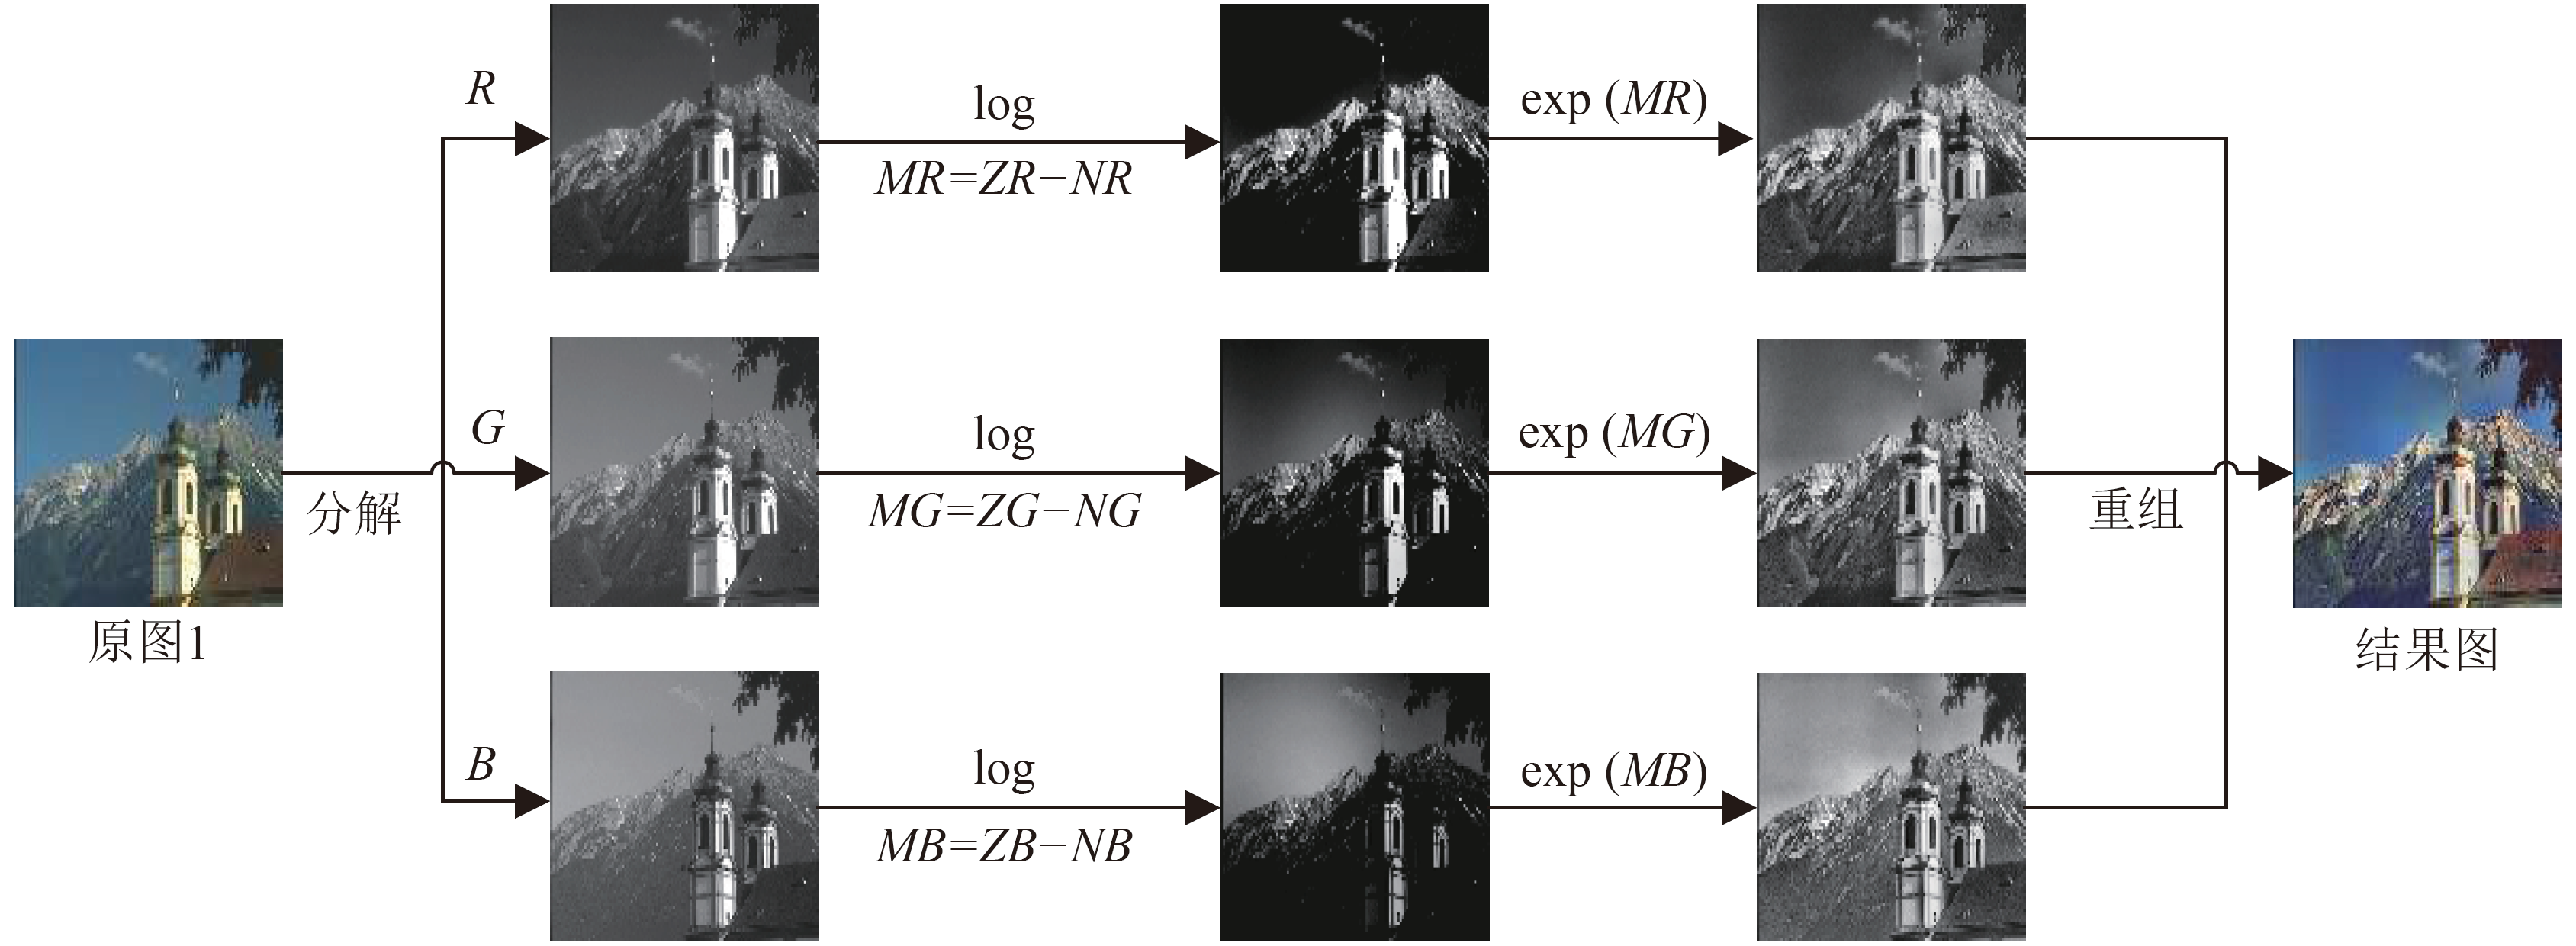
\includegraphics[width=\columnwidth]{picture/LLIE/Retinex Model/Retinex Model}
		\caption{
			\label{fig: Retinex model} 
			Retinex 算法处理过程
		}
	\end{figure}
	
	但是,传统 Retinex 算法能够很大程度改善图像质量,但在应用的过程中仍存在不可忽视的缺点。从图\ref{fig: Retinex Model}中可以看到基于传统 Retinex 算法的优势和局限性。由图\ref{fig: Retinex Model_Retinex}可见文献\cite{cooper2004analysis}算法能提高图\ref{fig: Retinex Model_input}的对比度和亮度, 整体颜色较清晰, 但天空部分的颜色并不自然, 并伴随伪影产生. 从图\ref{fig: Retinex Model_SSR}、图\ref{fig: Retinex Model_MSR}、图\ref{fig: Retinex Model_MSRCR}中明显看出, 基于中心/环绕的 Retinex 算法效果更有效. 但算法中参数选取具有局限性, 导致增强图像的对比度、色度、清晰度具有不确定性, 故增强效果并不理想。其中图\ref{fig: Retinex Model_SSR} SSR 算法能稍微改善天空的颜色, 但整体对比度有所下降, 且光晕现象较为严重; 图\ref{fig: Retinex Model_MSRCR} 中, MSRCR 算法因有颜色因子的缘故, 颜色明显要比图\ref{fig: Retinex Model_MSR} MSR 算法中图像的亮度和色度更为自然真实, 天空部分也少了许多伪影, 但改善效果仍不是最理想\cite{202013}。随着学者们对Retinex 算法的深入研究, 尤其针对传统Retinex 算法中的颜色失真和光晕现象这两大缺陷, 提出了大量的改进算法。
	
	\begin{figure}[htb] 
		\centering 
		\begin{subfigure}{0.18\textwidth}
			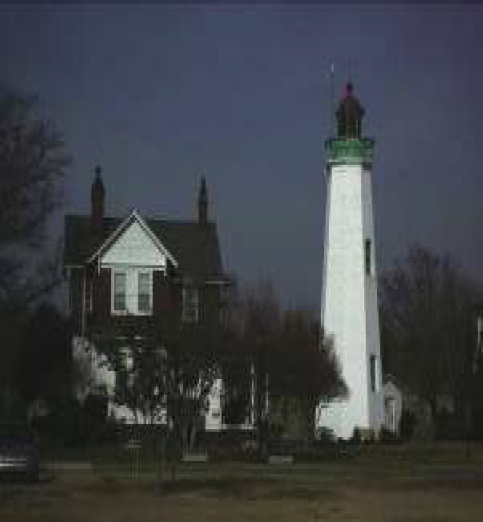
\includegraphics[width=\linewidth]{picture/LLIE/Retinex Model/input}
			\captionsetup{font=scriptsize}
			\caption{低照度图像}
			\label{fig: Retinex Model_input}
		\end{subfigure}
		\begin{subfigure}{0.18\textwidth}
			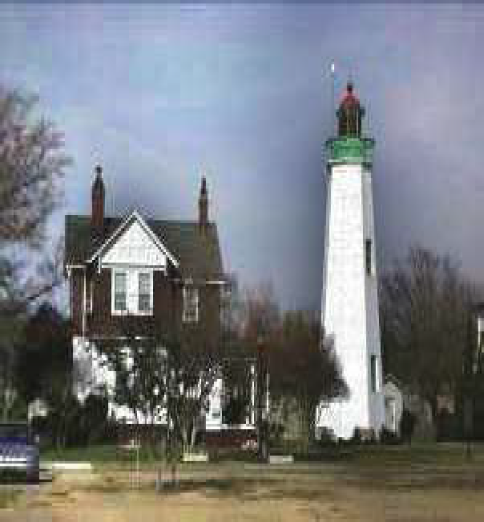
\includegraphics[width=\linewidth]{picture/LLIE/Retinex Model/Retinex}
			\captionsetup{font=scriptsize}
			\caption{Retinex\cite{cooper2004analysis}}
			\label{fig: Retinex Model_Retinex}
		\end{subfigure}
		\begin{subfigure}{0.18\textwidth}
			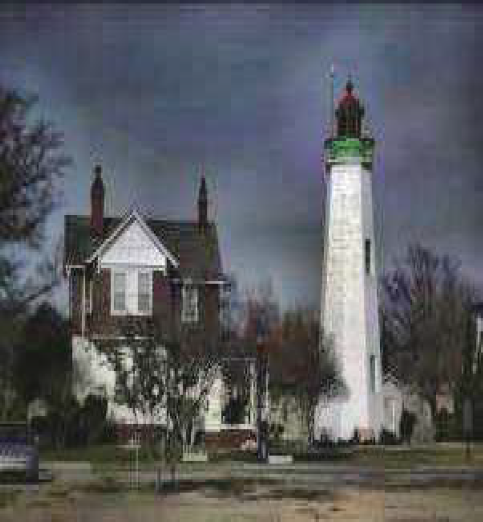
\includegraphics[width=\linewidth]{picture/LLIE/Retinex Model/SSR}
			\captionsetup{font=scriptsize}
			\caption{SSR}
			\label{fig: Retinex Model_SSR}	
		\end{subfigure}
		\begin{subfigure}{0.18\textwidth}
			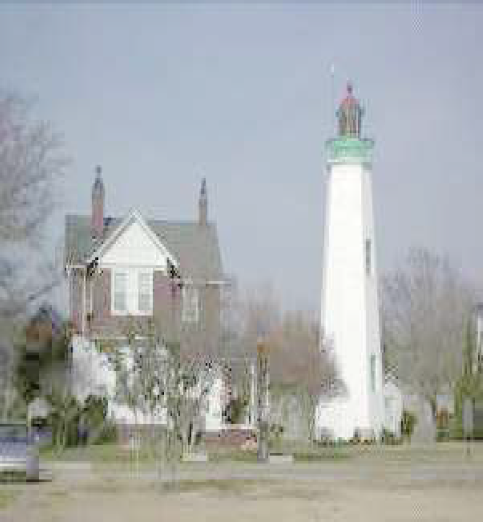
\includegraphics[width=\linewidth]{picture/LLIE/Retinex Model/MSR}
			\captionsetup{font=scriptsize}
			\caption{MSR}
			\label{fig: Retinex Model_MSR}	
		\end{subfigure}
		\begin{subfigure}{0.18\textwidth}
			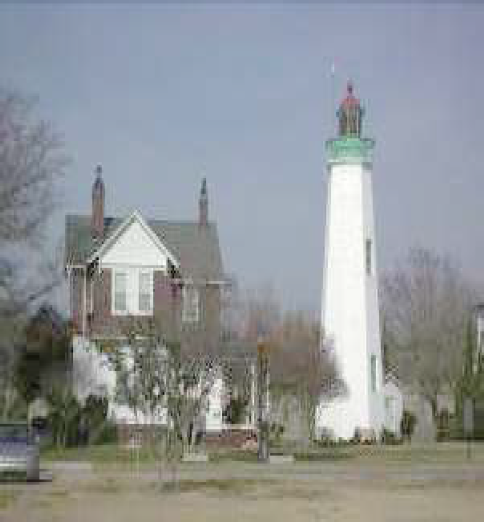
\includegraphics[width=\linewidth]{picture/LLIE/Retinex Model/MSRCR}
			\captionsetup{font=scriptsize}
			\caption{MSRCR}
			\label{fig: Retinex Model_MSRCR}	
		\end{subfigure}
		\caption{
			\label{fig: Retinex Model}
			传统 Retinex 算法实验结果。
		}
	\end{figure}
	
	\subsubsection{基于直方图的方法}
	
	基于直方图的方法主要考虑直方图均衡化\cite{stark2000adaptive},通过对直方图\footnote{直方图统计图像每个灰度级的出现频率,其横坐标表示灰度级,纵坐标表示像素值为该灰度级下像素的频率。}的分布进行约束,改善图像的亮度分布。直方图描述了图像灰度级\footnote{图像灰度(image grayscale):把白色与黑色之间按对数关系分为若干等级,称为灰度。灰度分为256阶。用灰度表示的图像称作灰度图。}的分布情况,显示了图像的灰度范围和每个灰度级的出现频率。摄影师也常利用直方图判断整幅图像的明暗程度、对比度等图像特征,以便完成相应的后期处理。
	
	\begin{figure}[htb]
		\centering 
		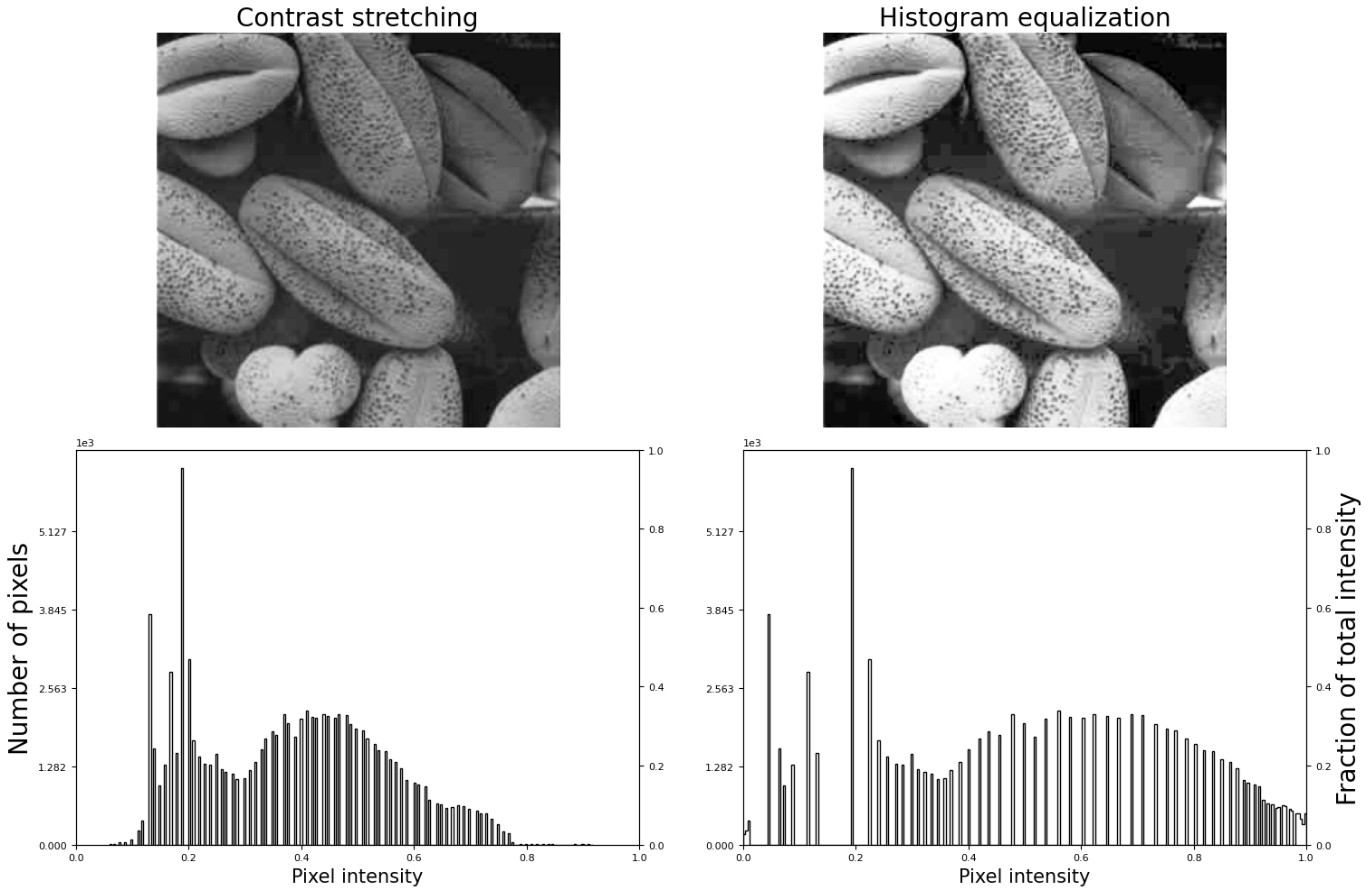
\includegraphics[width=\columnwidth]{picture/LLIE/HE/Histogram equalization}
		%\captionsetup{font=scriptsize}
		\caption{
			\label{fig: Histogram equalization} 
			直方图均衡化示意图
		}
	\end{figure}
	
	如图\ref{fig: Histogram equalization}所示,直方图均衡化重新调整图像的直方图分布,一方面增加了图像的全局对比度,另一方面使得亮度在整个图像的分布更加均匀。考虑一张包含L个灰度级的图像,其直方图可以表示为式\ref{eq: Histogram}
	\begin{equation}
		\begin{aligned}
			P(r_k) = \frac{n_k}{n}, k=0, 1, 2, \cdots, L-1
		\end{aligned}
		\label{eq: Histogram}
	\end{equation}
	其中, $r_k$ 表示第 $k$ 级灰度值,$n_k$表示图像中第 $k$ 级灰度值所对应的像素个数,$n$ 表示图像中的所有像素总数。显然,有 $\sum_{k} P(r_k)=1$。直方图均衡化是指存在一个变换函数 $s=T(r), 0 \leqslant r \leqslant 1$,能够将灰度级 $r$ 转化为灰度级 $s$。$T(r)$满足以下两个条件: 首先,$T(r)$ 在区间 $[0, 1]$ 上为单射函数且单调递增; 其次, $T(r) \in [0, 1]$ 。$T(r)$ 是单射函数保证了直方图均衡化存在反变换,而其单调递增的性质保证了变化后的图像与原图像之间存在保序性,以防变换后图像发生黑白颠倒。
	
	这样,一幅图像的灰度即视为 $[0,1]$ 上的随机变量,用 $p_r(r)$ 和 $p_s(s)$ 表示随机变量 $r$ 与 $s$的概率密度函数,那么,直方图均衡化即将 $T(r)$ 表示为式\ref{eq: HE}
	\begin{equation}
		\begin{aligned}
			s = T(r) = \int_{0}^{r} p_r(w) \mathrm{d}w
		\end{aligned}
		\label{eq: HE}
	\end{equation}
	可以证得,通过 $T(r)$ 的转化,有 $p_s(s) = 1$ ,即转换后的像素值在 $[0, 1]$ 上均匀分布。这时基于直方图变换的保序性,有 $$\int_{0}^{n} p_r(r) \mathrm{d}r = \int_{0}^{T(n)} p_s(s) \mathrm{d}s$$ 从而有: $$\frac{\mathrm{d}s}{\mathrm{d}r} = \frac{\mathrm{d}T(r)}{\mathrm{d}r} = p_r(r)$$ 代入上式,可得: $$p_s(s) = 1$$ 
	
	直方图均衡化的方法非常快速有效,并且是一个可逆操作,但缺点在于其不加选择地处理数据,可能增加背景噪声的对比度,同时降低有用的图像内容的对比度,导致视觉效果欠佳。此外,该方法也无法适用于复杂多变的低光照场景。
	
	\subsubsection{基于图像反相的方法}
	
	\begin{figure}[htbp]
		\centering 
		\begin{subfigure}{0.18\textwidth}
			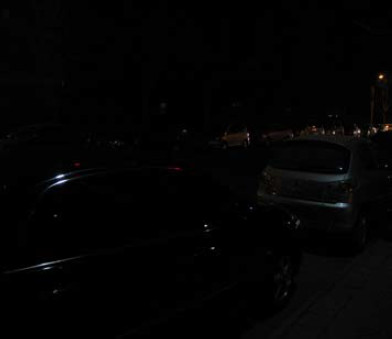
\includegraphics[width=\linewidth]{picture/LLIE/Inverse/LL input}
			\captionsetup{font=scriptsize}
			\label{fig: LL input}
		\end{subfigure}
		\begin{subfigure}{0.18\textwidth}
			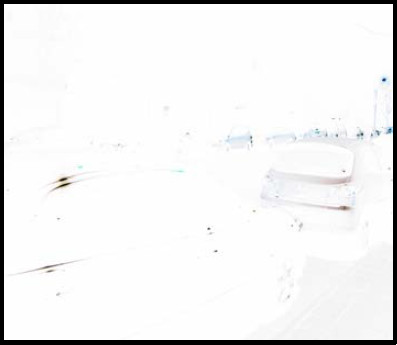
\includegraphics[width=\linewidth]{picture/LLIE/Inverse/Inversed}
			\captionsetup{font=scriptsize}
			\label{fig: Inversed}
		\end{subfigure}
		\begin{subfigure}{0.18\textwidth}
			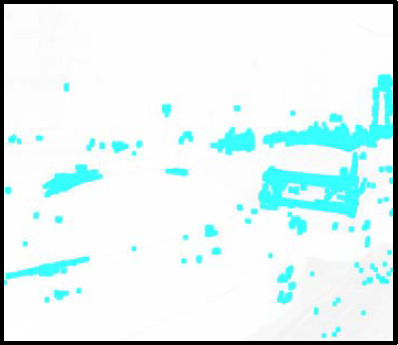
\includegraphics[width=\linewidth]{picture/LLIE/Inverse/marked image}
			\captionsetup{font=scriptsize}
			\label{fig: marked image}	
		\end{subfigure}
		\begin{subfigure}{0.18\textwidth}
			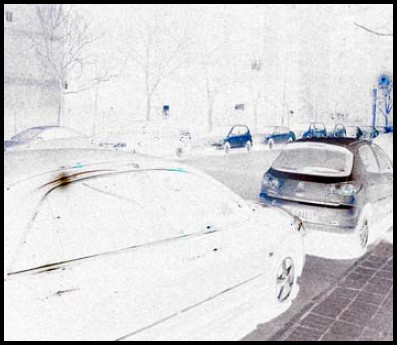
\includegraphics[width=\linewidth]{picture/LLIE/Inverse/de-haze}
			\captionsetup{font=scriptsize}
			\label{fig: de-haze}
		\end{subfigure}
		\begin{subfigure}{0.18\textwidth}
			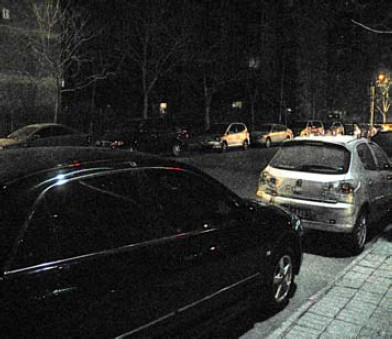
\includegraphics[width=\linewidth]{picture/LLIE/Inverse/Final output}
			\captionsetup{font=scriptsize}
			\label{fig: Final output}
		\end{subfigure}
%		\captionsetup{font=scriptsize}
		\caption{
			\label{fig: Image Inverse}
			(a) 低照度图片输入 I. (b) 从输入I获得的反向图片 R.(c) 标记图像:在至少一种颜色(RGB)通道中具有低强度的像素为绿色。 (d) 去雾: 使用公式获得输出 J. (e) 最终得输出结果 E.
		}
	\end{figure}
	
	基于图像反相的方法\cite{dong2010fast}利用低光照图像的反相\footnote{图像反相 (Image reverse phase) 就是图像的颜色色相反转。以前照相机的底片就是打印后的照片的反相。比如黑变白,蓝变黄、红变绿。对灰度级范围为 $[0 , L-1]$ 的一幅图像进行反转的操作为:$s = L - 1 - r$ 其中$r$和$s$分别代表处理前后的像素值。使用这种方式反转一幅图像的灰度级,可得到等效的照片底片。这种类型的处理特别适用于增强嵌入在一幅图像的暗区域中的白色和灰色细节,特别是当黑色面积在尺寸上占主导地位时}与有雾图像的相似性,通过对低光照图像反相进行去雾后再次进行反相,得到最终的低光照增强效果。在图像反相中,对于动态范围为 $[ 0, 255]$ 的图像,其反相图像 $\mathbf{R}$ 为式\ref{eq: Image Reverse} 
	
	\begin{equation}
		\begin{aligned}
			\mathbf{R}^c (x) = 255 - \mathbf{I}^c(x)
		\end{aligned}
		\label{eq: Image Reverse}
	\end{equation}
	
	其中,$c$ 为 \textbf{RGB} 颜色通道。大多数有雾图像符合暗通道先验,其特点是对于背景及天空等区域,\textbf{RGB} 3个通道的像素值都很高,而其他区域至少有一个通道的像素值较低,作者发现低光照图像的反相也具有同样特点。如图\ref{fig: Image Inverse}所示。
	
	基于图像反相的方法虽然运算速度很快,但需要基于低光照图像反相与有雾图像相似这一前提,而改前提始终是统计意义上的,无法得出二者之间更本质的联系,因而限制了这一方法的继续发展。由于没有考虑低光照图像的结构信息,因此该类方法还常常导致增强结构出现明显的黑边。
	
	\subsection{基于深度学习的低照度图像增强方法}
	
	从 2017 年 LLNet\cite{lore2017llnet}的出现,基于深度学习的低照度图像增强方法受到广泛关注,截至 2023 年已经出现了上百种基于深度学习的低照度图像增强方法,这充分反映了基于深度学习的方法具有更好的准确性、鲁棒性和更快的速度。
	
	基于深度学习的低照度图像增强算法,根据其学习和训练方式又分为四类,分别为有监督学习、无监督学习、半监督学习和零采样(Zero-shot)学习方法\cite{tang2023low}。
	
	\subsubsection{有监督学习}
	
	有监督学习最重要的特定是需要标记的数据集,监督学习是从标记的训练数据中学习模型,然后使用模型来训练一些新数据的标签。同时,预测标签与给点标签越相似,监督学习算法越好。基于监督学习的低照度图像增强方法大致可分为端到端 (End-to-end) 方法和 Retinex 理论方法。
	
	\paragraph{端到端 (End-to-end) 方法}
	
	\begin{figure}[htb] 
		\centering
		\begin{subfigure}{0.45\textwidth}
			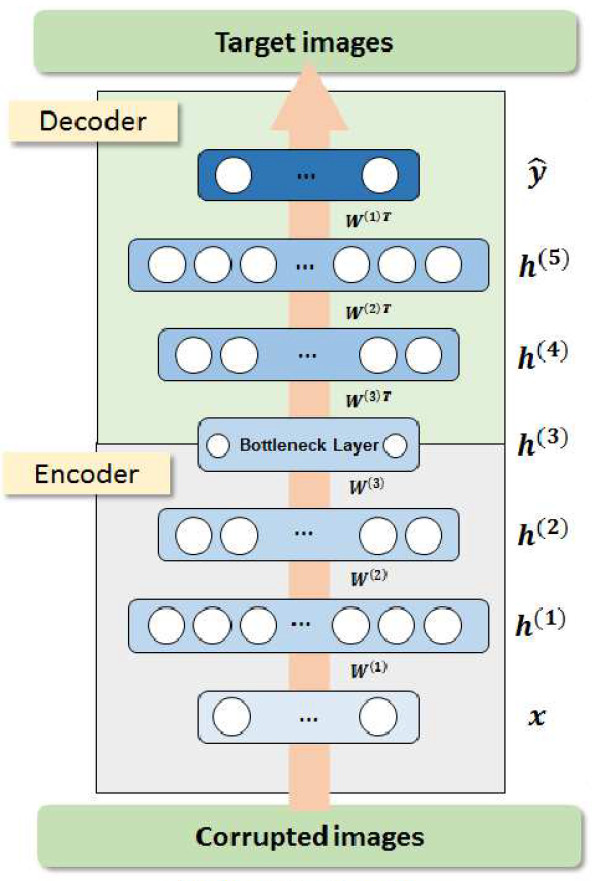
\includegraphics[width=\linewidth]{picture/LLIE/LLNet/Module Structure}
			\captionsetup{font=scriptsize}
			\caption{Module Structure}
			\label{fig: Module Structure}
		\end{subfigure}
		\begin{subfigure}{0.18\textwidth}
			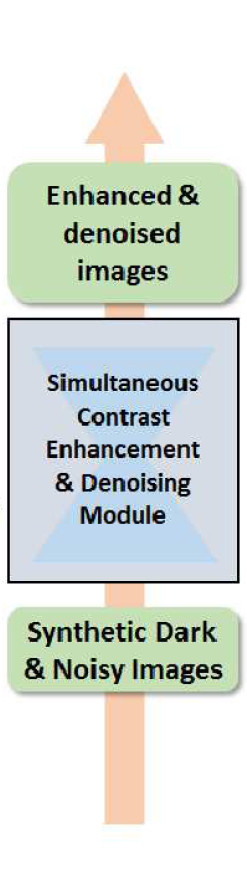
\includegraphics[width=\linewidth]{picture/LLIE/LLNet/LLNet}
			\captionsetup{font=scriptsize}
			\caption{LLNet}
			\label{fig: LLNet}
		\end{subfigure}
		\begin{subfigure}{0.175\textwidth}
			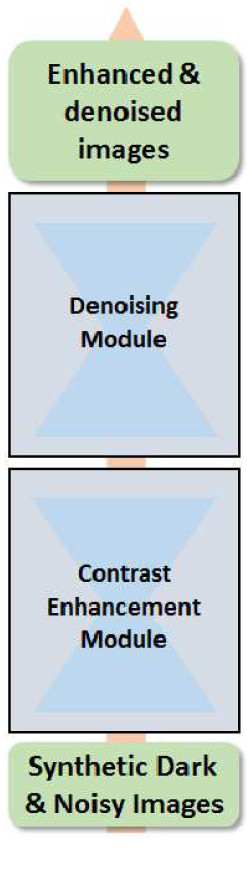
\includegraphics[width=\linewidth]{picture/LLIE/LLNet/S-LLNet}
			\captionsetup{font=scriptsize}
			\caption{S-LLNet}
			\label{fig: S-LLNet}	
		\end{subfigure}
		\caption{
			\label{fig: LLNet Architecture}
			LLNet结构示意图
		}
	\end{figure}
	
	\textbf{LLNet}\cite{lore2017llnet}是早期提出的一种基于深度学习的方法,它利用一种特殊的堆叠稀疏去噪自编码器从低光照图像中提取特征,并进行自适应增强与去噪。接着,Lv等人\cite{lv2018mbllen}介绍了 \textbf{MBLLEN},这是一个包含特征提取模块(FEM)、增强模块(EM)和融合模块(FM)的多分支图像增强网络。MBLLEN通过多层次的特征提取和多子网络的增强处理,最终通过融合模块产生增强后的图像,有效地减少低照度区域的噪声和伪影。
	
	\begin{figure}[htb]
		\centering 
		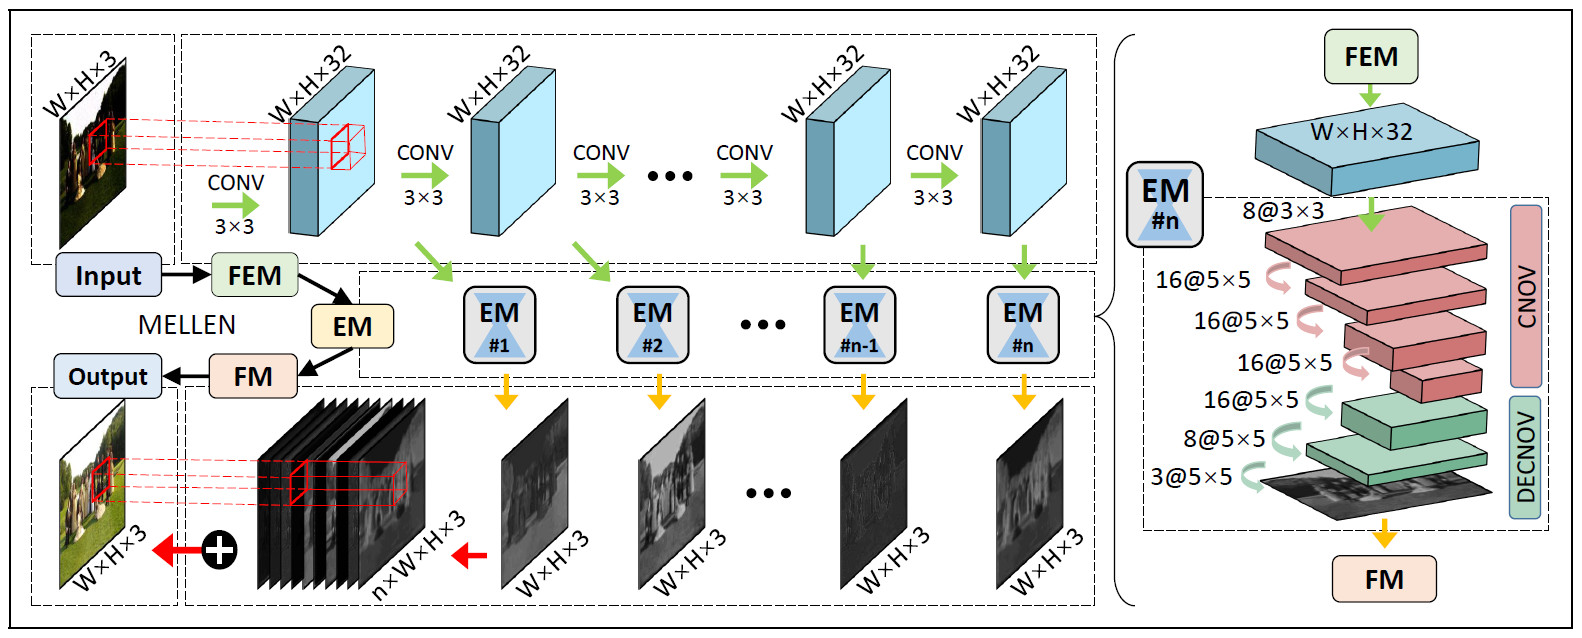
\includegraphics[width=\columnwidth]{picture/LLIE/MBLLEN/MBLLEN Architecture}
		%\captionsetup{font=scriptsize}
		\caption{
			\label{fig: MBLLEN Architecture} 
			MBLLEN 结构图。
		}
	\end{figure}
	
	此外,Wang 等人\cite{wang2018gladnet}提出的 \textbf{GLADNet} 网络使用编码器-解码器架构处理输入图像,生成全局照度估计,并在此基础上进行图像重构。该网络的有效性通过Google Cloud Vision API2上的目标识别测试得到了验证。\textbf{TBEFN}\cite{lu2020tbefn}是一种多曝光融合网络,通过两个子网络生成增强图像,进而通过平均融合法降低噪声,并对效果进行细化。\textbf{PRIEN}\cite{li2021low}是一种使用递归层和残差块的递归单元的渐进式增强网络,它直接将低照度图像输入到双注意模型中提取特征,并通过递归处理减少参数数量,尽管网络结构简单,但增强效果显著。最后,\textbf{C-LIENet}\cite{ravirathinam2021c}包含一个由卷积层构成的编码器-解码器结构,并通过其独特的多上下文特征提取模块层级提取特征,该方法采用了一种三部分的损失函数,有效地处理局部特征、结构相似性和细节性。另外,Lim等人\cite{lim2020dslr}提出的深度拉普拉斯复原器(\textbf{DSLR})能够调整输入图像的全局亮度和局部细节,并通过多尺度拉普拉斯残差块在特征空间中增强连接,提高了训练的效率。
	
	\paragraph{Retinex 理论方法}
	
	\begin{figure}[htb]
		\centering 
		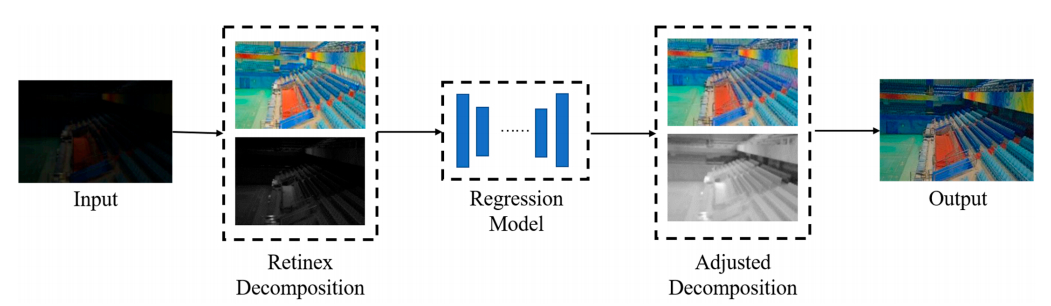
\includegraphics[width=0.7\columnwidth]{picture/LLIE/RetinexNet/RetinexNet}
		%\captionsetup{font=scriptsize}
		\caption{
			\label{fig: RetinexNet} 
			RetinexNet算法结构图。主要由三个部分组成,分解(Decomposition),调节(Adjustment)和重构(Reconstruction)。
		}
	\end{figure}
	
	相较于传统的端到端网络学习方法,融合深度学习与 Retinex 理论的策略在某些情况下展现出了更优越的图像增强性能。Wei等人\cite{wei2018deep}率先结合数据驱动方法与 Retinex 理论,开发出了一种深度学习框架 \textbf{RetinexNet}。这个框架通过分解网络将图像拆分为反射率图和结构感知的照明图,随后利用增强网络对大范围的照明区域进行优化。图像的最终效果通过局部裁剪和 BM3D 去噪技术得到提升。Liang等人\cite{shen2017msr}对MSR(多尺度Retinex)理论进行了深入的探究,并提出了 \textbf{MSR-net},它包含了多尺度对数变换、卷积差分和颜色恢复等三个模块。这个网络通过学习由 Photoshop 调整的合成低照度图像对,实现了从低照度到真实图像的直接端到端映射。\textbf{KinD}\cite{zhang2019kindling}则基于 Retinex 理论构建了一个分为照明调节和退化去除两个分支的深度网络。该网络包括层分解、反射率恢复和照度调整三个模块,并通过多尺度照度增强模块来减少增强图像的噪声和失真。
	
	\paragraph{基于 Transformer 的方法}
	
	当前,以 Vision Transformer(ViT) 为核心的监督学习任务受到广泛关注。在这一领域中,Cui等人\cite{cui2022illumination}开发了一种名为照明自适应变压器 (Illumination-Adaptive Transformer, \textbf{IAT}) 的网络。这个网络是全监督训练模式下的超轻量级架构。它借鉴了目标检测网络 \textbf{DETR} (Detection Transformer)的设计理念\cite{carion2020end},实现了一个端到端的变压器结构,有效地解决了低照度环境下的视觉效果问题。IAT网络的主要优点在于其出色的性能和快速的处理速度。另一方面,Wang等人\cite{wang2023ultra}提出了一种新型的低照度变压器网络,名为\textbf{LLFormer}。LLFormer的关键特性是其基于轴的多头自注意力和跨层注意力融合块,这大大减少了计算的复杂度。此外,Wang等人还创建了一个4K和8K超高清图像(UHD-LOL)的基准数据集,用以评估LLFormer的性能。这代表了首次尝试解决超高清低照度图像增强(UHD-LLIE)的任务。
	
	\subsubsection{无监督学习}
	
	尽管有监督学习方法在图像增强中取得了一定的成效,但它面临着两大主要限制。首先,可用于训练的成对图像数据集是有限的。其次,在这样的成对数据集上训练的模型容易出现过拟合的问题。为了克服这些挑战,研究者们转向了无监督学习方法。无监督学习的主要特点是在没有标签数据的情况下进行学习。Jiang等人\cite{jiang2021enlightengan}开创性地提出了一种名为 \textbf{EnlightenGAN} 的无监督学习方法。这是首个在该领域成功应用非配对训练的例子。EnlightenGAN的主要创新在于两个方面:一是其全局-局部判别器结构,用于处理输入图像中的空间光照变化;二是结合自特征保留损失和自正则化注意力机制,确保增强后图像的内容特征保持不变。此外,Fu等人\cite{fu2022gan}设计了一种名为 \textbf{LE-GAN} 的低照度增强网络,使用不变身份损失和注意力模块来提升图像特征提取,同时实现降噪和细节增强。该网络通过不变身份损失解决过度曝光的问题。他们还构建并公开了一个较大的非配对低照度/正常照度图像数据集PNLI。
	
	\begin{figure}[htb]
		\centering 
		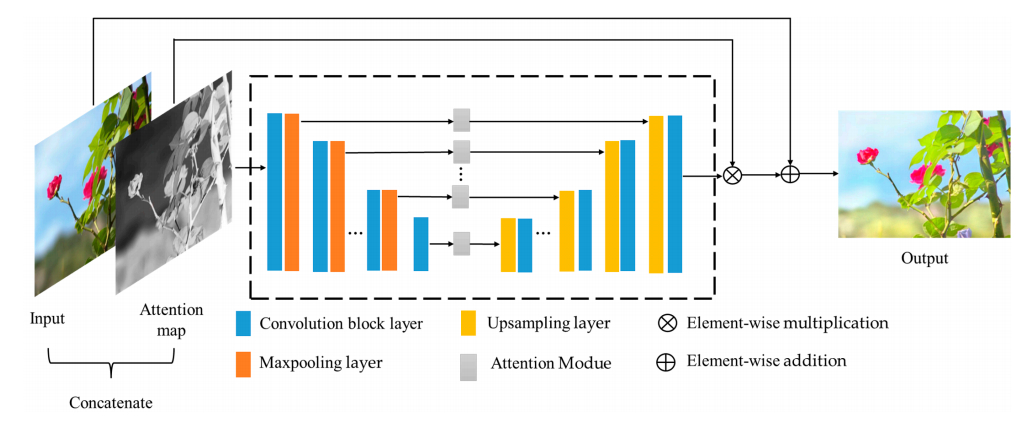
\includegraphics[width=0.7\columnwidth]{picture/LLIE/EnlightenGAN/EnlightenGAN}
		%\captionsetup{font=scriptsize}
		\caption{
			\label{fig: EnlightenGAN} 
			EnlightenGAN 结构图
		}
	\end{figure}
	
	Ni等人\cite{ni2020towards}提出了 \textbf{UE-GAN},一种基于单个深度GAN并结合注意力机制的无监督增强方法。UE-GAN 通过引入保真度损失和质量损失来处理无监督图像增强,确保增强后的图像在内容上与输入图像保持一致。Zhang等人\cite{zhang2021unsupervised}则提出了一种基于直方图均衡化的无监督低照度图像增强方法 \textbf{HEP}。该方法采用噪声分离模块(NDM),对非配对图像对的反射率图中的噪声和内容进行分离,并通过直方图均衡化和噪声分离模块有效增强图像的纹理信息和亮度细节,同时抑制图像暗黄色区域的噪声。
	
	\subsubsection{半监督学习}
	
	近年来,半监督学习作为一种新兴的学习方法,结合了监督学习的精确性和非监督学习的广泛适用性。这种学习方法既利用了有标签的数据,也依赖于无标签的数据。其显著特点是能够在有限的标记样本和大量未标记样本的情况下训练有效的分类器,从而解决在标记样本稀缺、未标记样本丰富的情境下的学习问题。
	
	\begin{figure}[htb]
		\centering 
		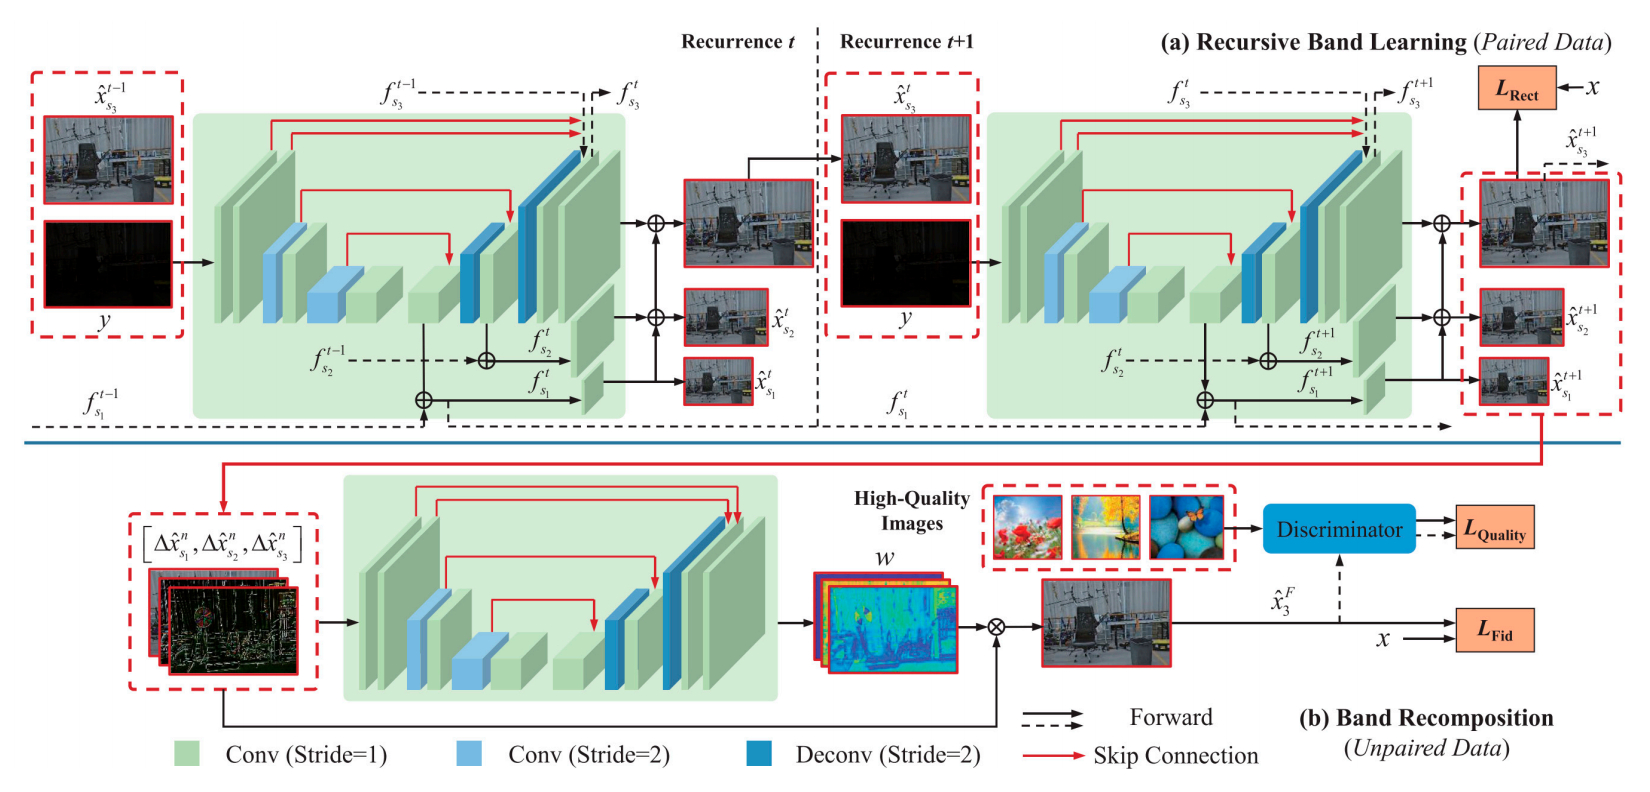
\includegraphics[width=0.7\columnwidth]{picture/LLIE/DRBN/DRBN}
		%\captionsetup{font=scriptsize}
		\caption{
			\label{fig: DRBN} 
			DRBN 结构图
		}
	\end{figure}
	
	在这一领域中,Yang等人\cite{qiao2021deep}提出了一种名为 \textbf{DRBN} 的半监督低照度图像增强方法,该方法基于频带表示。DRBN是一种深度递归频带网络,它通过对低光照/标准光照图像对的频带表示进行线性恢复,然后对这些频带进行重新定位,以改善频带表示。这种方法不仅有效地去除了图像噪声,还能优化图像细节。另一方面,Robert等人开发了一种名为 \textbf{HybirdNet} 的半监督学习网络\cite{robert2018hybridnet}。该网络分为两个分支:第一个分支接收监督信号并专注于提取不变的成分,而第二个分支完全无监督,其目的是重建第一个分支丢弃的模型信息,作为输入数据的补充。
	
	\subsubsection{Zero-Shot 学习}
	
	Zero-shot 学习的一个显著优点是它无需依赖预先训练的数据集。这种方法允许直接将待处理的低光照图像作为输入,而无需经过预先的训练阶段。在这一方法论下,Zhu等人\cite{zhu2020zero}提出了一种创新的三分支全卷积神经网络,名为\textbf{RRDNet}。该网络将输入图像拆分为三个组成部分:光照、反射和噪声。通过特殊设计的迭代损失函数,网络能够对噪声进行精确估计并有效恢复光照部分,实现清晰的噪声预测,进而成功去除图像中的噪声。RRDNet还引入了一种新型的损失算法,该算法依据图像的亮度分布来估计暗区的噪声,避免了暗区噪声的过度放大。受到超分辨率模型的启发,Zhang等人\cite{zhang2019zero}开发了一种专门用于实时测试的CNN网络\textbf{ExCNet}。在实际应用中,ExCNet能够估计出最适合当前背光图像的参数曲线,这使得网络非常适合在复杂拍摄环境和恶劣的背光条件下进行图像增强。ExCNet的一个独特优势是其能够利用前一帧的参数作为参考,从而在视频增强过程中避免产生伪影。
	
	\begin{figure}[htb]
		\centering 
		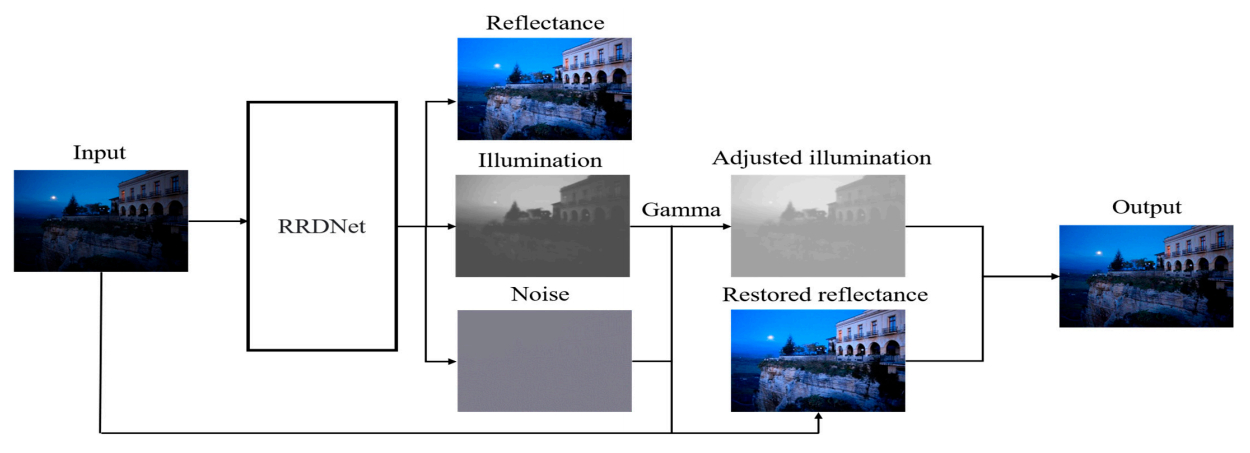
\includegraphics[width=0.7\columnwidth]{picture/LLIE/RRDNet/RRDNet}
		\caption{
			\label{fig: RRDNet} 
			RRDNet 结构图
		}
	\end{figure}
	
	\subsection{数据集}
	
	LOL\cite{wei2018deep}和LE-LOL-L\cite{liu2021benchmarking}数据集的测试图像的客观评价指标值比 SCIE\cite{cai2018learning} 和 LIME\cite{guo2016lime} 数据集更适合人类视觉效果。用成对数据集训练的算法将得到更明显的增强效果。从数据中可以看出,基于监督学习的方法比其他方法更能取得更好的效果。
	
	然而,无监督学习、Zero-Shot学习和半监督学习是当前的发展趋势,主要是因为在低光照环境下很难获得成对的图像。与其他方法相比,基于完全监督学习的方法泛化能力较低,适用性较差。此外,无监督学习方法可以通过设计适当的损失函数和网络结构,引入更多反映环境特征的先验知识。
	
	\subsection{评价指标}
	
	\subsubsection{客观评价指标}
	
	图像的客观评价指标很多,不同角度的评价标准也不尽相同。每种评价标准都有其相应的优缺点。到目前为止,还没有明确设计用于微光图像增强的评估指标。现有的图像质量评价方法可分为完全参考评价指标和无参考评价指标。
	
	\textbf{完全参考评价指标}需要有一个完整的参考图像(即原始图像或专家标注的高质量图像)作为参照。通过将待评价的图像与参考图像进行比较,计算它们之间的差异来评估图像的质量。常见的完全参考评价指标包括:均方误差(Mean Square Error,MSE)、峰值信噪比(Peak Signal-to-Noise Ratio,PSNR)、结构相似性指数(Structural Similarity Index,SSIM)
	
	\begin{table}[!htbp]
		\centering
		\small
		%\resizebox{\textwidth}{!}{ %按照宽度调整调整表格大小
			\begin{tabular}{cc}
				
				\toprule
				
				\textbf{Abbreviation} & \textbf{Full-/Non-Reference} \\
				
				\hline
				
				MSE (Mean Square Error)\cite{singh2016contrast,dong2010fast} & Full-Reference \\
				MAE (Mean Absolute Error)\cite{chai2014root} & Full-Reference \\
				SNR (Signal to Noise Ratio)\cite{kellman2005image} & Full-Reference \\
				PSNR (Peak-Signal to Noise Ratio)\cite{yu2017low} & Full-Reference \\
				LPIPS (Learned Perceptual Image Patch Similarity)\cite{zhang2018unreasonable} & Full-Reference \\
				IFC (Information Fidelity Criterion)\cite{sheikh2005information} & Full-Reference \\
				VIF (Visual Information Fidelity)\cite{russakovsky2015imagenet} & Full-Reference \\
				SSIM (Structural Similarity Index)\cite{ignatov2018wespe} & Full-Reference \\
				IE (Information Entropy)\cite{zhu2015low} & Non-Reference \\
				NIQE (Natural Image Quality Evaluator)\cite{mittal2012making} & Non-Reference \\
				LOE (Lightness Order Error)\cite{fu2016weighted} & Full-Reference \\
				PI (Perceptual Index)\cite{ma2017learning} & Non-Reference \\
				MUSIQ (Multi-scale Image Quality Transformer)\cite{ke2021musiq} & Non-Reference \\
				NIMA (Neural Image Assessment)\cite{talebi2018nima} & Non-Reference \\
				SPAQ (Smartphone Photography Attribute and Quality)\cite{fang2020perceptual} & Non-Reference \\
				
				\bottomrule
				
			\end{tabular}
			%}
		%	\captionsetup{font=scriptsize}
		\caption{\label{tab: quality evaluation index}
			图像的客观质量评价指标
		} %表格的标题
	\end{table}
	
	\textbf{无参考评价指标}不需要参考图像,仅通过待评价图像自身的特征来评估图像质量。这些指标主要基于图像的统计特性、信息熵等,无需外部参考信息。常见的无参考评价指标包括:
	
	\begin{itemize}
		\item [(1)] 图像清晰度评估:通过图像的锐度、对比度等特征来评估图像的清晰度和质量。
		
		\item [(2)] 图像亮度评估:基于图像的亮度直方图、灰度均值等特征,评估图像的亮度质量。
		
		\item [(3)] 图像块失真评估:通过比较图像中局部块之间的差异,来评估图像的块状失真程度。
	\end{itemize}
	
	表\ref{tab: quality evaluation index} 列出了最新的几个经典关键的质量评价指标。
	
	\paragraph{峰值信噪比 (Peak-Signal to Noise Ratio, PSNR)} 峰值信噪比(PSNR)是应用最广泛的指标之一。单位为dB。它用于测量两个图像之间的差异。如压缩图像与原始图像、压缩图像质量评估、恢复图像与实际图像、恢复算法性能评估等。PSNR值越高,失真越小。PSNR的公式为式\ref{eq: PSNR}
	\begin{equation}
		\begin{aligned}
			\text{PSNR} = 10 \times \log \frac{\text{{MaxValue}}^2}{\text{MSE}}
		\end{aligned}
		\label{eq: PSNR}
	\end{equation}
	
	其中MSE是两个图像的均方误差;MaxValue是图像像素的最大值。
	
	\paragraph{结构相似性 (Structural Similarity, SSIM)} 结构相似性(SSIM)是参考图像质量评价中应用最广泛的标准。SSIM用于突出值范围为0–1的两幅图像之间的亮度、对比度和结构相似性;越接近1,两个图像就越相似。假设x和y是两个输入图像,SSIM的公式为式\ref{eq: SSIM_eq}
	\begin{equation}
		\begin{aligned}
			\text{SSIM} = {\left[ l(x,y) \right]}^{\alpha} {\left[C(x,y)\right]}^\beta {\left[S(x,y)\right]}^\gamma
		\end{aligned}
		\label{eq: SSIM_eq}
	\end{equation}
	
	其中,$l(x,y)$是亮度比较,$C(x,y)$是对比度比较,$S(x,y)$是结构比较。$\alpha, \beta, \gamma$大于$0$,用于调节三部分比重。$l(x, y)$、$C(x, y)$和$S(x, y)$分别为式\ref{eq: l(x,y)}, 式\ref{eq: C(x,y)}, 式\ref{eq: (x, y)}
	
	\begin{equation}
		\begin{aligned}
			l(x,y)=\frac{2\mu_x \mu_y + c_1}{\mu x^2 + \mu y^2 + c_1}
		\end{aligned}
		\label{eq: l(x,y)}
	\end{equation}
	
	\begin{equation}
		\begin{aligned}
			C(x,y) = \frac{2\sigma_{xy}+c_2}{\sigma_x^2 + \sigma_ y^2 + c^2}
		\end{aligned}
		\label{eq: C(x,y)}
	\end{equation}
	
	\begin{equation}
		\begin{aligned}
			(x, y) = \frac{\sigma_{xy} + c_3}{\sigma_{x}\sigma_{y} + c_3}
		\end{aligned}
		\label{eq: (x, y)}
	\end{equation}
	
	其中$\mu_x$和$\mu_y$表示两幅图像的平均值,$\sigma_x$和$sigma_y$分别表示两幅图的标准差。$\sigma_xy$表示两个图像的协方差。$c_1$、$c_2$和$c_3$是常数,以避免分母为0。
	
	\paragraph{均方误差 (Mean Square Error, MSE)}
	
	均方误差(MSE)也是衡量图像质量最常用的指标之一。它是指估计值与真实值之间的平方差的期望值。在图像处理算法中,它是被处理后的图像像素值与原始像素值之间的平方差的平均值。MSE表达式如式\ref{eq: MSE}
	\begin{equation}
		\begin{aligned}
			\text{MSE} = \frac{1}{M \times N} \sum_{i=1}^{M} \sum_{N}^{j=1}{\left[ g(x,y) - \hat{g}(x,y) \right]}^2
		\end{aligned}
		\label{eq: MSE}
	\end{equation}
	
	其中,$M$是图像的高度,$N$是图像的宽度。$g(x,y)$和$\hat{g}(x,y)$分别表示原始图像和增强图像。MSE的值越小,图像质量越好。
	
	
	\paragraph{信息熵 (Information Entropy, IE)}
	
	信息熵(IE)反映了图像所携带的信息量。信息熵越大,图像信息越丰富,质量越好。IE用于比较不同图像中信息内容的差异。例如,在同一区域拍摄的图像也会由于额外的拍摄时间而具有不同的信息内容。IE表达式式\ref{eq: IE}
	\begin{equation}
		\begin{aligned}
			\text{H} = -\sum_{i=0}^{M} p(k)\log_{2}p(k)
		\end{aligned}
		\label{eq: IE}
	\end{equation}
	
	其中$p(k)$是灰度级$k$的概率密度,$M$是最大灰度级
	
	\paragraph{标准偏差 (Standard Deviation, STD)}
	
	标准差(STD),也称为标准差,表示每个数据项与平均值的平均距离。STD也是方差的平方根。STD可以反映数据集的分散程度。与图像相比,STD反映了插图与平均值之间的分散程度,是特定范围内图像对比度的衡量标准。标准偏差越大,图像中包含的信息越多,视觉效果越好。STD的表达式式\ref{eq: STD}
	\begin{equation}
		\begin{aligned}
			\text{STD} = \sqrt{\frac{\sum_{i=1}^{M} \sum_{j=1}^{N} f(i,j)\left( f(i,j)-\delta \right)^{2}}{M \times N}}
		\end{aligned}
		\label{eq: STD}
	\end{equation}
	
	其中$M$是图像的高度,$N$是图像的宽度,$f(i, j)$表示图像的$(i, j)$处的像素的灰度值。$\delta$表示图像的平均灰度值,其表达式为式\ref{eq: delta}
	\begin{equation}
		\begin{aligned}
			\delta = \frac{1}{M \times N} \sum_{i=1}^{M} \sum_{j=1}^{N} f(i,j)
		\end{aligned}
		\label{eq: delta}
	\end{equation}
	
	\paragraph{亮度顺序误差 (Lightness Order Error, LOE)}
	
	亮度顺序误差(LOE)是图像亮度的顺序差异,并且通过评估图像在邻域中的亮度的顺序变化过程来评估图像的照度变化。LOE反映了图像的自然保持能力。较小的值表示图像具有更好的亮度顺序并且看起来更自然。表达式为式\ref{eq: LOE}
	\begin{equation}
		\begin{aligned}
			\text{RD}(i,j) = \sum_{x}^{M} \sum_{y}^{N} U\left( L(i,j), L(x,y) \right) \oplus U\left( L_{e}(i,j), L(x,y) \right) 
		\end{aligned}
		\label{eq: LOE}
	\end{equation}
	
	式中,$M$是图像的高度,$N$是图像的宽度,而$\oplus$是XOR算子,$L(i, j)$和$L_{e}(x, y)$分别表示三个颜色通道中的最大值。LOE的值越小,图像保持的亮度顺序越好。
	
	\subsubsection{主观评价指标}
	
	\paragraph{差分平均意见分数 (Differential Mean Opinion Score, MOS)}
	
	差分平均意见得分(MOS)或差分平均看法得分(DMOS)。其中,MOS是应用最广泛的主观IQA方法。不同的人在原始图像和增强图像之间进行主观比较,以获得MOS分数,最后获得平均分数。MOS评分范围从1到5,评分越高表示主观增强越好。MOS评分公式为式\ref{MOS}
	\begin{equation}
		\begin{aligned}
			\text{MOS} = \frac{\sum_{n=1}^{N} R_{n}} {N}
		\end{aligned}
		\label{eq: MOS}
	\end{equation}
	
	其中$R$表示评价者对图像的满意度得分的数量,$N$表示评价者的总数。
	
	\section{研究目的}
	
	\subsubsection{现有方法的局限性}
	
	现有的方法仍有很大的改进空间,例如如何在提高亮度的同时消除产生的噪声,如何避免颜色失真现象等。一些现有的方法可以有效地解决一个问题,但往往会忽略了其他问题。不同的方法在不同的数据集上往往具有不同的优势,即在不同的评估标准下有不同的优势,如图\ref{fig: VE-LOL-L Visual}展示了不同算法在VE-LOL-L数据集下的可视化结果。
	
	\begin{figure}[htbp]
		\centering
		\begin{subfigure}{0.17\columnwidth}
			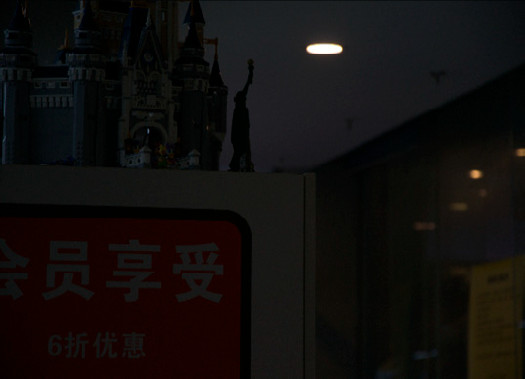
\includegraphics[width=\linewidth]{picture/LLIE/VE-LOL-L/input}
			\captionsetup{font=scriptsize}
			\caption*{input \\ \quad }
			\label{fig: input}
		\end{subfigure}
		\begin{subfigure}{0.17\columnwidth}
			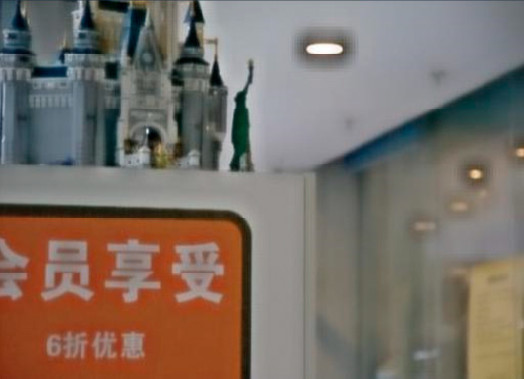
\includegraphics[width=\linewidth]{picture/LLIE/VE-LOL-L/LLNet}
			\captionsetup{font=scriptsize}
			\caption*{LLNet \\ (2017)}
			\label{fig: LLNet_VE_LOL}	
		\end{subfigure}
		\begin{subfigure}{0.17\columnwidth}
			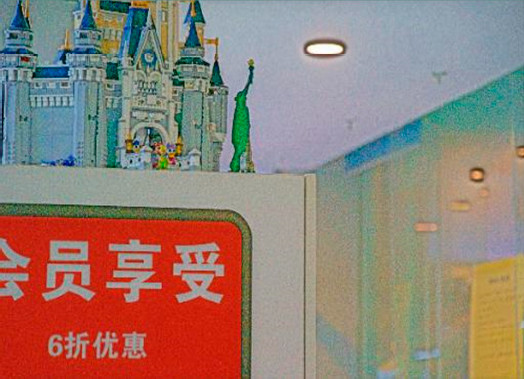
\includegraphics[width=\linewidth]{picture/LLIE/VE-LOL-L/RetinexNet}
			\captionsetup{font=scriptsize}
			\caption*{RetinexNet \\ (2018)}
			\label{fig: RetinexNet_VE_LOL}	
		\end{subfigure}
		\begin{subfigure}{0.17\columnwidth}
			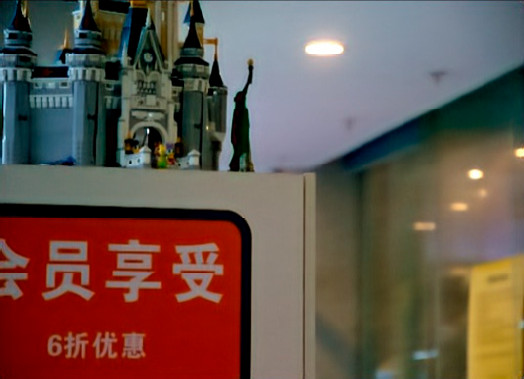
\includegraphics[width=\linewidth]{picture/LLIE/VE-LOL-L/MBLLEN}
			\captionsetup{font=scriptsize}
			\caption*{MBLLEN \\ (2018)}
			\label{fig: MBLLEN_LOL}	
		\end{subfigure}
		\begin{subfigure}{0.17\columnwidth}
			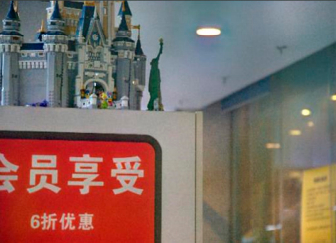
\includegraphics[width=\linewidth]{picture/LLIE/VE-LOL-L/EnlightenGAN}
			\captionsetup{font=scriptsize}
			\caption*{EnlightenGAN \\ (2019)}
			\label{fig: EnlightenGAN_VE_LOL}	
		\end{subfigure}
		\begin{subfigure}{0.17\columnwidth}
			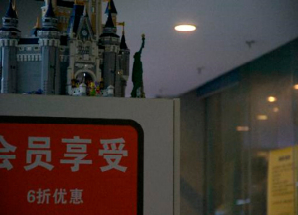
\includegraphics[width=\linewidth]{picture/LLIE/VE-LOL-L/RRDNet}
			\captionsetup{font=scriptsize}
			\caption*{RRDNet \\ (2020)}
			\label{fig: RRDNet_VE_LOL}	
		\end{subfigure}
		\begin{subfigure}{0.17\columnwidth}
			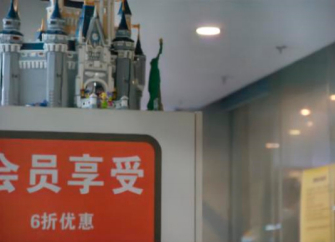
\includegraphics[width=\linewidth]{picture/LLIE/VE-LOL-L/DRBN}
			\captionsetup{font=scriptsize}
			\caption*{DRBN \\ (2020)}
			\label{fig: DRBN_VE_LOL}	
		\end{subfigure}
		\begin{subfigure}{0.17\columnwidth}
			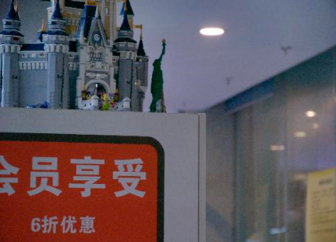
\includegraphics[width=\linewidth]{picture/LLIE/VE-LOL-L/Zero-DCE++}
			\captionsetup{font=scriptsize}
			\caption*{Zero-DCE++ \\ (2021)}
			\label{fig: Zero-DCE++}	
		\end{subfigure}
		\begin{subfigure}{0.17\columnwidth}
			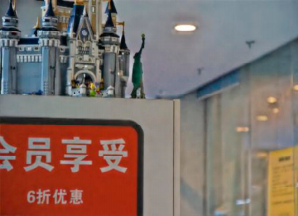
\includegraphics[width=\linewidth]{picture/LLIE/VE-LOL-L/KinD++}
			\captionsetup{font=scriptsize}
			\caption*{KinD++ \\ (2021)}
			\label{fig: KinD++}	
		\end{subfigure}
		\begin{subfigure}{0.17\columnwidth}
			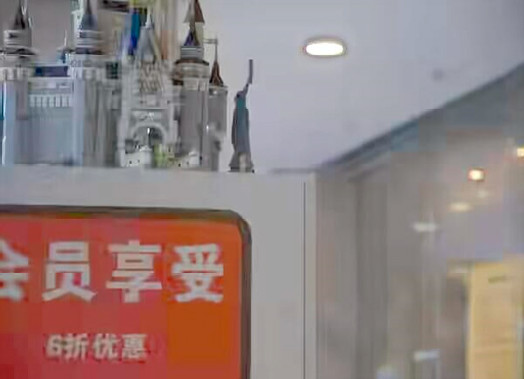
\includegraphics[width=\linewidth]{picture/LLIE/VE-LOL-L/URetinexNet}
			\captionsetup{font=scriptsize}
			\caption*{URetinexNet \\ (2022)}
			\label{fig: URetinexNet}	
		\end{subfigure}
		\caption{
			\label{fig: VE-LOL-L Visual} 
			不同算法对从 VE-LOL-L 数据集采样的低照度图像的可视化结果。 
		}
	\end{figure}
	
	近年来,基于深度学习的低光图像增强(LLIE)技术取得了显著成就,它使用神经网络来学习从弱光图像到自然光图像的映射。与传统方法相比,基于深度学习的解决方案在准确性、鲁棒性和处理速度方面表现更优,因此受到了广泛关注。特别是卷积神经网络(CNN)在多个计算机视觉任务中展现出卓越的性能。CNN通过利用注意力机制和\cite{yang2021locally, zhang2020attention}上下文信息,能够从原始图像中有效提取多尺度特征\cite{li2018multi, zamir2020learning}。在这些成果的推动下,基于CNN的低光图像增强方法得到了持续发展。例如,一种基于CNN的自适应低光图像增强框架\cite{li2020visual}显著提升了图像的对比度、颜色和细节信息。然而,现有的基于CNN的方法大多集中于图像亮度、纹理和颜色的恢复,对于局部光照不均匀、颜色信息和细节信息的丢失问题,仍存在过增强或增强不足的挑战。
	
	现有的方法可能无法在极暗或极亮的区域恢复图像边缘细节\cite{xu2023low},如图\ref{fig: SNR (CVPR 2022)}和图\ref{fig: SMG-LLIE}所示,暗区结构细节模糊。同时,当物体边缘不清晰时,像素级损失往往会模糊边缘,破坏图像细节。而加入边缘先验可以降低优化外观重构时的不适定程度。人类视觉系统对边缘高度敏感,保留结构信息对图像重建任务的性能至关重要。定义边缘可以通过学习区分黑暗区域的不同物体来指导增强过程,而不仅仅是识别低光区域。通过保留图像中的结构属性,这使得物体之间的可见性更好。
	
	\begin{figure}[htb]
		\centering
		\begin{subfigure}{0.45\columnwidth}
			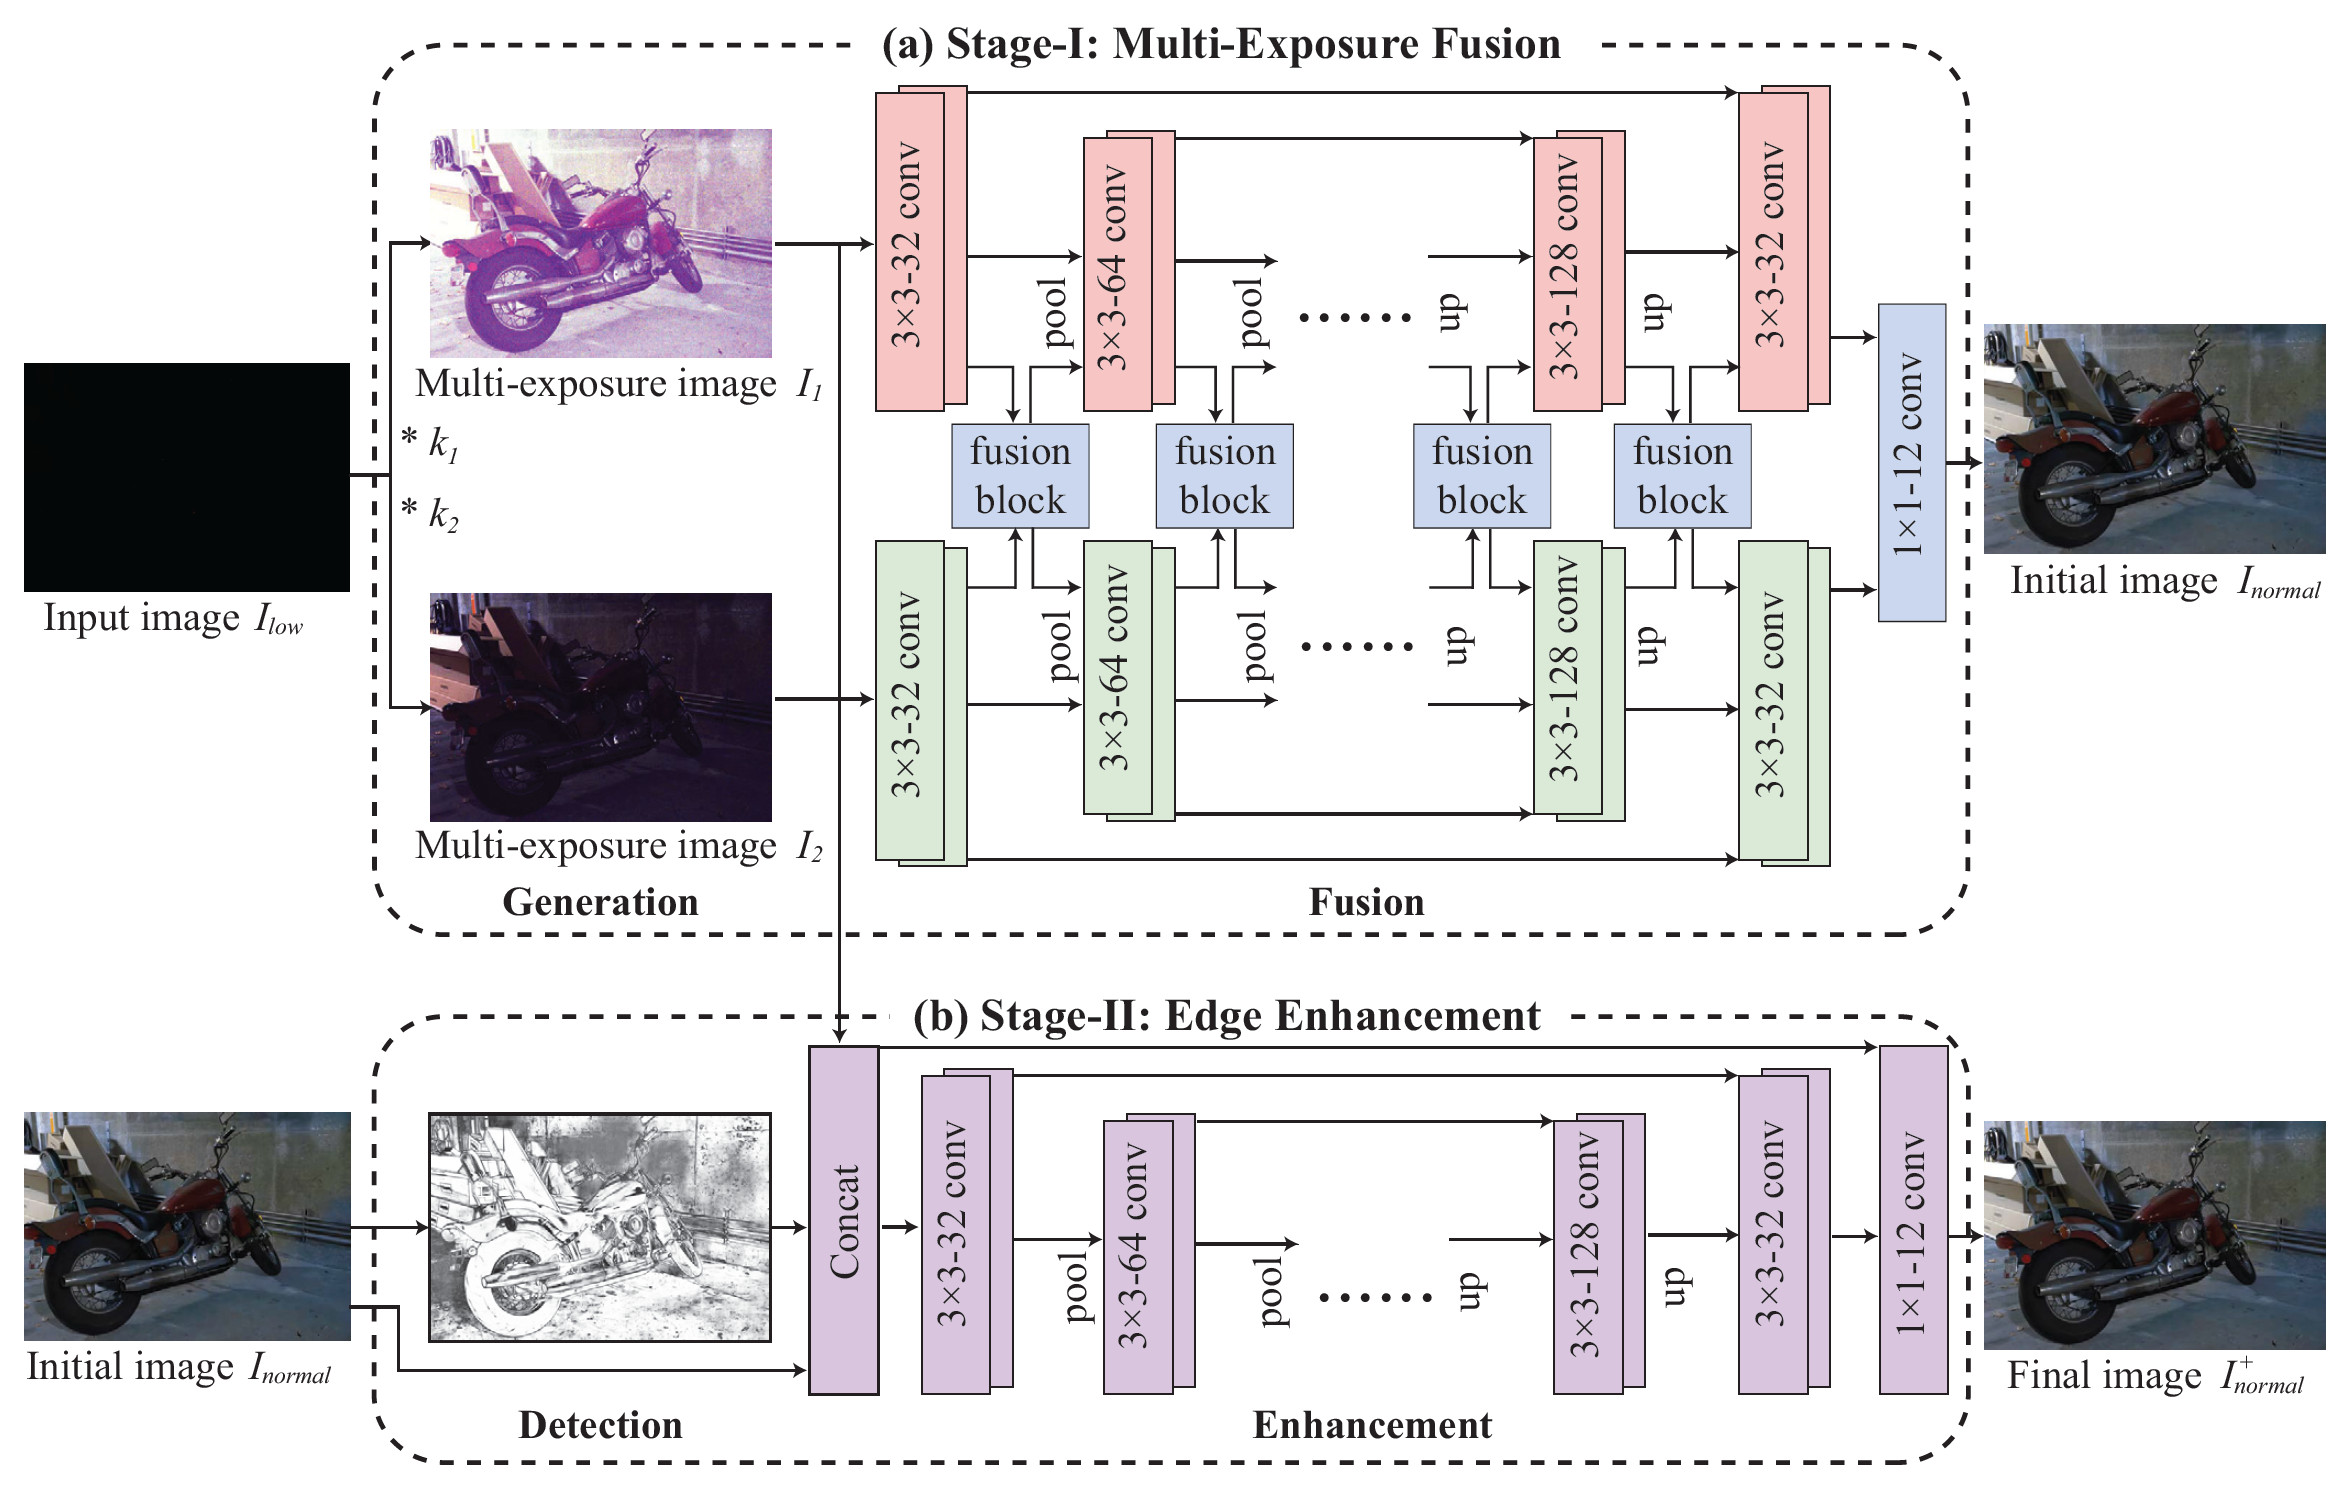
\includegraphics[width=\linewidth]{picture/LLIE/EEMEFN/EEMEFN framework}
			\captionsetup{font=scriptsize}
			\caption{\label{fig: EEMEFN}
				该 LLIE 结构源自\cite{zhu2020eemefn},如其 Multi-Exposure Fusion 部分采用多曝光融合结构,与由 Initial image 生成的边缘图进行 Concat, 后续通过一个 U-Net 网络进一步恢复图像。}
		\end{subfigure}
		\begin{subfigure}{0.45\columnwidth}
			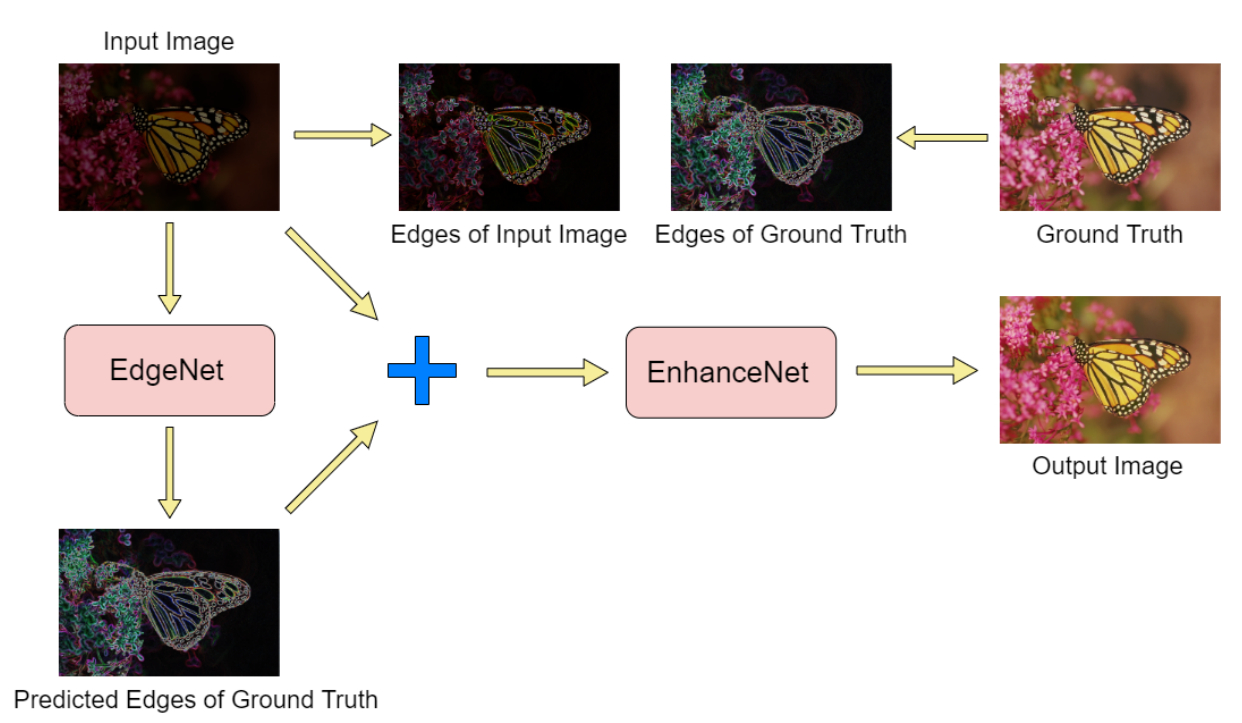
\includegraphics[width=\linewidth]{picture/LLIE/EdgeNet/Archtecture workflow}
			\captionsetup{font=scriptsize}
			\caption{\label{fig: EdgeNet} 
				该 LLIE 结构源自\cite{rana2021edge}使用 EdgeNet 首先从低光图像中过滤边缘,EnhanceNet 反复使用上采样和下采样块的组合,从局部到全局逐渐提取特征,并消除伪影和噪声。}
		\end{subfigure}
		\caption{
			\label{fig: Traditional Architecture}
			边缘图像指导弱光图像增强的传统架构。
		}
	\end{figure}
	
	\begin{figure}[htb]
		\centering 
		\begin{subfigure}{0.8\columnwidth}
			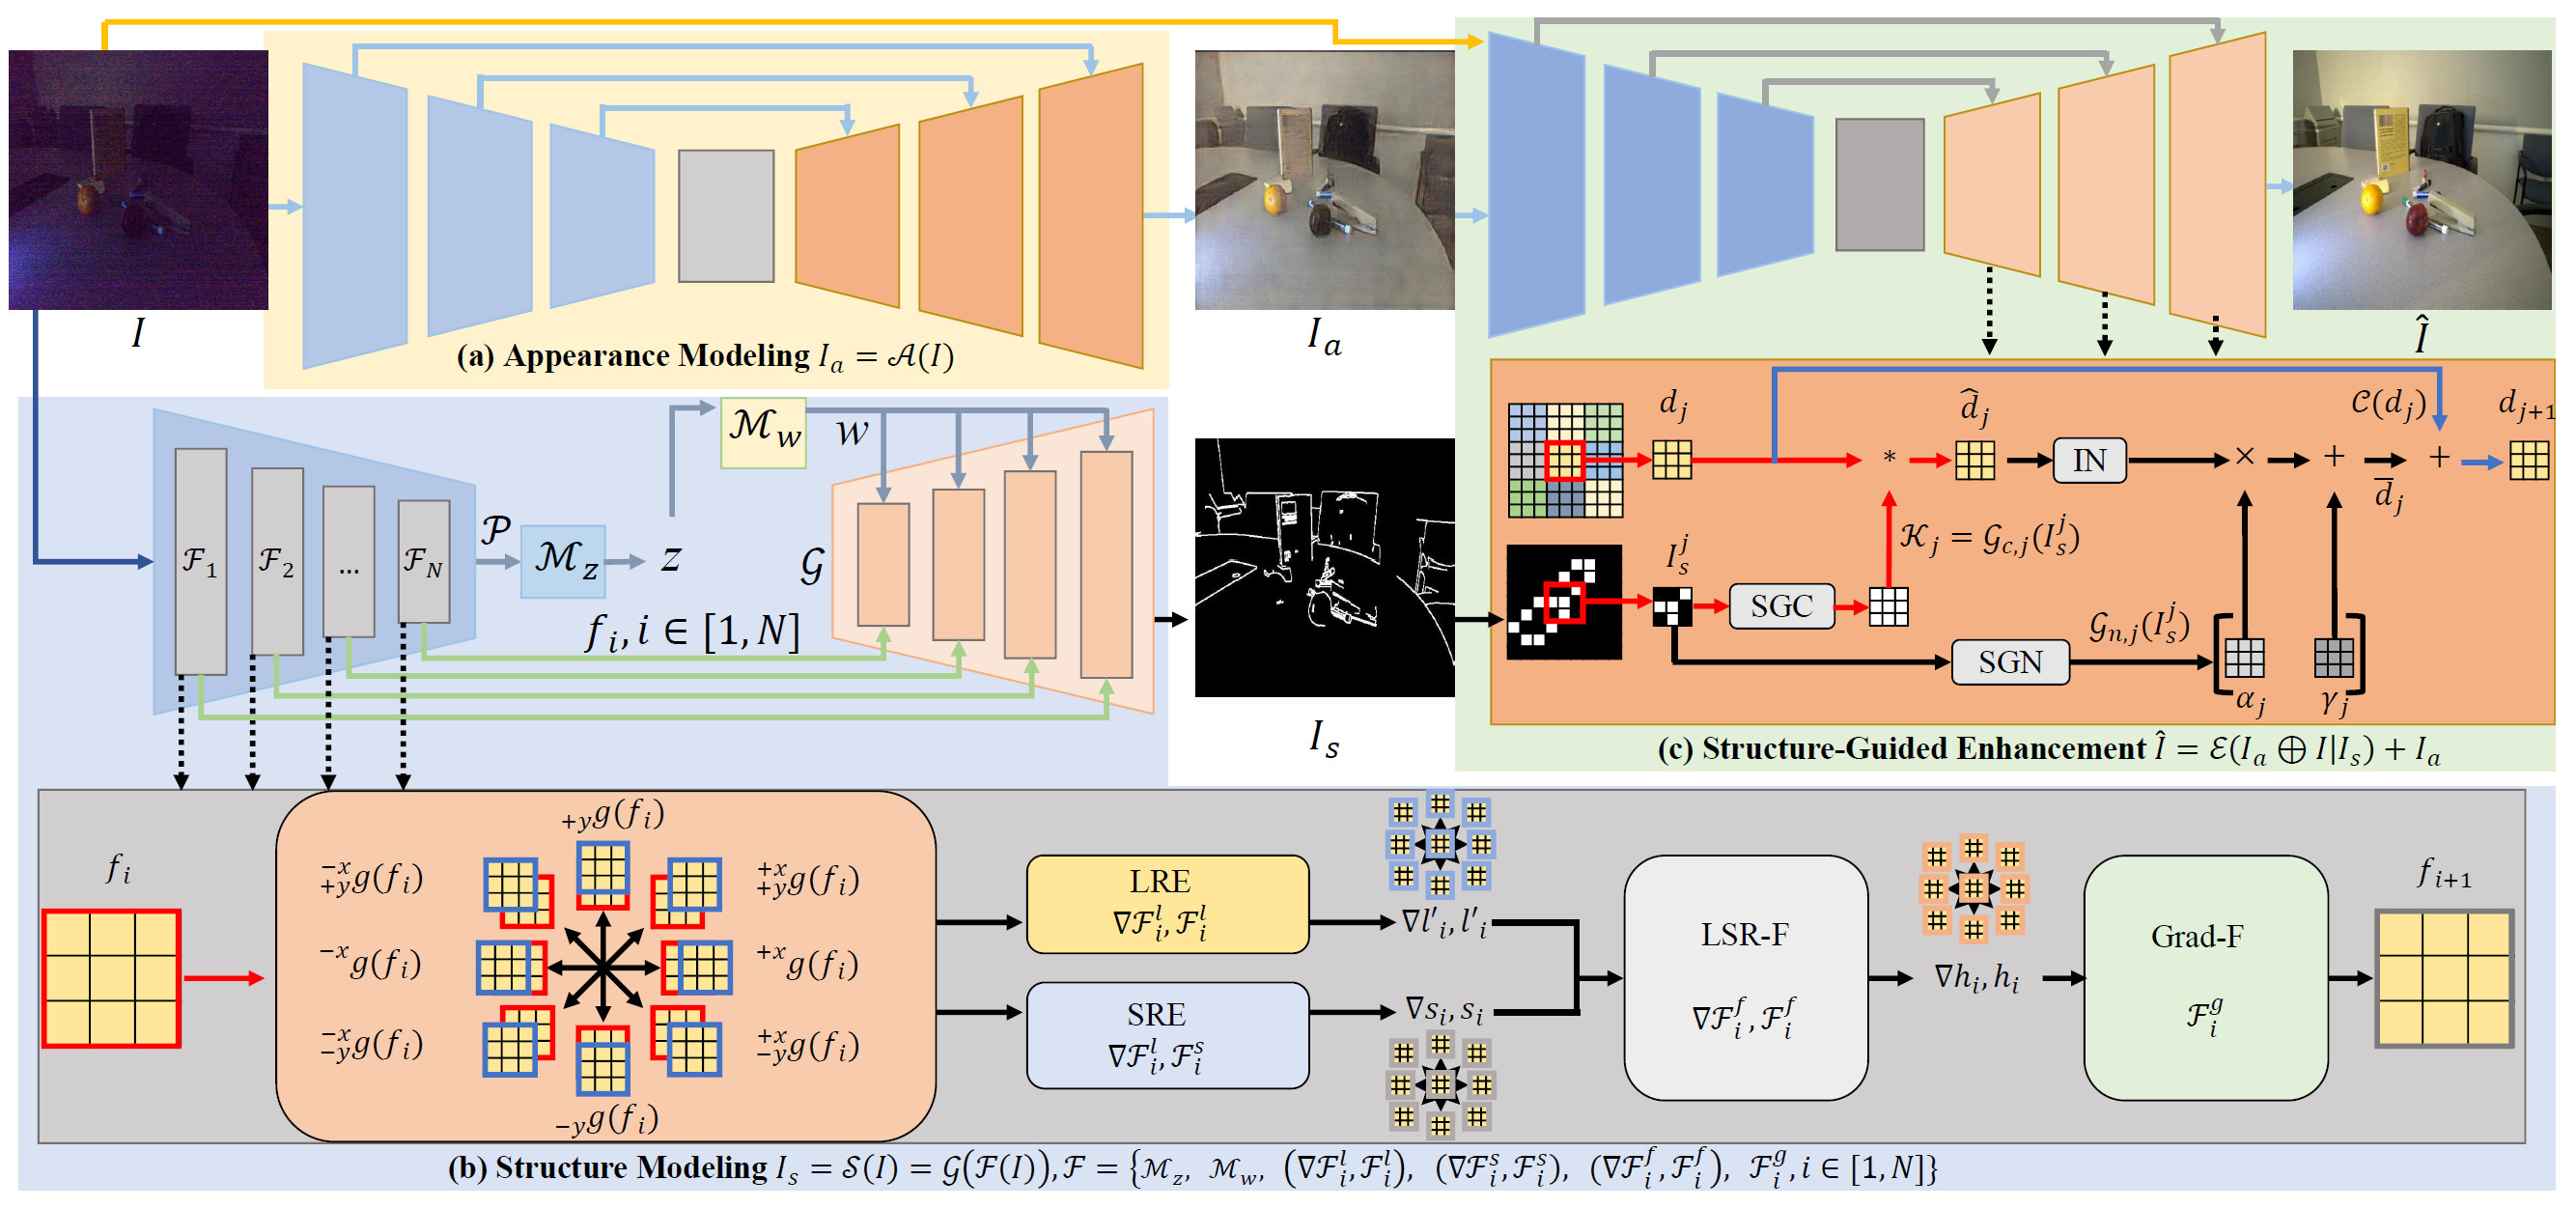
\includegraphics[width=\columnwidth]{picture/LLIE/Structure Modeling and Guidance/Overview}
			\captionsetup{font=scriptsize}
			\caption{该 LLIE 结构源自\cite{xu2023low},其提出一种基于 GAN Loss 的模型去对结构信息建模,通过获得的结构信息指导增强。}
			\label{fig: SMG-LLIE Architecture}
		\end{subfigure}
		\caption{
			\label{fig: SMG-LLIE Overview} 
			边缘图像指导弱光图像增强的最新架构(CVPR 2023)。
		}
	\end{figure}
	
	\begin{figure}[htb]
		\centering
		\begin{subfigure}{0.25\columnwidth}
			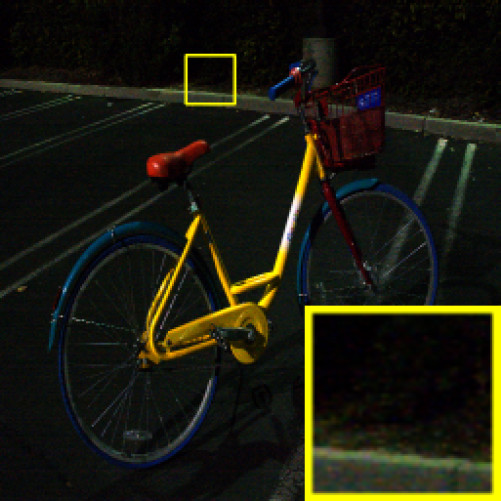
\includegraphics[width=\linewidth]{picture/LLIE/Structure Modeling and Guidance/Input}
			\captionsetup{font=scriptsize}
			\caption{Input}
			\label{fig: Input}
		\end{subfigure}
		\begin{subfigure}{0.25\columnwidth}
			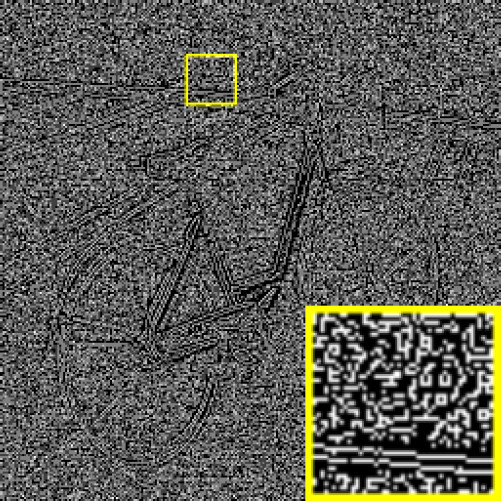
\includegraphics[width=\linewidth]{picture/LLIE/Structure Modeling and Guidance/Structure of (a)}
			\captionsetup{font=scriptsize}
			\caption{Structure of (a)}
			\label{fig: Structure of (a)}	
		\end{subfigure}
		\begin{subfigure}{0.25\columnwidth}
			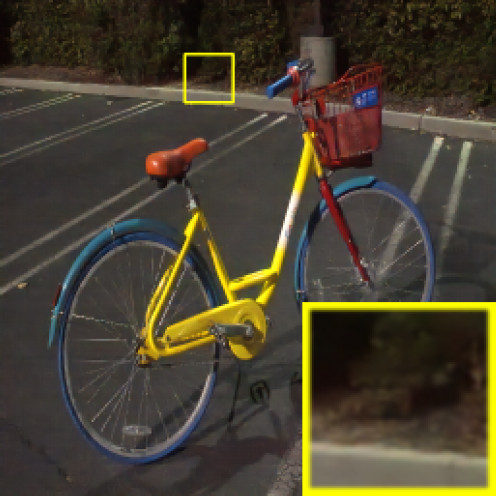
\includegraphics[width=\linewidth]{picture/LLIE/Structure Modeling and Guidance/SNR (CVPR 2022)}
			\captionsetup{font=scriptsize}
			\caption{SNR (CVPR 2022)}
			\label{fig: SNR (CVPR 2022)}	
		\end{subfigure}
		\begin{subfigure}{0.25\columnwidth}
			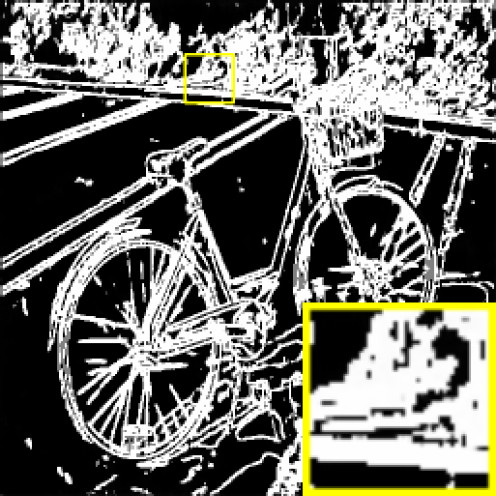
\includegraphics[width=\linewidth]{picture/LLIE/Structure Modeling and Guidance/Structure Modeling}
			\captionsetup{font=scriptsize}
			\caption{Structure Modeling}
			\label{fig: Structure Modeling}
		\end{subfigure}
		\begin{subfigure}{0.25\columnwidth}
			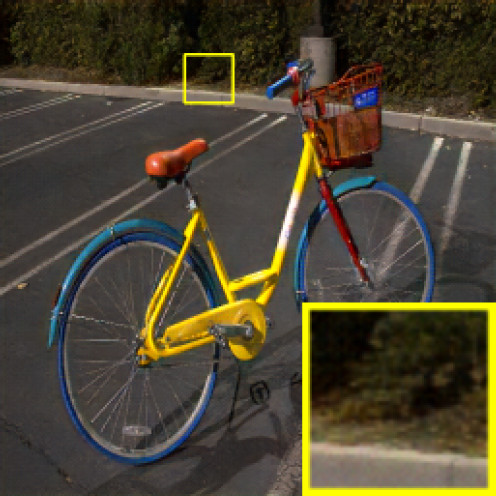
\includegraphics[width=\linewidth]{picture/LLIE/Structure Modeling and Guidance/Ours}
			\captionsetup{font=scriptsize}
			\caption{SMG-LLIE}
			\label{fig: SMG-LLIE}
		\end{subfigure}
		\begin{subfigure}{0.25\columnwidth}
			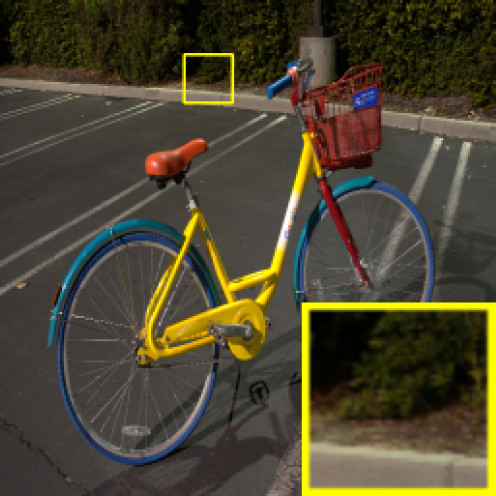
\includegraphics[width=\linewidth]{picture/LLIE/Structure Modeling and Guidance/Ground Truth}
			\captionsetup{font=scriptsize}
			\caption{Ground Truth}
			\label{fig: Ground Truth}
		\end{subfigure}
		\caption{
			\label{fig: Structural Information}
			SID-sRGB\cite{chen2018learning}中一张弱光图片, 通过SOTA方法 (c) 和\cite{xu2023low}提出的方法 (e)增强。作者的方法可以从输入的图像中合成结构图(d),使细节更清晰,对比度更清晰,颜色更鲜艳。虽然(c)的 PSNR 为 28.17,但其 SSIM 低为 0.75。作者的方法在dB和SSIM\cite{wang2004image}的得分都很高,分别为28.60 dB 和 0.80。
		}
	\end{figure}
	
	基于这个问题,即\textbf{如何更好的使用边缘图来“指导”弱光图像的恢复?}我们对此进行了相关文献调研。其中,一类方法(如图\ref{fig: Traditional Architecture}所示,我们称之为传统架构)是采用边缘检测思想来引导弱光图像增强,其策略是将边缘图与\textbf{一张从弱光中初步恢复的图像}(后面统一称作初步恢复图像)进行串联,然后通过一个增强网络来实现最终的图像增强\cite{zhu2020eemefn, rana2021edge}。但是我们通过观察这类模型的架构发现其具有以下三个特点:
	
	\begin{itemize}
		\item [(1)] 其恢复结果的质量往往会受到最后的增强网络设计和初步恢复图像所包含特征与真实图像特征之间的相似度的影响。
		
		\item [(2)] 边缘图的准确性会极大影响最终的恢复结果,直接从弱光图像中获取边缘图具有一定的挑战性。
		
		\item [(3)] 边缘图与初步恢复图像之间多采用串联方式输入卷积以获得最终增强结果。
	\end{itemize}
	
	传统架构存在一定的局限性,虽然采用了边缘结构信息增强弱光图像,但是无法很好的利用边缘信息语义指导恢复弱光图像,需要在现有的直接串联方法的基础上进行改进。此外,从低光照中的图片很难提取到好的结构信息,如何设计更好的边缘网络从弱光图像中提取出接近 GT 边缘图的结果是我们需要考虑的问题。
	
	作者\cite{xu2023low}提出了一种基于结构先验的图像增强方式,以更好的从弱光图像中提取到更有效的边缘信息并用于指导图像增强。从图\ref{fig: Structural Information}和\ref{fig: LLI Structure Information}中可以看到边缘图和LBP图\cite{pietikainen2010local}所反映结构信息具有明显的区别,边缘信息能反映更多的细节信息。我们不难发现,相较于LBP,图像边缘图仅保留了很少的数据量,其剔除了不相关的信息,保留了图像重要的结构属性。人类视觉系统对边缘高度敏感,保留结构信息对图像重建任务的性能至关重要。定义边缘可以通过学习区分黑暗区域的不同物体来指导增强过程,而不仅仅是识别低光区域。通过保留图像中的结构属性,这使得物体之间的可见性更好。
	
	综上所述,本研究旨在实现以下明确的研究目标\footnote{在对Xu等人\cite{xu2023low}的模型(参见图\ref{fig: SMG-LLIE Architecture})进行深入分析后,本研究旨在通过采用与原作者不同的方法论来实现若干具体目标,并力求在关键评价指标上超越原模型的性能。具体而言,本研究的核心目标包括:首先,在目标(1)和目标(2)的框架内,探索与Xu等人不同的优化策略;其次,这些优化策略应致力于提升模型的整体性能,目的在于在关键评价指标上实现超越原作者的成果。通过这种方法,本研究不仅旨在增强现有模型的能力,同时也寻求对该领域的理论和实践知识做出贡献。}:
	
	\begin{itemize}
		\item [(1)] \textbf{边缘网络的开发:} 设计并构建一个创新的边缘网络,其核心功能是从低光照图像中直接提取边缘结构图。该网络生成的结构图应与地面真实(GT)生成的边缘结构图具有高度的相似性,从而确保准确性和可靠性。
		
		\item [(2)] \textbf{初步恢复图像的生成模型:} 开发一个用于生成初步恢复图像的低光照图像增强模型。该模型应专注于从弱光条件下的图像中恢复清晰度和细节,以提高整体图像质量。
		
		\item [(2)] \textbf{边缘语义信息的增强网络模型:} 在现有的直接串联方法基础上,进行创新性改进,构建一种更有效利用边缘语义信息的增强网络模型。目的在于通过这种改进,进一步提升图像增强过程中边缘结构的利用效率和效果。
	\end{itemize}
	
	通过实现这些目标,本研究期望对低照度图像处理领域的理论与实践作出贡献,特别是在图像边缘结构的提取和利用方面。
	
	\part*{研究内容}
	
	\section{采用的方法}

	\subsection{注意力机制}
	
	在计算机视觉领域,研究人员往往会使用不同类型的注意力机制,目的是使模型聚焦于图像本身。这大致分为两种类型:一种是基于通道的注意力机制,即 Squeeze-and-Excite。另一个是基于空间的注意力机制\cite{woo2018cbam}。然而,研究发现这些类型有三个局限性:
	
	\begin{itemize}
		\item[(1)] 
		卷积捕捉远距离特征的能力较差;
		
		\item[(2)]
		注意力机制关注所有输入;当分辨率较大时,计算成本增加;
		
		\item[(3)]
		不同时关注通道和空间维度关注信息。这就造成了信息的浪费和注意力的减弱。
	\end{itemize}	
	
	针对第一个限制 \cite{ramachandran2019stand} 将所有卷积替换为独立的自注意层和空间意识的独立自注意层,替换后的模型为纯注意模型。纯注意模型增强了网络对远距离特征连接的建模能力。在 ImageNet分类任务和 COCO 对象检测任务中,该模型优于使用卷积的基线模型。对于第三个限制,Woo 等人\cite{woo2018cbam}提出了一种卷积块注意模型 CBAM,这是一种轻量级的通用注意模型。该模型从通道维度和空间维度两方面关注重要信息。由于 CBAM 从多个维度提取重要信息,该模型被广泛应用于目标检测、目标分类等任务。实验表明,CBAM 模块可以显著提高网络的表达能力。同时,CBAM 可以搭配 SCConv\cite{li2023scconv}结构,SCConv 是一种名为可以即插即用的卷积模块,目的是减少卷积神经网络中特征之间的空间和通道冗余,从而压缩 CNN 模型并提高其性能。
	
	\subsection{U-Net网络结构}
	
	U-Net 网络由卷积层、下采样、上采样和跳过连接操作组成,其编码器和解码器具有对称结构。长期以来,U-Net 网络及其改进结构由于其强大的特征学习和特征重构能力,在图像语义分割领域取得了巨大的成功。U-Net 网络在弱光图像增强方面显示出出色的效果。Chen 等\cite{chen2018learning}创新性地提出了一种基于 U-Net 框架的弱光图像增强网络。该网络的核心架构是多尺度上下文聚合网络 (CAN) 和 U-Net 网络。之后的工作\cite{chen2018learning, zamir2021learning}也将 U-Net 架构应用到自己的网络中,其网络包含两个子网。即图像约简子网和感知损失子网,其中图像约简子网具有与\cite{chen2018learning}相同的 U-Net 架构。虽然\cite{chen2018learning, zamir2021learning}在使用U-Net架构增强图像方面取得了一定的效果,但\cite{meng2020gia}认为\cite{chen2018learning, zamir2021learning}网络忽略了全局信息,导致增强图像中的颜色不自然和物体伪影问题。为了改善以往网络的缺陷,利用 U-Net 架构,\cite{meng2020gia}在U-Net的编码器和解码器之间增加了全局信息感知模块(global information awareness module, GIA), GIA 可以将全局信息整合到整个网络中,改善增强图像中的颜色不一致和伪影。经过对\cite{chen2018learning, meng2020gia, zamir2021learning}的仔细研究,基于 U-Net 网络的弱光图像增强方法取得了很好的效果。然而,该网络仍然存在两个局限性:
	
	\begin{itemize}
		\item[(a)] 
		跳过连接只融合相同尺度的特征,导致编码器和解码器之间存在较大的语义差距;
		
		\item[(2)]
		全局上下文信息的连接相对稀缺。
	\end{itemize}	
	
	这两个限制容易导致增强图像的细节丢失、对比度差和颜色信息不准确。Zhou等\cite{zhou2018unet++,zhou2019unet++}改进了 U-Net 架构生成 U-Net++,在 U-Net++ 中将跳跃连接重新设计为一系列嵌套的密集跳跃连接,实现了多个特征的融合,加强了不同层次的特征信息接触。
	
	\subsection{CNN网络结构}
	
	CNN 在许多计算机视觉任务中表现出了令人印象深刻的结果。CNN 利用注意力机制\cite{yang2021locally, zhang2020attention}和上下文信息,从原始图像中生成注意感知并提取多尺度特征\cite{li2018multi,zamir2020learning}。基于 CNN 的低光图像增强方法不断发展。例如,基于 CNN 的自适应弱光图像增强框架\cite{li2020visual}极大地增强了图像对比度、颜色和细节信息。然而,现有的基于 CNN 的方法大多侧重于图像亮度、纹理和颜色的恢复\cite{xu2020learning}。由于局部光照不均匀,颜色信息和细节信息丢失严重,容易出现过增强或增强不足的问题。
	
	\subsection{Transformer网络结构}
	
	Transformer架构\cite{vaswani2017attention}在图像处理领域的应用以来\cite{dosovitskiy2020image},其在捕获全局特征方面的能力已经引起了行业的广泛关注。然而,在图像复原任务中,由于Transformer基于自注意力机制的计算特性,其面临着较高的计算复杂度问题。这一挑战通常需要通过改进前馈神经网络(FFN)来解决,以便更有效地捕获关键信息,从而增强模型的非线性建模能力\cite{wang2022ultrahighdefinition}。为了缓解计算负担,部分研究工作尝试采用局部窗口策略来限制自注意力机制的计算范围,并借鉴 U-Net 架构,引入跳过连接机制以增强特征传递\cite{wang2021uformer}(如图\ref{fig: Uformer}所示)。尽管这种方法在降低计算成本方面取得了一定成效,但它可能会削弱Transformer架构在捕获图像中长距离特征的能力,进而影响其在图像复原任务中的整体性能。为了克服这一限制,提出的解决方案\cite{chen2023cross}主要集中在窗口间的交互和与卷积神经网络(CNN)模块的耦合上。这种方法旨在将CNN的平移不变性和局部性归纳偏差融入Transformer架构中,从而实现两者优势的互补。我们将这类解决方案称为CNN与Transformer的串联策略。
	
	\begin{figure}[htb]
		\centering 
		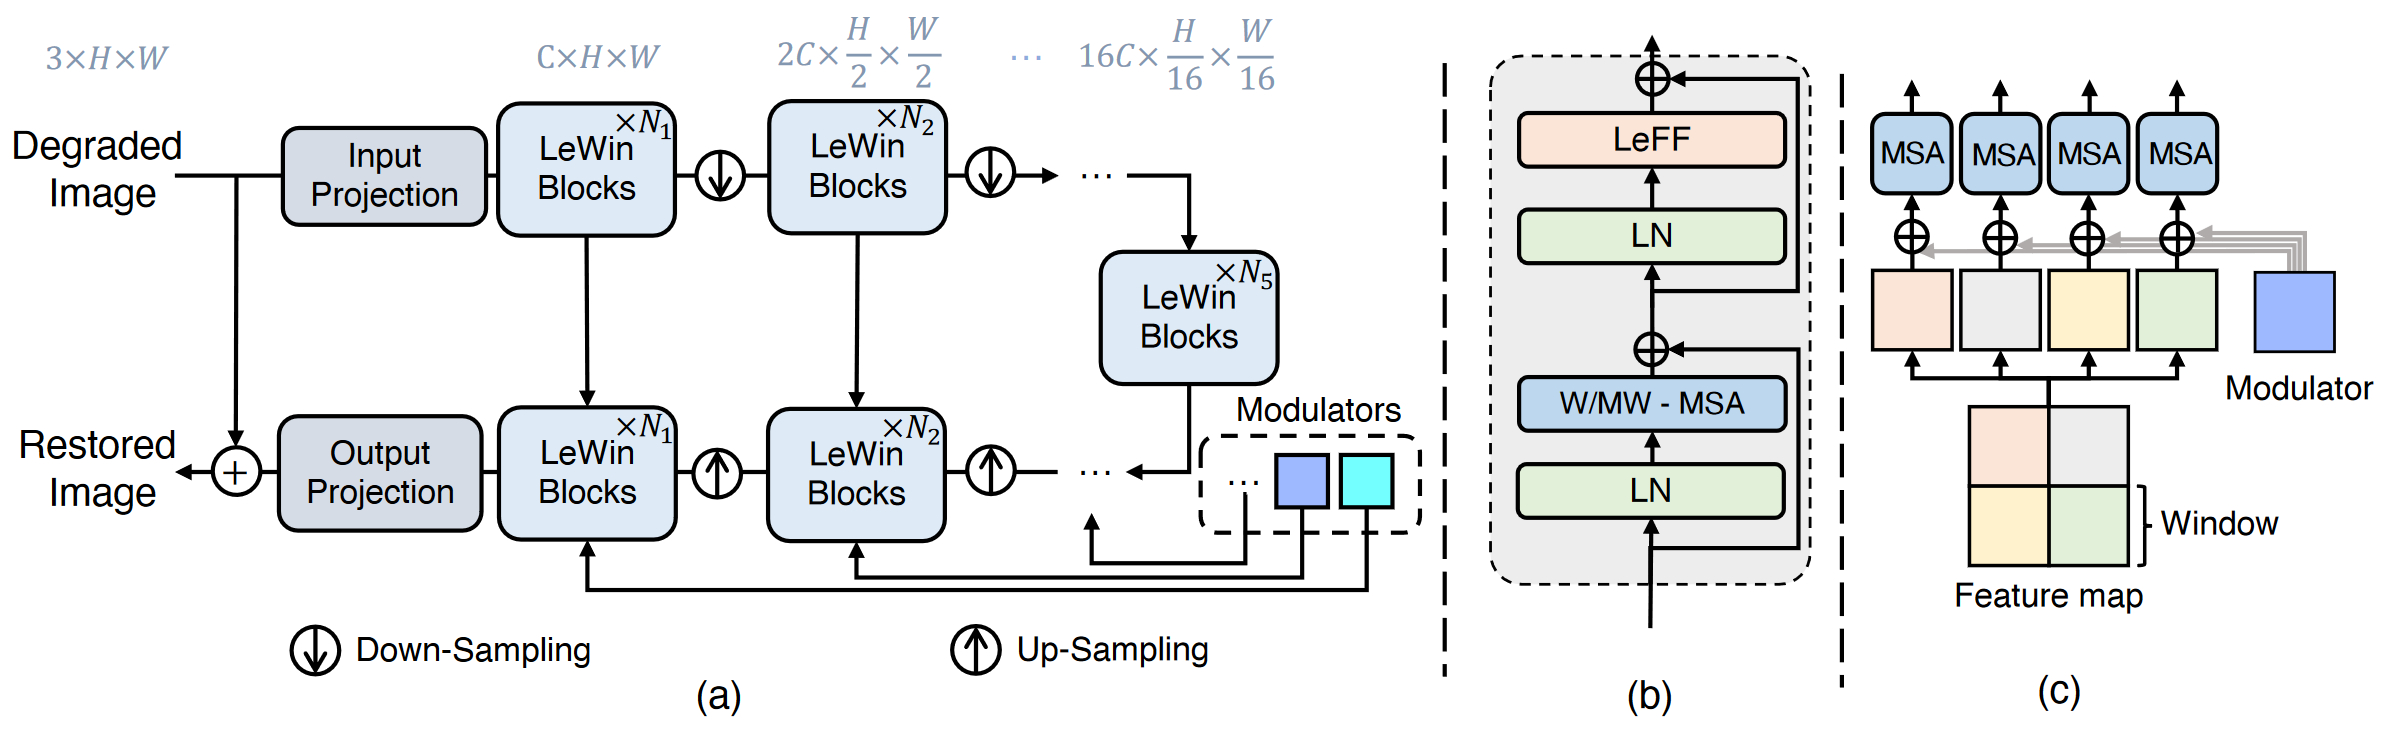
\includegraphics[width=\columnwidth]{picture/LLIE/Uformer/Uformer}
		%\captionsetup{font=scriptsize}
		\caption{
			\label{fig: Uformer} 
			Uformer 的结构。
		}
	\end{figure}
	
	\section{具体的方法}
	
	\subsection{初步恢复图像的生成模型}
	
	\textbf{初步恢复图像的生成模型}目前主要包括以下几种:
	
	\begin{itemize}
		\item[(1)] 
		利用多曝光技术(Multi-exposure image fusion, MEF)\footnote{多曝光技术已被实验证明可以有效的解决 LLIE 任务中普遍存在的色彩失真问题。}获得具有不同曝光度的图像,然后结合恢复网络进行初步恢复\footnote{常见的架构如基于 GAN 的多曝光图像融合架构,基于端到端深度学习框架下多曝光图像融合算法,基于稀疏表示和可平移复方向金字塔变换的多曝光融合框架。}\cite{burt1984pyramid};
		
		\item[(2)]
		结合 CNN 和 Transformer 架构的方法,可以是类似于 Uformer \cite{wang2022uformer}的串行架构,亦或者是类似于 Conformer 的并行架构。我们提出的 CNN 和 Transformer 并行架构(见图\ref{fig: First Architecture})。
		
		\item[(3)]
		通过 U-Net 进行弱恢复。
		
	\end{itemize}	
	
	但由于噪声和伪影的存在,以及色彩与真实图像之间的差异,直接采用神经网络恢复结果通常并不理想。
	
	\begin{figure}[htb]
		\centering 
		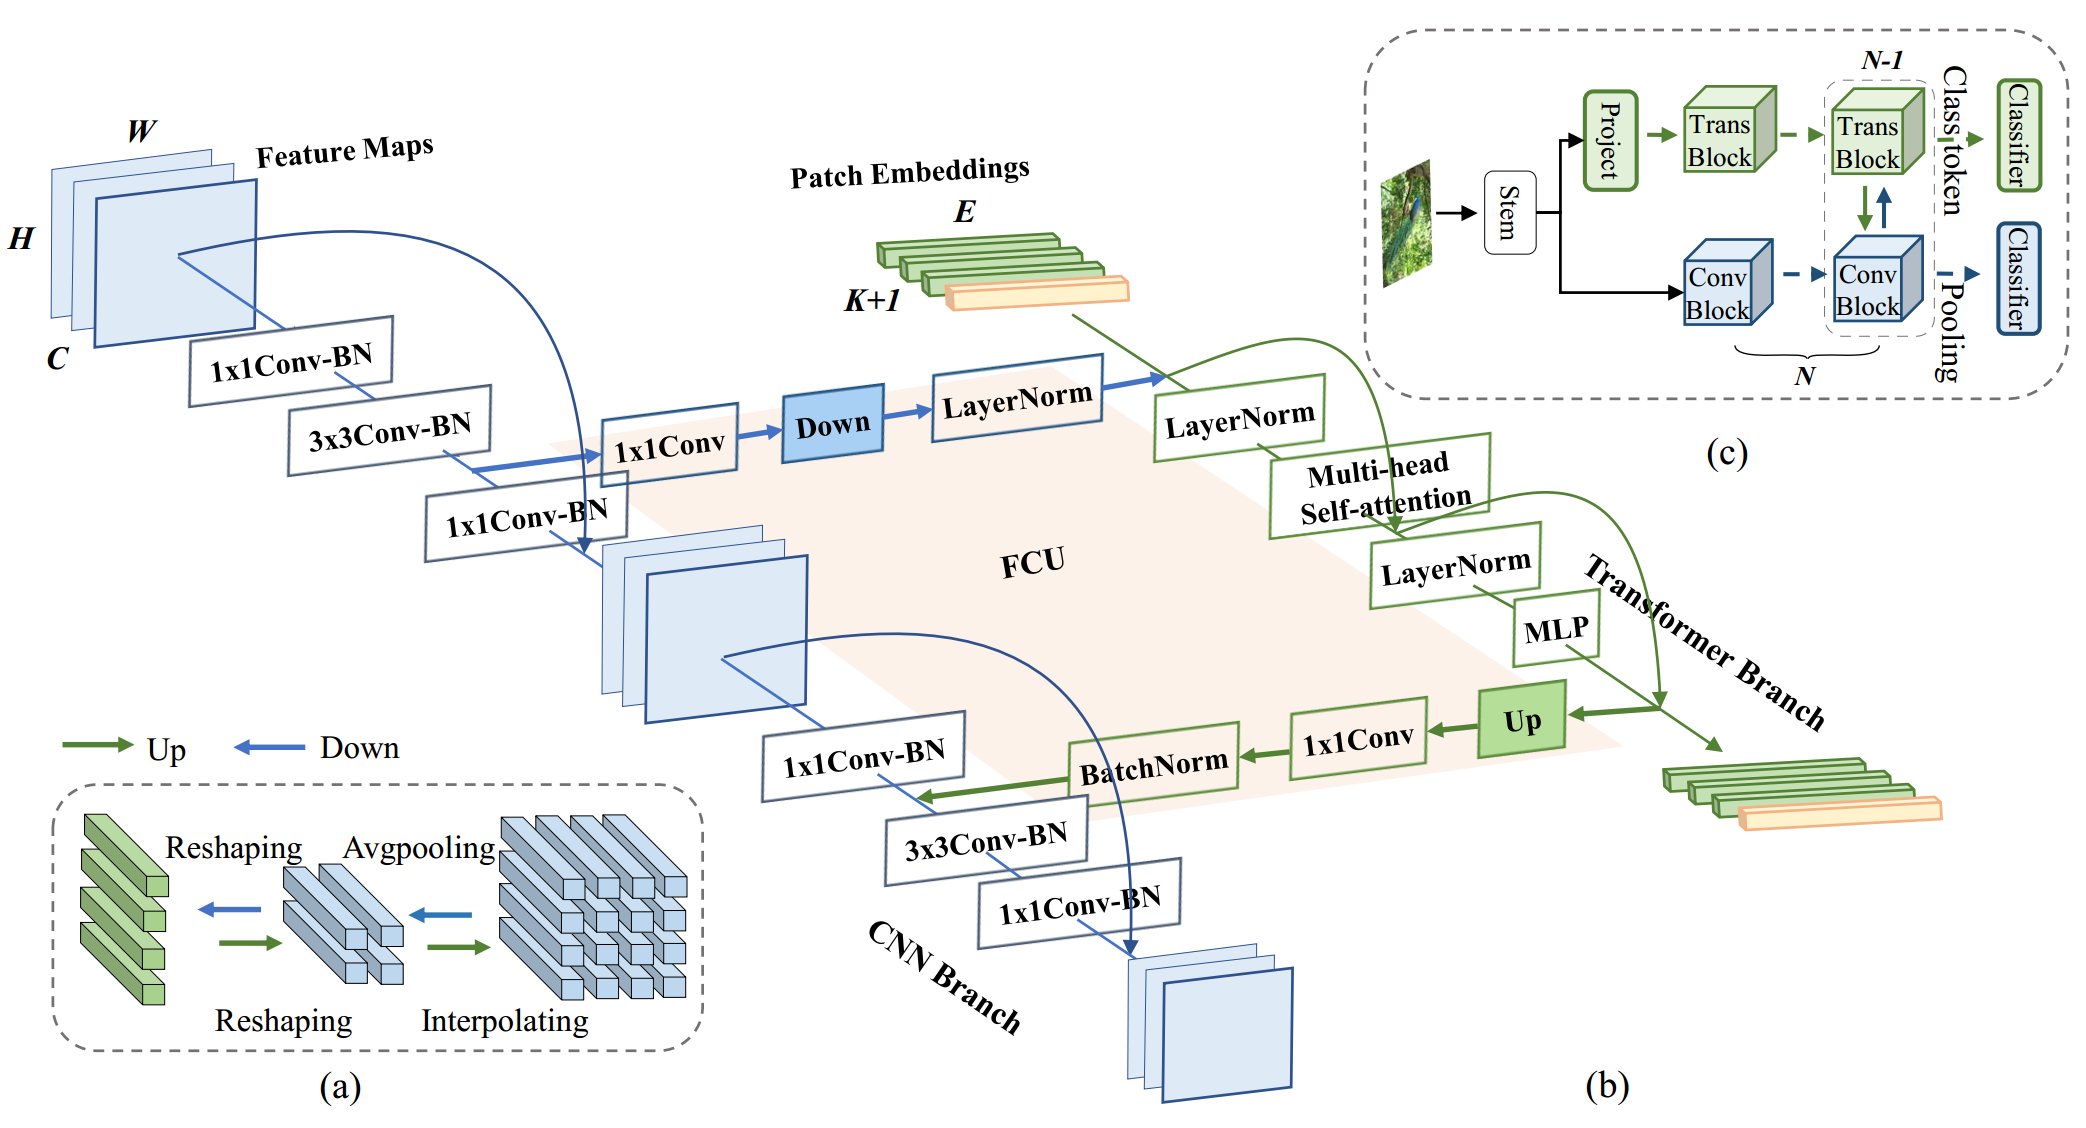
\includegraphics[width=0.9\columnwidth]{picture/LLIE/Conformer/the proposed Conformer}
		\caption{
			\label{fig: Conformer} 
			作者\cite{peng2021conformer}提出的网络结构。(a) 特征图和补丁嵌入用于空间对齐的上采样和下采样。(b) CNN块、Transformer块和特征耦合单元(FCU)的实现细节。(c) 缩略图。 
		}
	\end{figure}
	
	在计算机视觉领域,图像特征的研究通常聚焦于两个主要方面:局部特征和全局特征。局部特征,也称为短距离特征,指的是对图像中微小区域的紧凑向量描述,这些特征在众多计算机视觉算法中扮演着基础角色\cite{jain1991unsupervised, lowe2004distinctive, ojala2002multiresolution}。相对而言,全局特征,或长距离特征,涵盖了更广泛的范围,包括但不限于长距离轮廓\cite{lisin2005combining}、形状描述符以及不同对象类别的识别。
	
	在深度学习的框架下,卷积神经网络(CNN)通过分层的卷积操作,逐步提取并加工图像的局部特征。这些特征随后被保留在特征图中,以供后续处理和分析。另一方面,视觉变换器(Vision Transformers)则采用一系列自注意力模块,这些模块能够以更加灵活的方式聚合这些特征,从而形成对整体图像的全面和全局性理解。这种方法在处理图像的全局特征时显示出了显著的优势,尤其是在捕获长距离依赖关系和整体图像结构方面。
	
	\begin{figure}[htb] 
		\centering 		
		\begin{subfigure}{\textwidth}
			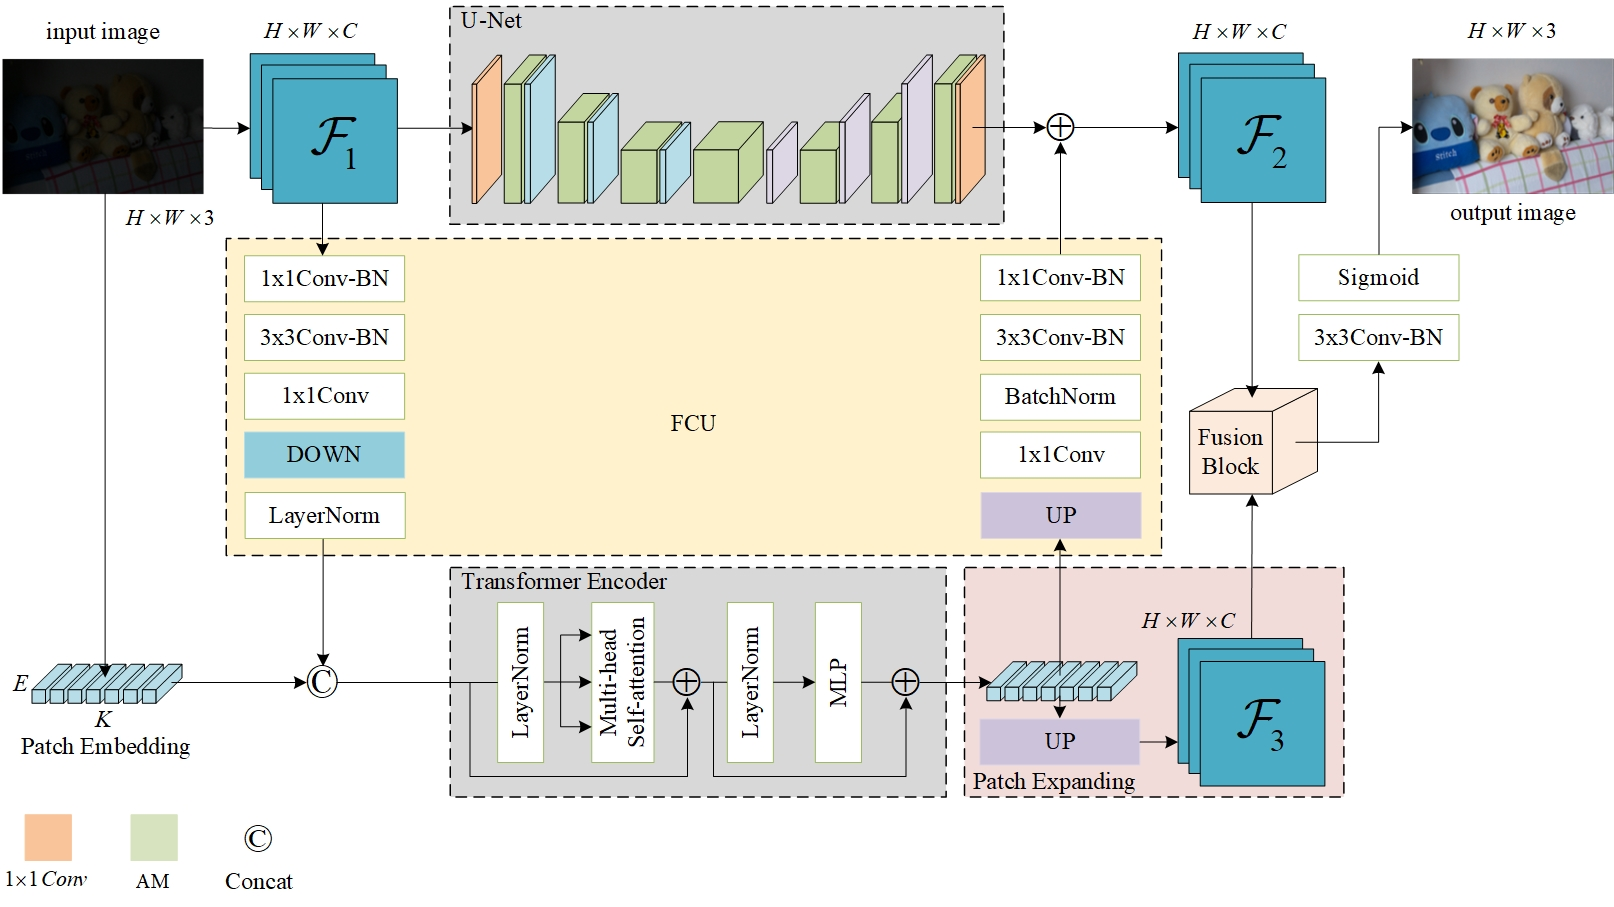
\includegraphics[width=\linewidth]{picture/LLIE/My Architecture/The proposed initial architecture.jpg}
			\captionsetup{font=scriptsize}
			\caption{Parallel Architecture}
			\label{fig: First Architecture}
		\end{subfigure}\\
		\begin{subfigure}{0.4\textwidth}
			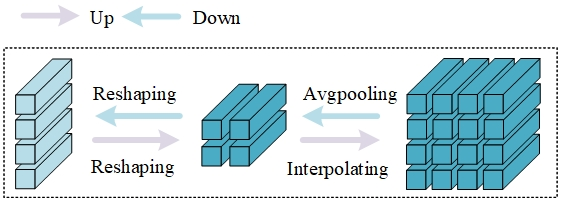
\includegraphics[width=\linewidth]{picture/LLIE/My Architecture/Up-sampling and down-sampling}
			\captionsetup{font=scriptsize}
			\caption{Up-sampling and Down-sampling}
			\label{fig: Up-sampling and down-sampling}
		\end{subfigure} \
		\begin{subfigure}{0.4\textwidth}
			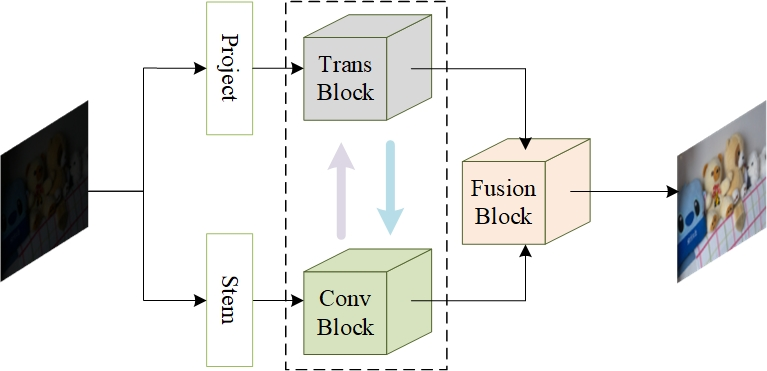
\includegraphics[width=\linewidth]{picture/LLIE/My Architecture/The proposed initial architecture(Abstract Picture)}
			\captionsetup{font=scriptsize}
			\caption{Thumbnail of PACUT}
			\label{fig: The proposed initial architecture(Abstract Picture)}	
		\end{subfigure}
		%\captionsetup{font=scriptsize}
		\caption{
			\label{fig: PACUT}
			我们提出的初步恢复图架构。图\ref{fig: First Architecture} CNN 分支和 Transformer 分支以及 FCU (Feature Coupling Unit)。图\ref{fig: Up-sampling and down-sampling} 特征映射和 Patch embeddings 空间对齐的上采样和下采样过程。 图\ref{fig: The proposed initial architecture(Abstract Picture)} PACUT 的缩略图。PACUT 结构受 Conformer\cite{peng2021conformer}启发,将原来结构中 CNN 分支的 ResNet 结构修改为 U-Net 结构。其采用一个 U-Net 和 ViT 的并行架构,通过 U-Net 结构得到一个弱恢复的弱特征图 $\mathcal{F}_2$,通过 ViT 融合的特征可以初步增强弱特征图 $\mathcal{F}_2$,ViT 的输出经过 Patch Expanding 的特征图 $\mathcal{F}_3$ 经过与 U-Net 输出的特征图 $\mathcal{F}_2$ 融合之后得到一个初步恢复的图片 output image,用以后续参与图片的进一步恢复。
		}
	\end{figure}
	\FloatBarrier
	
	在初步恢复图的生成方面,我们受到了 Conformer 结构\cite{peng2021conformer}(如图)的启发,该结构巧妙地结合了卷积神经网络(CNN)在捕获短距离特征\cite{jain1991unsupervised, lowe2004distinctive, ojala2002multiresolution}方面的优势与Transformer自注意力模块在捕获长距离特征\cite{lisin2005combining}依赖关系方面的能力。然而,Transformer的自注意力模块在捕获远距离特征的同时,可能会忽视局部特征的细节。为了克服这一局限性,Conformer结构融合了卷积运算和自注意力机制,以增强表示学习的能力。为了最大限度地利用局部特征和全局表征的互补优势,我们提出一种新颖的并行深度学习架构(如图\ref{fig: PACUT}所示),专门针对低光照条件下的图像增强问题。该模型融合了经典的 U 型网络和 Transformer 深度学习方法,旨在提升弱光图像增强任务中恢复图像的可视性和质量,同时保留关键的细节和纹理\cite{karu1996there}信息。
	
	具体而言,该架构由两个并行分支、一个 Stem 模块、一个特征连接单元(FCU, Feature Coupling Unit)以及一个为两个分支设计的融合模块(Fusion Block)组成。Stem模块\footnote{Stem模块一般包含几个卷积层、激活函数、池化层(如最大池化或平均池化)等。这些组件共同工作,以有效地提取和转换输入数据的特征,为网络的后续层提供更加丰富和有用的信息。}由 VGG16 网络的前四层构成\cite{szegedy2016rethinking},截至第一个最大池化层,其主要功能是提取图像的初始局部特征,如边缘和纹理等,随后将这些特征输入到 CNN 分支。CNN 分支采用了改进的 U-Net 网络结构,而 Transformer 分支则由一个经过修改的 Vision Transformer 构成,去除了分类功能,仅保留特征提取功能。
	
	在这种并行结构中,CNN分支和Transformer分支分别专注于最大程度地保留局部特征和全局表征。FCU作为一种桥接模块,其作用是融合CNN分支中的局部特征和Transformer分支中的全局表征,如图\ref{fig: First Architecture} 所示。FCU从第二步开始应用,因为两个分支的初始特征虽相同,但表征形式不同。在整个网络中,FCU通过双向交互融合特征图和Patch Embeddings。
	
	最终,两个分支的特征都被送入特征融合模块进行处理。对于Transformer分支,为了更有效地利用长距离特征,我们在进行Patch Expanding操作之前,通过FCU与CNN分支进行融合。最后,两个分支的输出通过特征融合模块处理后,生成最终的增强图像。在训练过程中,我们采用了结合$\mathcal{L}_1$和SSIM损失函数的策略,以优化模型在像素级误差和感知质量方面的表现。
	
	\subsubsection{CNN 分支}
	
	在PACUT架构中,CNN分支基于U-Net网络结构,这是一种原本为图像分割任务设计的网络架构,但其在图像增强领域同样展现出卓越的性能。U-Net的显著特点在于其对称的编码器-解码器结构和编码器与解码器之间的跳跃连接。在本研究中,CNN分支的目标是从输入的低光照图像(LLI)中提取丰富的特征,包括边缘、纹理、颜色和亮度信息,并最终生成增强的图像(EI)。
	
	\begin{figure}[htb]
		\centering 
		\setlength{\abovecaptionskip}{-1.5cm}
		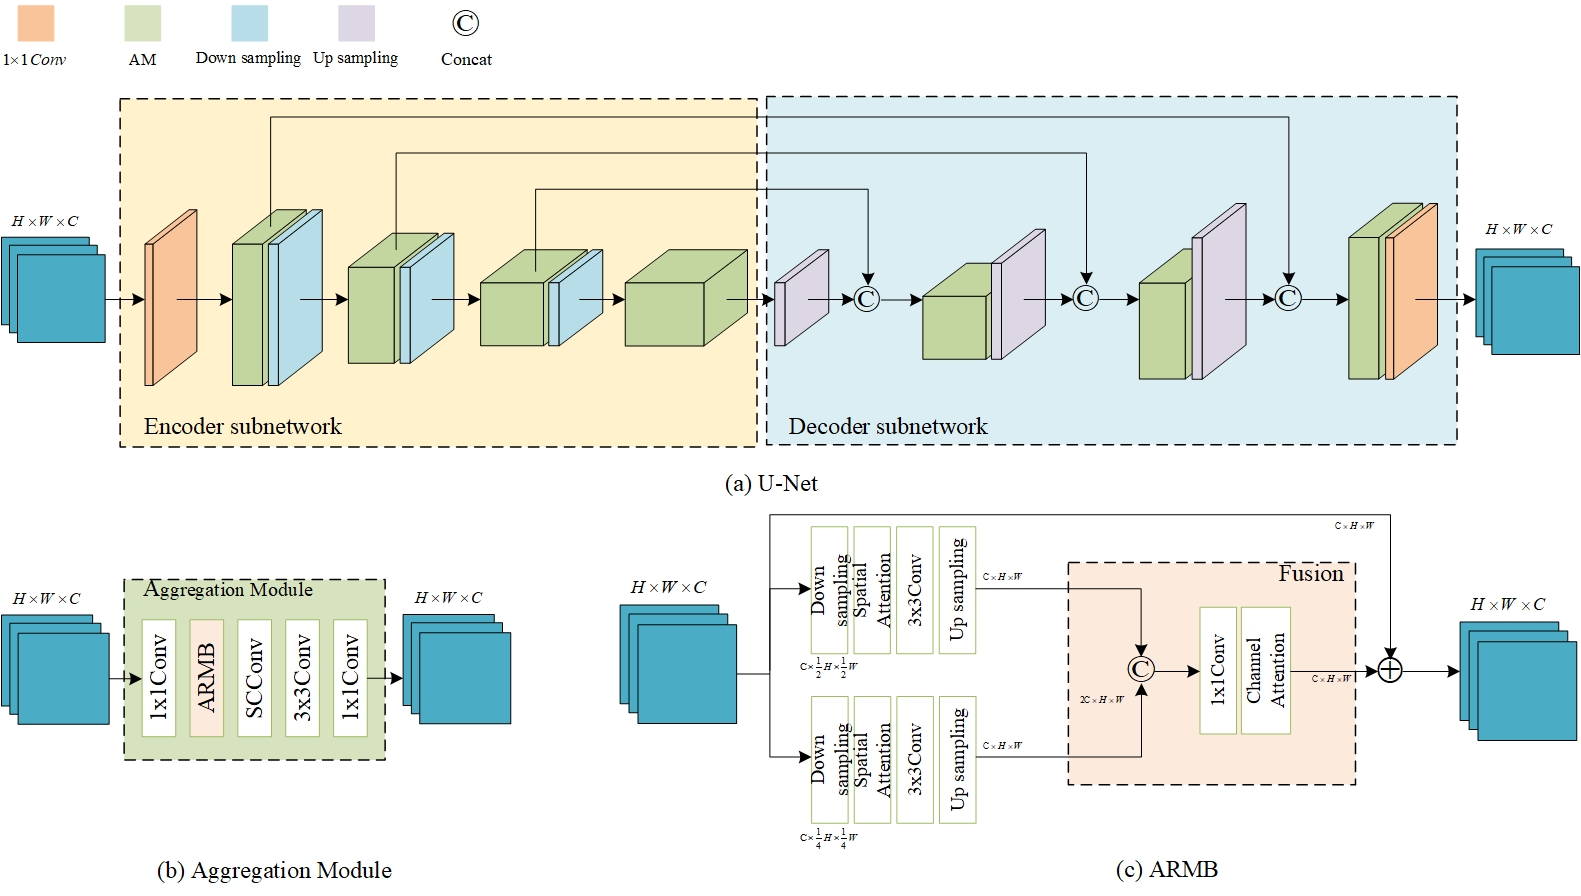
\includegraphics[width=\columnwidth]{picture/LLIE/My Architecture/U-Net and AM}
		%\captionsetup{font=scriptsize}
			\caption{
				\label{fig: U-Net and AM} 
				CNN分支及其所属的模块。
			}
	\end{figure}
	
	针对低光照图像增强任务,我们设计了 UNetEnhance 模型,用于CNN分支。该模型在经典 U-Net 架构的基础上进行了多项改进,以增强其处理低光照环境下图像的能力。这些改进包括更深的网络结构、改进的特征融合机制和高效的信息传递路径。UNetEnhance模型的结构如图\ref{fig: U-Net and AM}所示,它由两部分组成:1) 编码器子网络(Encoder Subnetwork)和2) 解码器子网络(Decoder Subnetwork)。编码器子网络采用了多层卷积网络结构,在每层中集成了空间注意力机制和通道注意力机制\cite{woo2018cbam}。与传统 U-Net 相比,这种设计增加了网络的深度,使其能够捕获更丰富的特征信息。解码器部分则采用了上采样和卷积操作,逐步恢复图像的空间分辨率,并引入了改进的特征融合策略,将编码器中的低级特征与解码器的高级特征有效结合,以更好地重建图像细节。此外,UNetEnhance 模型在跳跃连接的设计上进行了优化,以更有效地传递编码器中的特征信息到解码器,这些连接不仅帮助保留了在下采样过程中可能丢失的细节信息,还增强了网络的特征重建能力。模型的输出层经过特别设计,以确保输出图像在视觉上的质量和连贯性,我们通过精确调整解码器子网络中的卷积操作,将解码器的输出转换为与原始输入图像相同尺寸的增强图像。
	
	假设$I_{LLI}$表示输入的低光照图像,$I_{EI}$表示输出的增强图像。编码器子网络$\mathcal{E}$和解码器子网络$\mathcal{D}$的操作可以表示为:
	
	\begin{equation}
		I_{EI} = \mathcal{D} \left( \mathcal{E} \left( I_{LLI} \right) \right)
	\end{equation}
	
	对于AM集成模块(图\ref{fig: U-Net and AM}b),其操作可表示为:
	
	\begin{equation}
		\text{AM}_{i}(x) = f^{1 \times 1} \left(f^{3 \times 3} \left(\text{SCConv}\left( \text{ARMB} \left( f^{1 \times 1} (x)\right)\right)\right)\right)
	\end{equation}
	
	其中,$f^{1\times1}$为$1 \times 1$卷积层,ARMB和SCConv的操作依据其内部结构进行。
	
	编码器首先通过一个$1 \times 1$卷积层处理输入图像,用于提取初始特征。然后连续通过四个单元,前三个单元每一个都由一个AM集成模块$\text{AM}_i$和一个池化层组成,第四个单元仅包含一个AM集成模块。AM集成模块由一系列卷积层和特殊的注意力机制组成的复杂结构,包括ARMB模块和SCConv模块。
	
	解码器首先通过一个上采样模块,然后与$\text{AM}_{3}$进行拼接操作,接着通过$\text{AM}_{5}$集成模块和上采样模块,再与$\text{AM}_{2}$拼接,然后通过$\text{AM}_{6}$集成模块和上采样模块,最后与$\text{AM}_{1}$拼接,最终通过$\text{AM}_{7}$集成模块和$1 \times 1$卷积层。
	
	\paragraph{注意力残差多尺度块}
	
	注意力残差多尺度块(ARMB, Attention Residual Merging Block) 是一种用于深度学习模型中的结构单元,特别是在处理图像相关任务时,它的主要作用是融合来自不同来源的特征,并通过注意力机制增强模型对关键信息的关注。其核心作用之一是融合来自模型不同层或不同分支的特征。这种融合有助于结合低级特征(如边缘和纹理)和高级特征(如对象部分和语义信息),从而提升模型的表现力。ARMB 中的注意力机制有助于 UNetEnhance 更加关注于图像中的重要区域或特征。通过加权重要特征,ARMB 可以提高模型对关键信息的敏感性。ARMB 通过残差连接来解决深度神经网络中的梯度消失问题。如图\ref{fig: U-Net and AM}c 所示,残差连接允许信息直接从早期层传递到后续层,从而保持信息流的连续性。
	
	模块对输入特征 $\mathcal{F}$ 进行两次分支下采样,分别获取尺寸为 $\dfrac{1}{2}$ 和 $\dfrac{1}{4}$ 的特征。每个分支使用空间注意力 (Spatial Attention) 过滤噪声,通过 $3 \times 3$ 卷积层提取特征,并通过上采样恢复到原始尺寸。将两个特征图拼接后,通过$ 1 \times 1$ 卷积层处理,再应用通道注意力 (Channel Attention) 进行特征加权,最后通过跳跃连接与原始输 $\mathcal{F}$ 合并,得到最终特征图。
	
	假设 $\mathcal{F}_{in}$ 是输入特征图,$\mathcal{F}_{out}$ 是输出特征图,$\mathcal{F}_{i}^\prime$ 表示对特征图进行裁剪或放大,见下式:
	
	\begin{equation}
		\begin{aligned}
			&\mathcal{F}^\prime_{\frac{1}{2}} = \text{Resize}\left(\mathcal{F}_{in},\left(\frac{H}{2},\frac{W}{2}\right)\right), \\
			&\mathcal{F}^\prime_{\frac{1}{4}} = \text{Resize}\left(\mathcal{F}_{in},\left(\frac{H}{4},\frac{W}{4}\right)\right), \\
			&\mathcal{F}_{out} = W_1\mathcal{F}_{out} + W_2\mathcal{C} \left( f^{1 \times 1}  \left[\mathcal{F}^\prime_2 (f^{3 \times 3}(\mathcal{S}(\mathcal{F}^\prime_{\frac{1}{2}}))), \mathcal{F}^\prime_4 (f^{3 \times 3}(\mathcal{S}(\mathcal{F}^\prime_{\frac{1}{4}})))\right] \right).
		\end{aligned}
		\label{eq: ARMB}
	\end{equation}
	
	其中 $\mathcal{S}$ 和 $\mathcal{C}$ 分别表示空间注意力函数和通道注意力函数,$W_1$ 和 $W_2$ 为对应的特征图权重。
	
	在ARMB模块内部,我们引入了SCConv模块,这是一种专门设计用于特征冗余的空间和通道重构卷积。SCConv模块由两个关键子模块组成:空间重构单元(SRU)和通道重构单元(CRU)。SRU的主要作用是通过门控机制对特征进行选择性激活,从而增强模型对于关键特征的关注度。具体来说,SRU通过学习特征的空间分布,实现对特征图中重要区域的强调和非重要区域的抑制。这种机制使得模型能够更加有效地处理图像中的空间信息,提高特征提取的精确性。
	
	另一方面,CRU负责特征的融合和重构。它通过分析和整合不同通道上的特征信息,优化特征表示的通道维度。CRU的设计基于这样一个假设:不同通道的特征具有不同的重要性和贡献度。因此,CRU通过学习不同通道间的关系,实现对特征的有效融合,从而提高了特征表示的丰富性和鲁棒性。这一过程不仅增强了模型对于通道信息的利用效率,还提升了整体网络对于复杂图像内容的理解能力。
	
	综上所述,SCConv模块通过SRU和CRU的协同作用,实现了对特征的空间和通道维度的有效重构,从而优化了特征表示的质量和效率。这种设计在处理图像特征时,不仅提高了特征提取的精度,还增强了模型对于复杂图像内容的处理能力。
	
	\subsubsection{Transformer分支}
	
	Transformer分支的核心是基于视觉变换器(ViT, Vision Transformer)架构,其主要职责在于从输入图像中提炼出全局特征。这一分支专注于揭示图像中的长距离依赖关系,其目的是为CNN分支提供的局部特征提取过程提供补充和增强。ViT架构通过将图像划分为一系列小块(patches),并将这些块转换为一维序列,从而使得模型能够利用自注意力机制来捕获这些块之间的复杂关系。
	
	\paragraph{嵌入块}
	
	在深度学习和计算机视觉领域,嵌入块(Patch Embedding)是一种关键操作,它涉及将图像划分为较小的单元(称为patches),随后将这些单元转换为一系列向量,这些向量随后作为模型的输入。此过程的核心在于将图像的空间特征转换为可以被深度学习模型处理的形式。
	
	\begin{figure}[htb]
		% read manual to see what [ht] means and for other possible options
		\centering 
		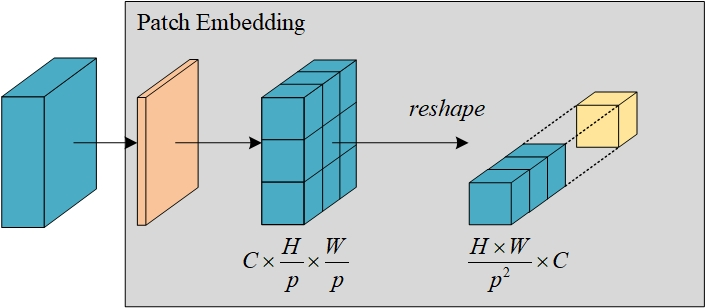
\includegraphics[width=0.5\columnwidth]{picture/LLIE/My Architecture/Patch Embedding}
		%\captionsetup{font=scriptsize}
		\caption{
			\label{fig: Patch Embedding} 
			嵌入块的一般性过程。
		}
	\end{figure}
	
	具体来说,对于原始的低光照图像 $P_1$,首先执行尺寸压缩操作,以适配预训练的视觉变换器(Vision Transformer, ViT)模型的权重。此操作将低光照图像(LLI)转换为一系列的Patch Embeddings,生成576个 D 维的特征向量,其中每个向量对应于一个$16 \times 16$的图像块(patch)。接下来,将$384 \times 384$的特征向量重排列为576个$16\times16$的图像块,每个图像块随后被展平(flatten)为256维的向量。考虑到图像的三通道特性,实际上每个通道被展平为256维,从而形成总计$256 \times 3$维的向量$\ell_1$。
	
	此过程的关键在于将二维图像数据转换为一维向量序列,这为后续的Transformer模型处理提供了适合的输入格式。通过这种方式,模型能够有效地处理图像数据,捕获重要的空间和颜色特征,从而为深度学习任务提供强大的数据基础。
	
	\begin{figure}[htb]
		% read manual to see what [ht] means and for other possible options
		\centering 
		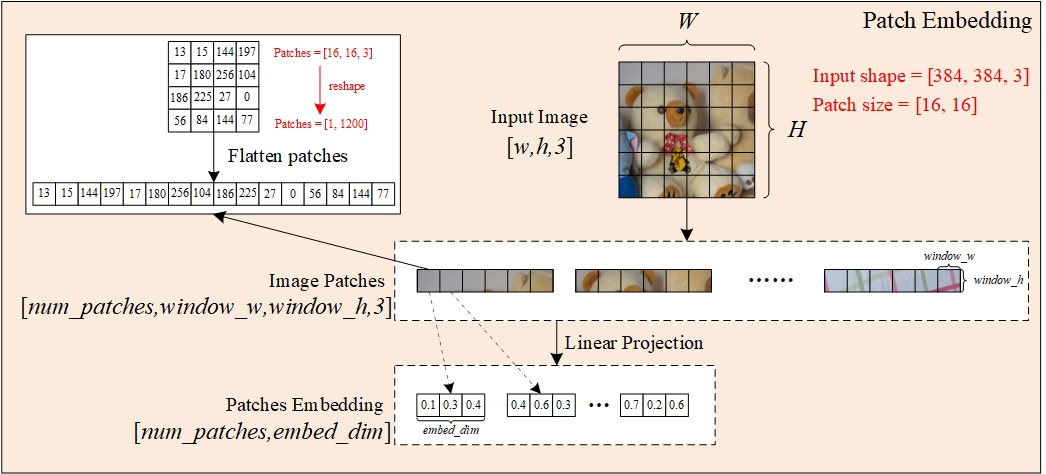
\includegraphics[width=0.8\columnwidth]{picture/LLIE/My Architecture/Patch Embedding(ViT)}
		%\captionsetup{font=scriptsize}
		\caption{
			\label{fig: Patch Embedding(ViT)} 
			Transformer 分支中嵌入块的过程。
		}
	\end{figure}
	
	为了进一步处理这些向量,我们采用一个线性投影(Linear Projection)操作,将$\ell_1$转换为D维的向量。这一转换过程不仅保留了原始图像块的关键信息,而且使其适配于深度学习模型的输入要求。如图\ref{fig: Patch Embedding(ViT)}所示,这一过程是将图像的空间特征转换为模型可以有效处理的形式的关键步骤。通过这种方式,模型能够更有效地处理和理解图像内容,从而在低光照图像增强任务中实现更优的性能。
	
	嵌入块的具体过程可以被描述为下列过程:
	
	\begin{itemize}
		\item[$\bullet$] 
		输入图像 $X \in \mathbb{R}^{H \times W \times C}$,其中 $H$,$W$和$C$ 分别代表图像的高度、宽度和通道数。
		\item[$\bullet$]
		图像被分割成 $N$ 个大小为 $P \times P$ 的块,每个块被展平并线性投影到 D 维空间,得到嵌入块 $E \in \mathbb{R}^{N \times D}$
	\end{itemize}
	
	图\ref{fig: First Architecture} 展示了在 Patch Embedding 过程之后,特征 $\mathcal{F}_1$ 经过必要的变换处理,以便与向量 $\ell_1$ 进行拼接操作。这一步骤是必要的,因为未经处理的特征 $\mathcal{F}_1$ 无法直接与向量 $\ell_1$ 进行有效的拼接。
	
	在本研究中,我们采用了 $20 \times 20$ 的 Patch 尺寸进行 Embedding。然而,选择此尺寸的适宜性依赖于输入图像的尺寸及其包含的细节的重要性。对于那些含有微小但关键特征的图像,较小的 Patch 尺寸可能更为适宜,因为它们能够更精确地捕捉这些细节。相反,较大的 Patch 尺寸可能更适合于捕获图像中的高层次抽象特征。因此,为了在细节捕捉和高层次特征表示之间找到最佳平衡点,我们的后续工作将包括对不同 Patch 尺寸的实验性探索,以确保模型能够有效地处理和理解图像中的关键信息。
	
	\paragraph{位置编码}
	
	在Transformer中,由于缺乏像卷积神经网络 (CNN) 那样的固有空间结构,需要一种方法来告知模型不同块之间的相对或绝对位置。位置编码就是为了解决这个问题而设计的。
	
	位置编码通常是通过将一个固定的或可学习的编码添加到每个块的 embedding 中来实现的。这个编码是根据块在原始图像中的位置计算得出的。一种常见的方法是使用正弦和余弦函数的组合来生成每个位置的编码。例如,对于位置 pos 和维度 i,编码可以被表示为式\ref{eq: positional encoding}
	
	\begin{equation}
		\begin{aligned}
			&\text{PE}(\text{pos}, \ 2i) = \sin \left(\frac{\text{pos}}{10000^{\frac{2i}{D}}}\right) \\
			&\text{PE}(\text{pos}, \ 2i + 1) = \cos \left(\frac{\text{pos}}{10000^{\frac{2i}{D}}}\right)
		\end{aligned}
		\label{eq: positional encoding}
	\end{equation}
	
	其中,D 是 embedding 的维度。计算出的 Positional Encoding 被加到每个 patch 的 embedding 上。位置编码为 $PE \in \mathbb{R}^{N \times D}$,Positional Encoding 被描述为 $E_{pos} = E + PE$。 这样,即使在多头自注意力机制中,模型也能够利用这些编码来理解和利用 patches 之间的相对位置信息。在ViT中,Positional Encoding对于模型理解图像内容至关重要。它允许模型捕捉到图像中的空间层次结构和对象之间的相对位置关系,这对于图像理解任务来说是非常重要的。
	
	我们采用 timm 库来创建预训练的ViT模型,并移除了原始的分类头,在 timm 库中创建的预训练 ViT 模型已经内置了Positional Encoding的过程。
	
	\paragraph{Transformer编码器}
	
	在视觉变换器 (ViT) 架构中,Transformer Encoder 是核心组件,负责处理图像的序列化表示。经过位置编码的 Patch Embeddings 被送入 Transformer 的编码器。如图\ref{fig: First Architecture} 所示,Transformer 编码器主要设计两个主要步骤,包括多头自注意力机制 (Multi-head Self-Attention) 和多层感知器 (Multi-Layer Perceptron)。这些组件共同工作,以捕获图像中的复杂特征和长距离依赖关系。
	
	其中,多头自注意力机制允许模型在处理每个图像块时同时考虑其他所有块的信息。通过这种方式,模型能够捕获图像中不同区域之间的复杂关系和依赖性。在多头自注意力中,注意力机制被分割成多个“头”,每个头学习图像的不同方面,从而提高了模型的表达能力。MLP 由多个线性层和非线性激活函数组成,它为模型引入了必要的非线性处理能力。这种非线性是处理复杂数据(如图像)时不可或缺的,因为它允许模型学习更加复杂和抽象的特征表示。
	
	对于每个 Transformer 层 $l$,输入 $X_l$ 经过以下过程:
	
	\begin{itemize}
		\item[1)] 
		多头自注意力 (MSA):
		\begin{equation}
			\begin{aligned}
				\text{MSA}(X_l) = [\text{head}_1, \text{head}_2, \ldots, \text{head}_k] W^{O}
			\end{aligned}
			\label{eq: MSA}
		\end{equation}
		其中每个头(head)是 $\text{head}_i = \text{Attention}\left(X_l W_i^Q, X_l W_i^K, X_l W_i^V \right)$。Attention 机制通常定义为
		\begin{equation}
			\begin{aligned}
				\text{Attention}(Q, K, V) = \text{softmax} \left(\frac{QK^T}{\sqrt{d_k}} \right) V
			\end{aligned}
			\label{eq: Attention}
		\end{equation}
		其中 $d_k$ 是 key 向量的维度。
		
		\item[2)]
		残差连接和层归一化:
		\begin{equation}
			\begin{aligned}
				X_l^\prime = \text{LayerNorm} \left(X_l + \text{MSA}(X_l)\right)
			\end{aligned}
			\label{eq: Residual Connection}
		\end{equation}
		
		\item[3)]
		多层感知机:
		MLP 包含两个全连接层和一个激活函数,即 $\text{MLP} (X_l^\prime) = \text{FC}\left(\text{GELU}\left(\text{FC}(X_l^\prime)\right)\right)$
		
		\item[4)]
		第二个残差连接和层归一化:
		\begin{equation}
			\begin{aligned}
				\displaystyle X_{l+1} = \text{LayerNorm} (X_l^\prime + \text{MLP}(X_l^\prime))
			\end{aligned}
			\label{eq: layernorm}
		\end{equation}
	\end{itemize}
	
	经过一层 Transformer编码器处理后,得到的输出 $X_L$ 可以用于下一步的处理。
	
	Transformer编码器通过多层自注意力和 MLP 的堆叠,有效地处理图像数据,捕获长距离依赖关系,并学习复杂的特征表示。这种架构使得模型能够处理高维度的图像数据,并提取有用的特征,为后续的图像处理任务提供强大的特征支持。
	
	\paragraph{特征耦合单元}
	
	在 PACUT 架构中,CNN 分支产生的特征映射与 Transformer 分支的 Patch Embedding 之间的有效融合是一个关键挑战。为了解决这一问题,我们引入了特征耦合单元(FCU),它通过交互式方法将局部特征与全局表示进行连续耦合,从而消除两者之间的不一致性。
	
	首先,我们认识到 CNN 分支和 Transformer 分支之间特征维度的不一致性。CNN 分支的特征图维度为$H \times W \times C$,其中$H$, $W$和$C$分别代表高度、宽度和通道数。而 Transformer 分支的嵌入块形状为$K \times D$,其中 $K$ 和 $D$ 分别表示图像块的数量和嵌入的维度。在用于分类的视觉变换器模型中,嵌入块的形状为$\left(K+1 \right) \times D$,其中额外的 1 代表类别嵌入(Class Token)。然而,在我们的 Transformer 分支中,我们去除了类别嵌入,以便更好地适应非分类任务。
	
	类别嵌入是一种特殊的嵌入,用于代表整个输入序列的全局信息。虽然这在图像分类任务中至关重要,但在图像增强等非分类任务中,其重要性相对较低。因此,去除类别嵌入不会显著影响特征图的恢复能力。
	
	为了实现 CNN 特征图和 Transformer Patch Embedding 之间的融合,我们首先通过$1 \times 1$卷积调整 CNN 特征图的通道维度,以匹配 Patch Embedding 的维度。接着,使用下采样模块(如图\ref{fig: Up-sampling and down-sampling} 所示)调整空间尺寸。完成这些步骤后,特征图与 Patch Embedding 进行融合(如图\ref{fig: First Architecture} 所示)。当特征从 Transformer 分支传输到 CNN 分支时,我们采用上采样(如图 \ref{fig: Up-sampling and down-sampling} 所示)来调整空间比例,并通过$ 1 \times 1$卷积调整通道尺寸,以便与 CNN 特征图对齐。此外,LayerNorm 和 BatchNorm 被用于特征的正则化。
	
	最后,考虑到特征映射和嵌入块之间存在的语义差异——前者源自局部卷积操作,后者则通过自注意力机制聚合——FCU 的应用至关重要,以填补这一语义鸿沟,确保两种特征的有效融合。
	
	\subsubsection{特征融合模块}
	
	在U型网络编码器结构中,浅层特征包含丰富的纹理信息和颜色信息,多层卷积得到的高层特征包含全局信息。对于弱光图像增强,需要尽可能的保留输出结果中的颜色信息。为此,PACUT 结构引入了图像通道来保留具由特定颜色特征的信息,从而更好的恢复暗区信息,防止亮区信息过度曝光。具体来说,在U型网络中设计了三个条约链接,将浅层特征发送到后头,以解决颜色信息丢失的问题。为了有效的融合视觉变换器和U型特征,提出一个如图\ref{fig: Fusion Block}所示的特征融合模块。其输入由两部分组成,即 PACUT 中CNN分支得到的特征 $\mathcal{F}_2$ 和Transformer分支中块展开(Patch Expanding)后得到的特征 $\mathcal{F}_3$。该模块包含两个步骤。
	
	\begin{figure}[h!]
		% read manual to see what [ht] means and for other possible options
		\centering 
		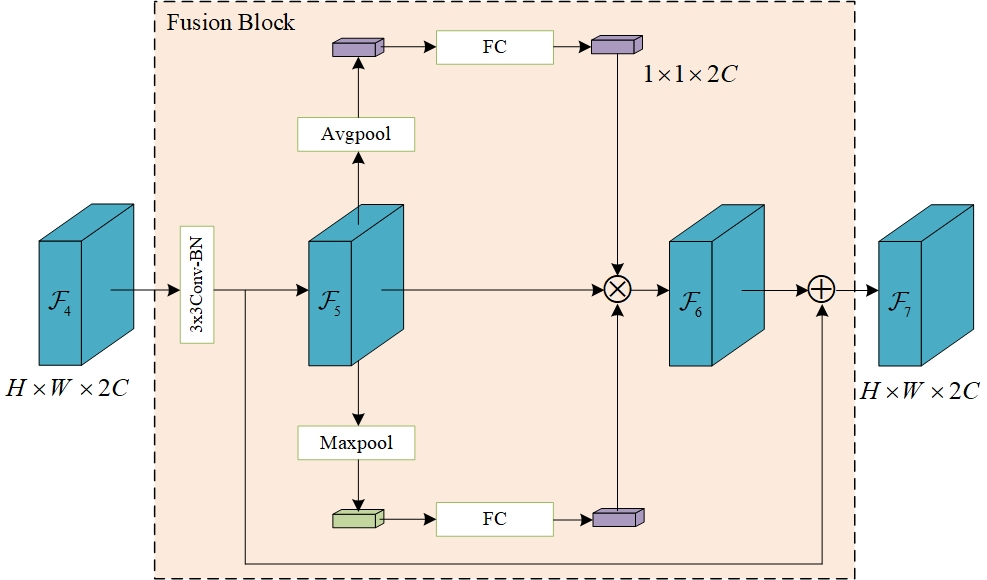
\includegraphics[width=0.7\columnwidth]{picture/LLIE/My Architecture/Fusion Block}
		%\captionsetup{font=scriptsize}
		\caption{
			\label{fig: Fusion Block} 
			融合模块的结构。
		}
	\end{figure}
	
	第一步,将两个尺寸为 $H \times W \times C$的特征图连接起来,形成一个尺寸为 $H \times W \times 2C$的特征图 $\mathcal{F}_4$。以该特征图为输入,通过 $3 \times 3$ 的卷积核,步长为1,进一步得到大小为 $H \times W \times 2C$ 的特征图 $\mathcal{F}_5$。这个过程可以有效的捕获颜色信息,表示为 
	\begin{equation}
		\begin{aligned}
			\mathcal{F}_5 = \delta \left( f^{3 \times 3} (\mathcal{F}_4)\right)
		\end{aligned}
		\label{eq: capture color information}
	\end{equation}
	
	在第二步中,通过为不同的通道分配适当的权重来重新校准特征映射 $\mathcal{F}_5$。为此,构建一个由两个加权支路和一个短连接组成的模块,如图\ref{fig: Fusion Block}所示。首先,通过全局平均池化将特征映射 $\mathcal{F}_5$ 压缩成 $1 \times 1 \times 2C$ 个向量;同时,特征映射 $\mathcal{F}_5$ 还需要进行全局最大池化,以尽可能的保留纹理细节。得到的 $1 \times 1 \times 2C$ 向量中的每一个元素表示通道信息。它们的公式为
	\begin{equation}
		\begin{aligned}
			\mathcal{Z}_{GAP} = \frac{1}{H \times W} \sum_{i}^{H} \sum_{j}^{W} {\mathcal{F}_5}_C (i,j)
		\end{aligned}
		\label{eq: avgpool}
	\end{equation}
	
	\begin{equation}
		\begin{aligned}
			\mathcal{Z}_{GMP} = \max \left( \mathcal{F}_5 \right)
		\end{aligned}
		\label{eq: maxpool}
	\end{equation}
	
	其中 $\mathcal{Z}_{GAP}$ 和 $\mathcal{Z}_{GMP}$ 分别为全局平均池化和全局最大池化得到的特征值,${\mathcal{F}_5}_C$ 为 $\mathcal{F}_5$ 的第 $C$ 个通道的特征。接下来,这两个压缩向量通过两个完全连接的层进行加权,以获得各自的权重向量。最后,通过特征向量乘以相应的权值,得到一个重新校准后,大小为 $H \times W \times 2C$ 的特征图 $\mathcal{F}_7$
	\begin{equation}
		\begin{aligned}
			\mathcal{F}_7 = \sigma \left( W_2 \delta (W_1 Z_{GAP}) \right) \cdot M \cdot \sigma \left( W_2 \delta (W_1 Z_{GMP})\right) +  \mathcal{F}_5
		\end{aligned}
		\label{eq: recalibrated feature map}
	\end{equation}
	其中 $W_1$ 和 $W_2$ 是两个完全连接层的权值。
	
	\subsubsection{损失函数}
	
	在本研究中,为了优化图像重建和内容生成的质量,我们提出了一个综合的联合损失函数,用于指导模型生成高质量的增强图像。该联合损失函数综合考虑了多个关键因素,以确保生成图像的质量和真实性。具体地,联合损失函数定义为:
	\begin{equation}
		\begin{aligned}
			\mathcal{L}_{all} = w_0 \mathcal{L}_{hub} + w_1 \mathcal{L}_{per} + w_2 \mathcal{L}_{\text{SSIM}}
		\end{aligned}
		\label{eq: loss function}
	\end{equation}
	其中,$\mathcal{L}_{hub}$ 代表休伯(Huber)损失\cite{huber1992robust},$\mathcal{L}_{per}$代表感知损失\cite{johnson2016perceptual},而$\mathcal{L}_{\text{SSIM}}$代表结构相似性(SSIM)损失\cite{wang2004image}。这些损失函数的组合旨在平衡图像的像素级精度和感知质量。
	
	Huber 损失($\mathcal{L}_{hub}$)是一种结合了均方误差和绝对误差的损失函数,用于减少对异常值的敏感性,从而提高模型的鲁棒性。感知损失($\mathcal{L}_{per}$)则关注于图像的高级特征和内容,通过比较深层网络中的特征表示来评估图像之间的感知差异。结构相似性指数(SSIM)损失($\mathcal{L}_{\text{SSIM}}$)则用于评估图像的结构、亮度和对比度等方面的相似性,以确保生成图像在视觉上与原始图像保持一致性。
	
	权重$w_0$, $w_1$和$w_2$分别对应于这三种损失的相对重要性,通过实验调整以达到最佳的图像增强效果。通过这种方式,联合损失函数能够有效地平衡像素级精度和感知质量,从而生成在视觉上更加令人满意的增强图像。
	
	我们设$w_0 = 1$, $w_1 = 0.006$和$w_2 = 0.01$。
	
	通过最小化PACUT的输出与正常照明图像之间的误差,利用休伯损失指导PACUT生成结构完整的增强图像。令$I_{GT}$为真实图像,$I_{EI}$为增强图像。休伯损失可以表示为式\ref{eq: huber loss}
	\begin{equation}
		\mathcal{L}_{hub}(\delta)= \frac{1}{N}\sum_{i=1}^{N}
		\left\{
		\begin{aligned}
			&\displaystyle{\frac{1}{2}{\left\|I_{\text{GT}} - I_{\text{EI}} \right\|}_2^{2}, \left\| I_{GT} -I_{EI} \right\| < \delta }, \\
			&\delta\left({\left\|I_{\text{GT}} - I_{\text{EI}} \right\|}_1 - \frac{1}{2}\delta \right), \left\| I_{\text{GT}} -I_{\text{EI}} \right\| \geq \delta.
		\end{aligned}
		\label{eq: huber loss}
		\right.
	\end{equation}
	$\mathcal{L}_2$-loss但容易受离群点的影响,$\mathcal{L}_1$-loss对离群点更加健壮但是收敛慢,Huber Loss 则是一种将 MSE 与 MAE 结合起来,取两者优点的损失函数,也被称作Smooth Mean Absolute Error Loss。其原理很简单,就是在误差接近0时使用$\mathcal{L}_2$-loss,误差较大时使用$\mathcal{L}_1$-loss
	
	然而,休伯损失容易同时平滑增强图像的噪点和细节。为了保留图像的纹理信息,提高图像内容质量,我们引入感知损失,用于比较图像之间的高层次差异,感知损失可以表示为式\ref{eq: perceptual loss}。
	\begin{equation}
		\begin{aligned}
			\mathcal{L}_{feat}^{\phi,j} (I_{GT},I_{EI}) = \frac{1}{C_{j}H_{j}W_{j}}{\left\| \phi_{j}(I_{GT})-\phi_{j}(I_{EI})\right\|}_{2}^2
		\end{aligned}
		\label{eq: perceptual loss}
	\end{equation}
	
	其中$I_{GT}$为输出图像,$I_{EI}$为目标图像,$\phi$为损失网络。$\phi_{j}(x)$为处理图像$x$时损失网络$\phi$的第$j$层的激活情况,如果$j$是一个卷积层,那么$\phi_{j}(x)$将是形状$C_{j} \times H_{j} \times W_{j}$的特征映射,特征重建损失是特征表示之间的欧式距离。
	
	此外,为了使得恢复图像的亮度、对比度和结构与真实图像更加接近和同时细化恢复图像的细节,我们引入了结构相似性损失,结构相似性损失可以表示为式
	
	每个像素$p$的\text{SSIM}被定义为式\ref{eq: revised_SSIM loss}
	\begin{equation}
		\begin{aligned}
			\text{SSIM}(p) &= \frac{2\mu_{x}\mu_{y}+C_{1}}{\mu_{x}^2+\mu_{y}^2+C_{1}} \cdot \frac{2\sigma_{xy}+C_{2}}{\sigma_{x}^2+\sigma_{y}^{2}+C_{2}} \\
			&= l(p)\cdot cs(p)
		\end{aligned}
		\label{eq: SSIM}
	\end{equation}
	
	其中省略了均值和标准偏差对像素$p$的依赖性,均值和标准差是用标准偏差为$\sigma_G,G_{\sigma_G}$
	\begin{equation}
		\begin{aligned}
			&\varepsilon(p)=1-\text{SSIM}(p): \\  &\mathcal{L}^{\text{SSIM}}(P)=\frac{1}{N}\sum_{p \in P}1-\text{SSIM}(p).
		\end{aligned}
		\label{eq: SSIM loss}
	\end{equation}
	
	式\ref{eq: SSIM}表明$\text{SSIM}(p)$需要关注像素$p$的邻域,这个领域的大小取决于$G_{\sigma_G}$,网络的卷积性质允许我们将SSIM损失写为
	\begin{equation}
		\begin{aligned}
			\mathcal{L}^{\text{SSIM}}(P)=1-\text{SSIM}(\tilde{p}).
		\end{aligned}
		\label{eq: revised_SSIM loss}
	\end{equation}
	
	其中$\tilde{p}$是$P$的中心像素。
	
	\subsection{边缘检测网络}
	
	\subsubsection{现有方法的局限性}
	
	边缘检测是视觉任务中非常基础的任务,现有的基于 CNN 的边缘检测方法有两个明显的问题。
	
	\begin{itemize}
		\item [(1)] 首先,当前大多数方法主要依赖于 CNN 的最终层(通常是最后一层卷积层)的输出,而忽视了网络中间层的潜在价值。这种做法可能导致信息的丢失,特别是那些在中间层中更为显著的特征信息。
		
		\item [(2)] 虽然研究者们普遍关注于探索更深层次的 CNN 结构,但在边缘检测这一特定任务中,这种方法面临着数据稀缺性和梯度消失问题的双重挑战。由于边缘检测任务通常涉及的数据量相对较少,加之深层网络易于出现梯度消失,这些因素共同制约了深层 CNN 在边缘检测领域的应用效果。
	\end{itemize}

	Liu\cite{liu2017richer}发现不同卷积层获得的结果随着深度增加而更加粗糙(如图\ref{fig: Motivation of RCF}所示),其提出 RCF(Richer convolutional features) 方法充分利用所有 CNN 层的结果。相比之下,HED (Holistically-nested edge detection) \cite{xie2015holistically}方法仅采用了 VGG16 架构中每个阶段的最后一层卷积输出,而 RCF (Richer Convolutional Features) 方法则利用了每个层级的卷积结果。这一策略使得 RCF 在捕获丰富的边缘信息方面展现了更为显著的能力。

	\begin{figure}[htb] 
		\centering 		
		\begin{subfigure}{0.2\textwidth}
			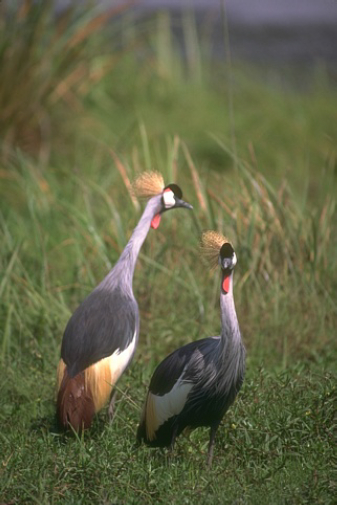
\includegraphics[width=\linewidth]{picture/LLIE/RCF/origin image}
			\captionsetup{font=scriptsize}
			\caption{origin image}
			\label{fig: origin image}
		\end{subfigure}
		\begin{subfigure}{0.2\textwidth}
			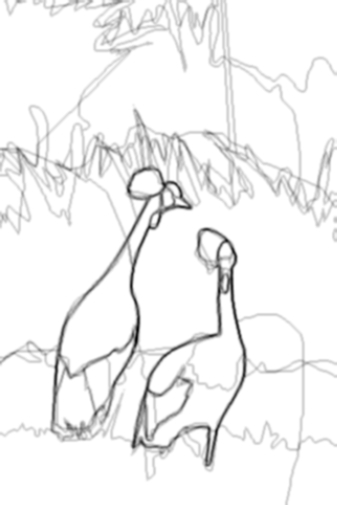
\includegraphics[width=\linewidth]{picture/LLIE/RCF/GT}
			\captionsetup{font=scriptsize}
			\caption{GT}
			\label{fig: RCF_GT}
		\end{subfigure}
		\begin{subfigure}{0.2\textwidth}
			\includegraphics[width=\linewidth]{picture/LLIE/RCF/conv3_1}
			\captionsetup{font=scriptsize}
			\caption{conv3\_1}
			\label{fig: conv3_1}	
		\end{subfigure}
		\begin{subfigure}{0.2\textwidth}
			\includegraphics[width=\linewidth]{picture/LLIE/RCF/conv3_2}
			\captionsetup{font=scriptsize}
			\caption{conv3\_2}
			\label{fig: conv3_2}	
		\end{subfigure}\\
		\begin{subfigure}{0.2\textwidth}
			\includegraphics[width=\linewidth]{picture/LLIE/RCF/conv3_3}
			\captionsetup{font=scriptsize}
			\caption{conv3\_3}
			\label{fig: conv3_3}
		\end{subfigure}
		\begin{subfigure}{0.2\textwidth}
			\includegraphics[width=\linewidth]{picture/LLIE/RCF/conv4_1}
			\captionsetup{font=scriptsize}
			\caption{conv4\_1}
			\label{fig: conv4_1}
		\end{subfigure}
		\begin{subfigure}{0.2\textwidth}
			\includegraphics[width=\linewidth]{picture/LLIE/RCF/conv4_2}
			\captionsetup{font=scriptsize}
			\caption{conv4\_2}
			\label{fig: conv4_2}	
		\end{subfigure}
		\begin{subfigure}{0.2\textwidth}
			\includegraphics[width=\linewidth]{picture/LLIE/RCF/conv4_3}
			\captionsetup{font=scriptsize}
			\caption{conv4\_3}
			\label{fig: conv4_3}	
		\end{subfigure}
		%\captionsetup{font=scriptsize}
		\caption{
			\label{fig: Motivation of RCF}
			建立了一个基于 VGG16\cite{simonyan2014very} 的简单网络来产生侧输出(c-h)。我们可以看到,卷积特征逐渐变得更粗,而中间层(c、d、f、g)包含了在其他层中没有出现的基本细节。
		}
	\end{figure}
	\FloatBarrier

	此外,获取边缘图的方法也各不相同,在 LLIE 任务中,常见方法采用边缘检测网络来生成边缘图,然后使用 Canny 或 Sobel 算子\cite{maini2009study}从 GT 中获取边缘图用做对照组。目前在 LLIE 领域中获取边缘图分化成了两个不同的方向,一种是通过初步恢复图像获取边缘图(见图\ref{fig: EEMEFN}),另一种是直接通过弱光图像以获取边缘图(见图\ref{fig: EdgeNet}和图\ref{fig: SMG-LLIE Architecture})。LLIE 任务中边缘检测的主要有下列方法:
	
	在LLIE(低光照图像增强)任务中,边缘检测技术的应用可概括为以下几种主要方法:
	
	\begin{itemize}
		\item [(1)] 利用手工设计的各类滤波器生成边缘图像。
		
		\item [(2)] 采用基于人类设计特征的数据驱动模型(如使用随机决策森林)来预测边缘。
		
		\item [(3)] 通过深度学习技术,从原始数据中学习复杂的特征表示,实现端到端的边缘检测模型(例如RCF边缘检测模型\cite{liu2017richer})。
	\end{itemize}

	经过广泛的文献综述,我们发现在LLIE领域内,边缘图像的获取主要分为两个不同的路径:一是从初步恢复的图像中提取边缘图(如图\ref{fig: EEMEFN}所示),二是直接从低光照图像中提取边缘图(如图\ref{fig: EdgeNet}和图\ref{fig: SMG-LLIE Architecture}所示)。传统方法如 Canny 和 Sobel 算子\cite{maini2009study}在直接从低光照图像中提取边缘时面临较大挑战,如图\ref{fig: LLI_canny}所示。然而,基于深度学习的方法能从低光照图像中提取出更为详细的边缘图像,虽然与真实边缘仍有差异。我们的研究目标是缩减这一差距,以提高基于结构建模指导的模型的准确性。本研究尝试使用不同曝光度的图片,获取它们的 HOG 和 LBP 图像,并采用多曝光图像融合架构,从而获得更接近真实边缘结构的边缘图像,其结构示意见图\ref{fig: Edge Detection Network}。

	\begin{figure}[htb]
		\centering
		\begin{subfigure}{0.19\textwidth}
			\includegraphics[width=\linewidth]{picture/LLIE/My Architecture/Edge Detection/low00044}
			\captionsetup{font=scriptsize}
			\caption{LLI}
			\label{fig: LLI}
		\end{subfigure}
		\begin{subfigure}{0.19\textwidth}
			\includegraphics[width=\linewidth]{picture/LLIE/My Architecture/Edge Detection/low00044_canny}				
			\captionsetup{font=scriptsize}
			\caption{LLI Canny}
			\label{fig: LLI_canny}	
		\end{subfigure}
		\begin{subfigure}{0.19\textwidth}
			\includegraphics[width=\linewidth]{picture/LLIE/My Architecture/Edge Detection/low00044_rcf}
			\captionsetup{font=scriptsize}
			\caption{LLI RCF}
			\label{fig: LLI_rcf}
		\end{subfigure}
		\begin{subfigure}{0.19\textwidth}
			\includegraphics[width=\linewidth]{picture/LLIE/My Architecture/Edge Detection/low00044_hog}
			\captionsetup{font=scriptsize}
			\caption{LLI HOG}
			\label{fig: LLI_hog}
		\end{subfigure}
		\begin{subfigure}{0.19\textwidth}
			\includegraphics[width=\linewidth]{picture/LLIE/My Architecture/Edge Detection/low00044_lbp}
			\captionsetup{font=scriptsize}
			\caption{LLI LBP}
			\label{fig: LLI_lbp}
		\end{subfigure}\\
		\begin{subfigure}{0.19\textwidth}
			\includegraphics[width=\linewidth]{picture/LLIE/My Architecture/Edge Detection/normal00044}
			\captionsetup{font=scriptsize}
			\caption{GT}
			\label{fig: GI}
		\end{subfigure}
		\begin{subfigure}{0.19\textwidth}
			\includegraphics[width=\linewidth]{picture/LLIE/My Architecture/Edge Detection/normal00044_canny}
			\captionsetup{font=scriptsize}
			\caption{GT Canny}
			\label{fig: GT_canny}
		\end{subfigure}
		\begin{subfigure}{0.19\textwidth}
			\includegraphics[width=\linewidth]{picture/LLIE/My Architecture/Edge Detection/normal00044_rcf}
			\captionsetup{font=scriptsize}
			\caption{GT RCF}
			\label{fig: GT_rcf}
		\end{subfigure}
		\begin{subfigure}{0.19\textwidth}
			\includegraphics[width=\linewidth]{picture/LLIE/My Architecture/Edge Detection/normal00044_hog}
			\captionsetup{font=scriptsize}
			\caption{GT HOG}
			\label{fig: GT_hog}	
		\end{subfigure}
		\begin{subfigure}{0.19\textwidth}
			\includegraphics[width=\linewidth]{picture/LLIE/My Architecture/Edge Detection/normal00044_lbp}
			\captionsetup{font=scriptsize}
			\caption{GT LBP}
			\label{fig: GT_lbp}	
		\end{subfigure}
		\caption{
			\label{fig: LLI Structure Information}
			基于 LOL-v2 弱光数据集的边缘信息。
		}
	\end{figure}
	\FloatBarrier

	%现在的方法大多只使用 CNN 的最后一层 conv 的结果,忽略了中间层的结果。
		
	%更多的方法集中在探究更深的 CNN,但边缘检测是数据比较少,而且容易发生梯度消失的现象。
	
	\begin{figure}[htb]
		% read manual to see what [ht] means and for other possible options
		\centering 
		\includegraphics[width=\columnwidth]{picture/LLIE/My Architecture/Edge Detection Network}
		%\captionsetup{font=scriptsize}
		\caption{
			\label{fig: Edge Detection Network} 
			边缘检测网络。
		}
	\end{figure}
	\FloatBarrier
	
	\begin{figure}[htb]
		% read manual to see what [ht] means and for other possible options
		\centering 
		\includegraphics[width=\columnwidth]{picture/LLIE/My Architecture/Total architecture}
		\caption{
			\label{fig: Total Architecture} 
			我们提出的网络结构。
		}
	\end{figure}
	\FloatBarrier
	
	\part*{具体工作内容}
	
	\section{已完成工作}
	
	\subsection{初步恢复图像的生成模型实验结果}
	
	我们针对初步恢复图像的生成模型进行了实验验证,以验证所提出方法的有效性。首先,介绍了实验的具体实施细节,包括网络的实现、所采用的数据集以及评估指标的选择。接着,通过与当前领先技术的比较分析,展示了我们网络在低光图像增强任务中的性能优势。最后,为了深入理解各个网络组件的贡献,我们执行了一系列消融研究,探讨了这些组件在低光图像增强任务中的作用和重要性。
	
	具体来说,实验设置部分详细描述了网络的配置、训练过程中的参数设置、以及用于训练和测试的数据集特性。此外,本研究采用的评估指标被精心选取,以全面反映图像增强的效果,包括定量指标和定性分析。
	
	在性能比较部分,我们的方法与当前最先进的低光图像增强技术进行了对比。这一比较不仅基于传统的性能指标,如图像质量评分,还包括了对增强效果的视觉评估,以展示我们方法的综合优势。
	
	最后,消融实验部分旨在揭示网络各个组成部分的相对重要性和功能。通过系统地移除或修改网络的特定部分,我们能够评估每个组件对最终增强效果的贡献,从而深入理解整个网络的工作机制。这些实验结果为我们的网络设计提供了进一步的洞察和验证。
	
	\subsubsection{实验设置}
	
	在实验实施方面,模型是基于 Pytorch 框架进行实现的。为了确定 Transformer 分支的最优输入图像尺寸,我们分别设置了 384x384 和 224x224 两种分辨率,并通过一系列实验来确定最佳的预训练图像尺寸。在模型训练过程中,我们采用了 Adam 优化器,其权重衰减系数设定为 0.00001,以减少过拟合的风险。此外,模型中所有层的学习率统一设置为 0.0001,以确保训练过程的稳定性和收敛性。
	
	基于硬件资源和内存限制的考虑,我们将训练的批处理大小设定为 8。同时,为了充分训练模型并确保其泛化能力,我们将训练的 epoch 数设置为200。所有的实验均在配备 NVIDIA GeForce RTX 4090 显卡的计算平台上进行,以确保训练和测试过程的高效性和可靠性。
	
	\subsubsection{数据集和评价指标}
	
	为了全面评估我们所提出网络的性能,我们对两个公共数据集(LOL\cite{wei2018deep}和SCIE\cite{cai2018learning})进行了实验评估。在评估过程中,我们使用了峰值信噪比(PSNR)\cite{wang2004image}、结构相似度(SSIM)\cite{wang2004image}以及自然图像质量评估器(NIQE)\cite{mittal2012making}等度量指标,以全面衡量图像增强结果的质量。这些评价指标旨在提供对重建图像质量的客观评估,从而深入了解我们提出的网络在低光照环境下的性能表现。
	
	\subsubsection{对比试验}
	
	我们将所提算法的结果与多个公开可获得的代码进行比较,包括HE\cite{pisano1998contrast}、LightenNet\cite{li2018lightennet}、LLNet\cite{lore2017llnet}、Retinex-Net\cite{wei2018deep}、MBLLEN\cite{lv2018mbllen}、EnlightenGAN\cite{jiang2021enlightengan}、Zero-DCE\cite{guo2020zero}以及KinD\cite{zhang2019kindling}。
	
	\begin{table}[!htbp]
		\centering
		\tiny
		\resizebox{\textwidth}{!}{ %按照宽度调整调整表格大小
				\begin{tabular}{>{\centering\arraybackslash}m{2.5cm}|c|c|c|c|c|c}
						
						\hline %添加表格头部粗线
						
						\multirowcell{2}{\textbf{Method}} & \multicolumn{3}{c|}{\makecell{\textbf{LOL}\cite{wei2018deep}}} & \multicolumn{3}{c}{\makecell{\textbf{SCIE}\cite{cai2018learning}}} \\
						
						\cline{2-7}
						
						
						      & \textbf{PSNR↑} & \textbf{SSIM↑} & \textbf{NIQE↓} & \textbf{PSNR↑}  & \textbf{SSIM↑} & \textbf{NIQE↓} \\
						
						\hline
						
						input & 7.773 & 0.181 & 0.560 & 17.824 & 0.779 & 0.148  \\
						
						\hline	
						
						HE\cite{pisano1998contrast}             & 15.467 & 0.504 & 9.531 & 15.342 & 0.741 & 9.232 \\
						LightenNet\cite{li2018lightennet}       & 10.301 & 0.361 & 7.422 & 13.579 & 0.744 & 8.166 \\
						LLNet\cite{lore2017llnet}               & \textcolor{blue}{17.953} & 0.704 & \textcolor{red}{3.974} & 12.177 & 0.645 & 4.292 \\
						Retinex-Net\cite{wei2018deep}           & 16.774 & 0.462 & 5.474 & 12.310 & 0.671 & 7.239 \\ 
						KinD\cite{zhang2019kindling} 	          & 16.648 & \textcolor{blue}{0.779} & 6.175 & 21.103 & \textcolor{red}{0.838} & 4.195 \\
						MBLLEN\cite{lv2018mbllen}               & 17.902 & 0.715 & \textcolor{blue}{4.247} & 13.638 & 0.632 & \textcolor{blue}{2.108} \\
						EnlightenGAN\cite{jiang2021enlightengan}& 17.483 & 0.658 & 4.889 & 18.726 & 0.822 & 5.216 \\
						Zero-DCE\cite{guo2020zero}              & 17.622 & 0.556 & 7.972 & \textcolor{red}{22.682} & 0.810 & \textcolor{red}{1.158} \\
						\textbf{Ours}                             & \textcolor{red}{22.780} & \textcolor{red}{0.823} & 4.473 & \textcolor{blue}{21.543} & \textcolor{blue}{0.835} & 3.412 \\
						\hline
						
					\end{tabular}
			}
		%\captionsetup{font=scriptsize} %设置标题字体与表格字体一致
		\caption{
				\label{tab: Quantitative Comparisons on LOL-test and SCI testing datasets}
				LOL和SCIE数据集在各方法下的对比值,其中红色表示最优,蓝色表示次优,$↑$表示越高越好,$↓$表示越低越好。
				} 
	\end{table}
	
	本研究通过对 LOL 数据集的全面评估展示了所提出模型与其他方法的整体性能,具体结果见表\ref{tab: Quantitative Comparisons on LOL-test and SCI testing datasets}。在LOL测试数据集上,我们的模型展现出卓越的性能,其 PSNR 和 SSIM 达到最佳水平。在 SCIE 测试数据集上,尽管 PSNR 和 SSIM 相对较低,但仍表现出令人满意的效果,验证了模型的有效性。
	
	\begin{figure}[htb] 
		\centering 
		\begin{subfigure}{0.19\textwidth}
			\includegraphics[width=\linewidth]{picture/LLIE/Efficent/Input}
			\captionsetup{font=scriptsize}
			\caption{Input}
			\label{fig: LLI Input}
		\end{subfigure}
		\begin{subfigure}{0.19\textwidth}
			\includegraphics[width=\linewidth]{picture/LLIE/Efficent/LightenNet}
			\captionsetup{font=scriptsize}
			\caption{LightenNet}
			\label{fig: LightenNet}
		\end{subfigure}
		\begin{subfigure}{0.19\textwidth}
			\includegraphics[width=\linewidth]{picture/LLIE/Efficent/LLNet}				
			\captionsetup{font=scriptsize}
			\caption{LLNet}
			\label{fig: LLI LLNet}	
		\end{subfigure}
		\begin{subfigure}{0.19\textwidth}
			\includegraphics[width=\linewidth]{picture/LLIE/Efficent/RetinexNet}
			\captionsetup{font=scriptsize}
			\caption{RetinexNet}
			\label{fig: LLI RetinexNet}	
		\end{subfigure}
		\begin{subfigure}{0.19\textwidth}
			\includegraphics[width=\linewidth]{picture/LLIE/Efficent/KinD}
			\captionsetup{font=scriptsize}
			\caption{KinD}
			\label{fig: KinD}	
		\end{subfigure}\\
		\begin{subfigure}{0.19\textwidth}
			\includegraphics[width=\linewidth]{picture/LLIE/Efficent/MBLLEN}
			\captionsetup{font=scriptsize}
			\caption{MBLLEN}
			\label{fig: MBLLEN}	
		\end{subfigure}
		\begin{subfigure}{0.19\textwidth}
			\includegraphics[width=\linewidth]{picture/LLIE/Efficent/EnlightenGAN}
			\captionsetup{font=scriptsize}
			\caption{EnlightenGAN}
			\label{fig: LLI EnlightenGAN}	
		\end{subfigure}
		\begin{subfigure}{0.19\textwidth}
			\includegraphics[width=\linewidth]{picture/LLIE/Efficent/Zero-DCE}
			\captionsetup{font=scriptsize}
			\caption{Zero-DCE}
			\label{fig: Zero-DCE}	
		\end{subfigure}
		\begin{subfigure}{0.19\textwidth}
			\includegraphics[width=\linewidth]{picture/LLIE/Efficent/Ours}
			\captionsetup{font=scriptsize}
			\caption{Ours}
			\label{fig: Ours}	
		\end{subfigure}
		\begin{subfigure}{0.19\textwidth}
			\includegraphics[width=\linewidth]{picture/LLIE/Efficent/GT}
			\captionsetup{font=scriptsize}
			\caption{GT}
			\label{fig: GT}	
		\end{subfigure}
		%\captionsetup{font=scriptsize}
		\caption{
			\label{fig: LOL}
			不同方法在LOL测试数据集上的视觉表现。
		}
	\end{figure}
	
	图\ref{fig: LOL}展示了各种方法在LOL测试数据集上的图像增强效果,其中 GT 表示真实图片。与Zero-DCE、LLNet和MBLLEN相比,RetinexNet呈现出颜色饱和度更强的增强效果,而Zero-DCE、LLNet和MBLLEN的结果在视觉上偏暗。EnlightenGAN在增强的图像中显示出明显的灰色伪影,表明其对噪声较为敏感。尽管我们的方法相对真实值而言稍显偏亮,但在LOL数据集上表现出优于对比方法的效果。
	
	\subsection{消融实验}
	
	我们采用PSNR、SSIM和NIQE指标,对SCConv模块、Transformer分支以及基于不同尺寸的预训练视觉变换器模型的有效性进行评估。我们设定去除SCConv模块的CNN分支作为基线网络。如表\ref{tab: Ablation Study}所示,引入Transformer分支并增加输入到Transformer分支的特征图尺寸,相较于基线,模型性能得到了显著改善。
	
	\begin{table}[!htbp]
		\centering
		\tiny
		\resizebox{\textwidth}{!}{ %按照宽度调整调整表格大小
			\begin{tabular}{c|c|c|c|c|c|c}
						
					\hline
						
					\textbf{基线模型} & \textbf{SCConv} & \textbf{Transformer分支} & \textbf{Transformer预训练权重尺寸}  & \textbf{PSNR↑} & \textbf{SSIM↑} & \textbf{NIQE↓} \\
			
					\hline
					
					\checkmark &            &            &                  & 18.222 & 0.642 & 7.213 \\
					\checkmark & \checkmark &            &                  & 18.231 & 0.523 & 5.231 \\
					\checkmark & \checkmark & \checkmark & $224 \times 224$ & 21.643 & 0.815 & 4.552 \\
					\checkmark & \checkmark & \checkmark & $384 \times 384$ & \textbf{22.780} & \textbf{0.823} & \textbf{4.473} \\
		
					\hline			
			\end{tabular}
		}
		%\captionsetup{font=scriptsize} %设置标题字体与表格字体一致
		\caption{
			\label{tab: Ablation Study}
			Transformer分支和Transformer预训练权重尺寸和SCConv对模型的影响。
		} 
	\end{table}
	
	\section{下一步工作}
	
	接下来主要工作主要从以下方面开展:
	
	通过完善文献调研工作进一步阐述弱光图像恢复的重要性及其在当前研究领域的挑战性,包括强调边缘信息在图像处理中的关键作用。此外,进一步明确提出研究的主要目标。综述现有文献,包括边缘检测技术、低光图像恢复方法以及Transformer网络的应用。分析现有方法的局限性,并探讨潜在的改进方向。
	
	总结下来分为以下三个方面:
	\begin{itemize}
		\item[(1)] \textbf{边缘检测网络评价指标的研究:}确立用于评估边缘检测网络性能的关键指标,如精度、召回率和F1分数等。此外,设计实验以量化评估不同边缘检测方法在低光条件下的表现。
		
		\item[(2)] \textbf{实验设计与验证:}使用现有边缘检测模型(例如RCF)进行初步实验,评估其在弱光图像恢复中的效果。对比分析现有技术与改进方法的性能差异。
		
		\item[(3)] \textbf{改进方案的探索与实现:}尝试结合 RCF 方法和 Transformer 模型,设计新的边缘检测与图像恢复模型,并在标准数据集上测试新模型,并与传统方法进行性能比较。
	\end{itemize}
	
	\renewcommand{\refname}{参考文献}
	
	
	%	\begin{thebibliography}{00}
		
		%		\bibitem{b1}\label{cite:b1}
		%		W. Wang, C. Wei, W. Yang and J. Liu, "GLADNet: Low-Light Enhancement Network with Global Awareness," 2018 13th IEEE International Conference on Automatic Face \& Gesture Recognition (FG 2018), Xi'an, China, 2018, pp. 751-755, DOI: 10.1109/FG.2018.00118.
		
		%		\bibitem{b2}\label{cite:b2}
		%		A.\ Mahajan, K.\ Somaraj and M. Sameer, "Adopting Artificial Intelligence Powered ConvNet To Detect Epileptic Seizures," 2020 IEEE-EMBS Conference on Biomedical Engineering and Sciences (IECBES), Langkawi Island, Malaysia, 2021, pp. 427-432, DOI: 10.1109/IECBES48179.2021.9398832.
		
		%		\bibitem{Cyr}
		%		N.\ Cyr, M.\ T$\hat{e}$tu, and M.\ Breton,
		% "All-optical microwave frequency standard: a proposal,"
		%		IEEE Trans.\ Instrum.\ Meas.\ \textbf{42}, 640 (1993).
		
		
		
		%	\end{thebibliography}
	
	\bibliographystyle{unsrt}
	\bibliography{reference}
	
	
\end{document}
